% options:
% thesis=B bachelor's thesis
% thesis=M master's thesis
% czech thesis in Czech language
% english thesis in English language
% hidelinks remove colour boxes around hyperlinks

% TODO:
% * Zvolit správné Prohlášení
% * Opravit footnotes v tabulkách

% arara: xelatex: { shell: yes }
% arara: makeglossaries	
% arara: biber
% arara: xelatex: { shell: yes }
% arara: xelatex: { shell: yes }
% arara: xelatex: { shell: yes }
\documentclass[thesis=M,czech,hidelinks]{../template/FITthesisXE}

\usepackage{ booktabs }		% for prettier tables
\usepackage{ dirtree } 		% directory tree visualisation
\usepackage{ graphicx }		% graphics files inclusion
\usepackage{ longtable } 	% tables which Pandoc use
\usepackage{ lscape }		% to be able to rotate stuff
\usepackage{ makecell }		% for newlines in table cells
\usepackage{ mdframed }		% hack for bg colors in minted
\usepackage{ metalogo }		% for \XeLaTeX
\usepackage{ multicol }		% for multiple columns
\usepackage{ multirow }		% for multiple rows
\usepackage{ rotating }		% for rotating pictures
\usepackage{ xcolor } 		% for custom colors
\usepackage{ xevlna }		% for non-breakable whitespaces

\bibliography{sources.bib}

% make list of acronyms
\makeglossaries
\newacronym{API}{API}{Application Programming Interface}
\newacronym{ARES}{ARES}{Administrativní registr ekonomických subjektů}
\newacronym{BSD}{BSD}{Berkeley Software Distribution}
\newacronym{CDN}{CDN}{Content Delivery Network}
\newacronym{CI}{CI}{Continuous Integration}
\newacronym{CLI}{CLI}{Command Line Interface}
\newacronym{CORS}{CORS}{Cross-origin resource sharing}
\newacronym{CSS}{CSS}{Cascading Style Sheets}
\newacronym{DI}{DI}{Dependency Injection}
\newacronym{DPH}{DPH}{Daň z přidané hodnoty}
\newacronym{E2E}{E2E}{End-to-end}
\newacronym{EAN}{EAN}{European Article Number}
\newacronym{ES}{ES}{ECMAScript}
\newacronym{FIT}{FIT}{Fakulta informačních technologií}
\newacronym{GUI}{GUI}{Graphical User Interface}
\newacronym{HTML}{HTML}{Hypertext Markup Language}
\newacronym{IBAN}{IBAN}{International Bank Account Number}
\newacronym{IDE}{IDE}{Integrated Development Environment}
\newacronym{IČO}{IČO}{Identifikační číslo osoby}
\newacronym{JS}{JS}{Javascript}
\newacronym{MIT}{MIT}{Massachusetts Institute of Technology}
\newacronym{MI}{MI}{Magisterská Informatika}
\newacronym{NPM}{NPM}{Node Package Manager}
\newacronym{NUR}{NUR}{Návrh uživatelského rozhraní}
\newacronym{OOP}{OOP}{Objektově orientované programování}
\newacronym{OS}{OS}{Operační Systém}
\newacronym{PDF}{PDF}{Portable Document Format}
\newacronym{PHP}{PHP}{PHP: Hypertext Preprocessor}
\newacronym{SASS}{SASS}{Syntactically Awesome Style Sheets}
\newacronym{SPA}{SPA}{Single Page Application}
\newacronym{SVN}{SVN}{Subversion}
\newacronym{TDD}{TDD}{Test-driven development}
\newacronym{UI}{UI}{User Interface}
\newacronym{URL}{URL}{Uniform Resource Locator}
\newglossaryentry{gBackend}{
	name=Backend,
	description={
		Část aplikace, která se stará o ukládání dat, jejich zpracování a bussiness logiku. Většinou není přímo přístupná koncovému uživateli, ten k ní přistupuje přes frontend.
	}
}
\newglossaryentry{gDepInj}{
	name=Dependency Injection,
	description={
		Technika, která umožňuje "vložení" instance objektu, který poskytuje nějakou službu, do jiného objektu, který pak může danou službu efektivně používat.
	}
}
\newglossaryentry{gECMAScript}{
	name=EcmaScript,
	description={
		Definice programovacího jazyka, kterou implementuje například Javascript. 
	}
}
\newglossaryentry{gFavicon}{
	name=Favicon,
	description={
		Ikonka webové stránky, která se ve většině prohlížečů zobrazuje v panelu v horní liště a na dalších místech, které odkazují na daný web.
	}
}
\newglossaryentry{gFramework}{
	name=Framework,
	description={
		Softwarová struktura, která slouží jako podpora pro pohodlnější programování. Může obsahovat podpůrné funkce, knihovny či nástroje pro efektivnější, bezpečnější a pohodlnější vývoj softwaru.
	}
}
\newglossaryentry{gFrontend}{
	name=Frontent,
	description={
		Část aplikace, s kterou přímo interaguje koncový uživatel či administrátor, typicky pomocí GUI. Většinou komunikuje s druhou, serverovou částí - backendem.
	}
}
\newglossaryentry{gGitHub}{
	name=GitHub,
	description={
		GitHub je webová služba podporující vývoj softwaru za pomoci verzovacího nástroje Git.
	}
}
\newglossaryentry{gHotSwap}{
	name=Hot Swapping,
	description={
		Jedná se o způsob zobrazení změn v aplikace při změně jejího kódu. Při hot-swappingu není potřeba spouštět žádné procesy sestavení aplikace a často ani načíst znovu obrazovku - vše je provedeno automaticky za běhu a změny jsou viditelné ihned.
	}
}
\newglossaryentry{gMiddleware}{
	name=Middleware,
	description={
		Software realizující integraci mezi dvěma jinými systémy, typicky pomocí API.
	}
}
\newglossaryentry{gSentry}{
	name=Sentry,
	description={
		Sentry je webová služba pro sledování chyb, které v aplikaci nastanou. Při použití v produkčním prostředí může vývojář díky Sentry o chybě vědět ještě dříve, než ji uživatel nahlásí, a to včetně všech detailů, jako například jaké kroky chybě předcházely, prostředí, ve kterém k chybě došlo a mnoho dalších.
	}
}
\newglossaryentry{gSnackbar}{
	name=Snackbar,
	description={
		Velmi podobný toast message, narozdíl od čistě informativního toast message umožňuje Snackbar uživateli spustit i programátorem definovanou akci. Zobrazuje se typicky ve spodní části aplikace a informuje o proběhlé akci.
	}
}
\newglossaryentry{gToastMessage}{
	name=Toast message,
	description={
		Krátká informativní zpráva, který se objevuje ve spodní části aplikace a obsahuje typicky informaci o potvrzení provedení akce.
	}
}
\newglossaryentry{gTypeScript}{
	name=TypeScript,
	description={
		Nadmnožina JavaScriptu, která jej rozšiřuje především o statické typování proměnných a další atributy z OOP.
	}
}
\newglossaryentry{gVuetify}{
	name=Vuetify,
	description={
		Knihovna pro Vue.js, která implementuje Material Design a poskytuje základní stavební komponenty, ale i pokročilé bloky jako například datové tabulky.
	}
}
\newglossaryentry{gVuex}{
	name=Vuex,
	description={
		Knihovna pro Vue.js, která se stará o state management.
	}
}
\newglossaryentry{gWebpack}{
	name=Webpack,
	description={
		Webpack je software, který zpracovává součásti webových aplikací a tvoří z nich balíčky vhodné pro webové prohlížeče. Primárně je zaměřen na Javascript, ale dokáže zpracovávat i řadu dalších formátů, přes styly v css či sass, obrázky v png, jpeg, svg či konfigurace v json, yaml a dalších.
	}
}
\newglossaryentry{gWebView}{
	name=WebView,
	description={
		Komponenta nativní Android aplikace, která zobrazuje stanovenou URL jako svůj obsah. Používá se zejména v místech, kde je žádoucí zobrazovat obsah z webu, ale je potřeba přístup k funkcím zařízení, ke kterým není možné přístupovat z běžného webového prohlížeče.
	}
}

\glsaddall

% % % % % % % % % % % % % % % % % % % % % % % % % % % % % % 

\acknowledgements{Na těchto řádcích bych chtěl poděkovat všem, bez kterých by tato práce nemohla vzniknout, nebo by nebyla v odpovídající kvalitě. V první řadě se jedná zejména o vedoucího práce - Ing. Jiřího Hunku, který mi poskytl dostatečnou volnost při její tvorbě, ale zároveň zařídil nejdůležitější kroky k jejímu zdárnému vytvoření - zejména velkou zpětnou vazbu ve fázi analýzy a návrhu, a ke konci realizace například zařízení testerů v reálných skladech. Stejně důležité díky patří i mému kolegovi - Ing. Pavlu Kovářovi, který je autorem backendové části řešené aplikace, a bez jehož API by byla má práce pouze jakousi nefunkční šablonou, protože jak řekl klasik\footnote{Marek Erben} - \uv{díky frontendu je to hezké, ale díky backendu to funguje}. Pavlova dokumentace API tak pro mě byla dokonalým zdrojem informací, jaké funkce musím ještě pokrýt a jak se mají chovat a právě díky tomu jsem se při implementaci mohl soustředit opravdu pouze na frontendové řešení.\\
S počátky této práce mi velmi pomohl také tým z MI-NUR\footnote{Návrh uživatelského rozhraní - předmět na FIT.}, který se kromě mě skládal právě z Ing. Pavla Kováře, Ing. Martina Kubiše a také Bc. Jakuba Štercla - všem tímto moc děkuji, že se podíleli na návrhu frontendu mé diplomové práce. Prototyp, který v rámci MI-NUR vznikl, testovalo celkem osm osob, a přesto že já osobě jsem se setkal pouze s dvěma z nich, všichni si zaslouží poděkování - konkrétně se jedná o Barbaru Novotnou, Kristýnu Miltnerovou, Davida Zahrádku, Lukáše Svobodu, Marka Erbena, Milana Kubiše, Pavla Štercla a Václava Kováře.\\
V závěru práce jsem opět oslovil několik testerů, kteří již testovali funkční aplikaci na reálném zařízení, v jejich přirozeném prostředí. I ti si zaslouží velké díky, avšak při testování jsme se domluvili, že nebudu zveřejňovat jejich jména. Pokud se jim však někdy tento text dostane do ruky, oni budou jistě vědět - děkuji i Vám!\\
Nelze opomenou ani jazykovou a stylistickou korekturu tohoto textu, bez které by práce obsahovala spoustu gramatických chyb, a za kterou vděčím Bc. Markétě Malcové a Bc. Kristýně Miltnerové, také děkuji!
}
\abstractCS{Práce se zaměřuje na kompletní proces analýzy, návrhu, vývoje a testování frontendu webové aplikace - skladového systému, s důrazem na praktické použití. Nový systém staví na požadavcích již existující aplikace a klade si za cíl implementovat veškeré její funkcionality ale také další rozšíření, která již není efektivní zapracovávat do staré verze. Návrh uživatelského rozhraní aplikace staví na projektu z předmětu MI-NUR vyučovaného na FIT ČVUT v Praze. Výsledná reálná aplikace využívá Javascriptový framework Vue.js a grafickou knihovnu Vuetify. Frontendová část aplikace, která je předmětem této práce, konzumuje REST API vytvořené v souběžné diplomové práci. V rámci práce byl vytvořen základ nového skladového systému, na kterém je možné dále stavět a rozvíjet jeho funkcionality. Z textu lze vycházet při návrhu obdobných aplikací, zejména co se týká volby použitých technologií a knihoven.
}
\abstractEN{This thesis focuses on a complete process of analysis, design, implementation, and testing of web-application frontend - storage management system, with emphasis on practical use. The new system builds on the requirements of an existing application, aiming to provide all its current features and some new ones, which are not efficient to incorporate into the old version. The user interface design builds on a project from MI-NUR, a subject taught at FIT CTU in Prague. The final version of the real application utilizes a Javascript framework Vue.js and a graphical library Vuetify. The frontend part of the application, which is a subject of this thesis, consumes a REST API created in a concurrent diploma thesis. As part of this work a basic of a new storage management system was created, which is suitable for furthermore improvement. The text can be used as a basis for similar applications, in particular regarding used technologies and libraries.
}
\title {Frontend skladového systému}
\authorGN {Oldřich}
\authorFN {Malec}
\authorWithDegrees {Bc. Oldřich Malec}
\author {Oldřich Malec}
\supervisor {Ing. Jiří Hunka}
\keywordsCS {frontend, webová aplikace, Javascript, Vue.js, Vuetify, skladový systém}
\keywordsEN {frontend, web application, Javascript, Vue.js, Vuetify, storage management system}
\department {Katedra softwarového inženýrství}
\placeForDeclarationOfAuthenticity {V~Praze}
\declarationOfAuthenticityOption {3}
\website {https://gitlab.fit.cvut.cz/malecold/master-thesis}
\assignment {../pdf/zadani.pdf}


\begin{document}

\hyphenation{ap-li-ka-ce}
\hyphenation{App-li-cation}
\hyphenation{au-to-ma-tic-ky}
\hyphenation{back-endu}
\hyphenation{de-buggo-vá-ní}
\hyphenation{do-chá-zí}
\hyphenation{do-plň-ku}
\hyphenation{dos-ta-teč-né}
\hyphenation{dos-tup-nou}
\hyphenation{dos-tup-né}
\hyphenation{dů-vo-du}
\hyphenation{eko-no-mic-kou}
\hyphenation{file-systém}
\hyphenation{for-mu-lá-ře}
\hyphenation{for-mu-lá-řo-vý}
\hyphenation{for-mu-lář}
\hyphenation{frame-wor-ku}
\hyphenation{front-end}
\hyphenation{ge-ne-ro-vá-ní}
\hyphenation{imple-men-to-vat}
\hyphenation{Ja-ku-bem}
\hyphenation{Ja-va-script}
\hyphenation{jed-no-du-chos-ti}
\hyphenation{jed-no-du-chém}
\hyphenation{jed-no-t-li-vých}
\hyphenation{jed-no-tli-vým}
\hyphenation{jed-no-znač-ně}
\hyphenation{jed-notli-vé}
\hyphenation{kni-hov-ny}
\hyphenation{ko-mu-ni-ka-ce}
\hyphenation{kom-po-nen-ty}
\hyphenation{kom-po-nen-ty}
\hyphenation{kon-fi-gu-ra-ci}
\hyphenation{kon-fi-gu-ro-va-tel-ném}
\hyphenation{kon-fi-gu-ro-va-tel-ný}
\hyphenation{men-ších}
\hyphenation{mezi-národ-ními}
\hyphenation{mo-bil-ní-mi}
\hyphenation{mo-de-lo-vé}
\hyphenation{na-přík-lad}
\hyphenation{na-tiv-ních}
\hyphenation{ne-exis-tuje}
\hyphenation{ne-kom-pa-ti-bi-li-tě}
\hyphenation{ne-pro-bí-há}
\hyphenation{nut-nost}
\hyphenation{nák-la-dů}
\hyphenation{níz-ko-úrov-ňo-vým}
\hyphenation{ob-jek-tu}
\hyphenation{ob-ra-zov-ky}
\hyphenation{ob-sa-hu-jí}
\hyphenation{od-dě-le-nou}
\hyphenation{odes-lá-ní}
\hyphenation{po-da-ři-lo}
\hyphenation{po-mocí}
\hyphenation{po-pi-so-va-nou}
\hyphenation{po-s-tup-ně}
\hyphenation{po-ten-ciál-ní}
\hyphenation{po-ža-dav-ky}
\hyphenation{pod-po-ro-va-la}
\hyphenation{pos-ky-tu-je}
\hyphenation{pro-hlí-že-če}
\hyphenation{pro-jek-tů}
\hyphenation{prob-lé-mo-vé}
\hyphenation{pře-hrát}
\hyphenation{před-cho-zí}
\hyphenation{re-a-li-za-ce}
\hyphenation{re-du-ko-val}
\hyphenation{re-fle-xe}
\hyphenation{res-pek-ti-ve}
\hyphenation{růz-né}
\hyphenation{sa-mos-tat-ných}
\hyphenation{sez-nam}
\hyphenation{skla-do-vým}
\hyphenation{sklo-ňo-va-ných}
\hyphenation{soft-warem}
\hyphenation{sou-bo-ru}
\hyphenation{spo-leč-ně}
\hyphenation{stan-dar-di-zo-va-né}
\hyphenation{stro-jích}
\hyphenation{struk-tu-rou}
\hyphenation{sys-té-mu}
\hyphenation{ta-bul-ky}
\hyphenation{tech-no-lo-gii}
\hyphenation{tes-to-vá-ní}
\hyphenation{tvo-ře-na}
\hyphenation{Type-scriptu}
\hyphenation{tří-da}
\hyphenation{uká-zek}
\hyphenation{ur-če-ný}
\hyphenation{uži-va-tel-skou}
\hyphenation{ve-dou-cí}
\hyphenation{vy-sklad-ně-ní}
\hyphenation{vy-tvo-řit}
\hyphenation{vyz-ve-dá-va-jí}
\hyphenation{výs-le-dek}
\hyphenation{výs-led-ný}
\hyphenation{web-packu}
\hyphenation{za-volej}
\hyphenation{zku-še-nost}
\hyphenation{zmí-ně-né}
\hyphenation{zpra-co-vá-ní}
\hyphenation{zpra-co-ván}
\hyphenation{zá-sad-ní}
\hyphenation{zá-vis-los-tí}
\hyphenation{zá-vis-lost}
\hyphenation{čteč-kou}
\hyphenation{čá-ro-vých}
\hyphenation{žád-né}

\begin{introduction} \label{introduction}
Evidence skladovaného zboží je snad jedním z nejčastějších požadavků na informační systém - je potřeba jak v malých skladech spravovaných jedním člověkem, tak i v obřích skladech, které rostou na okrajích velkých měst. Od skladových systémů většina jejich uživatelů očekává především přehled počtů skladovaného zboží, případně evidenci umístění, ale také snadné napojení na externí aplikace. Jedna taková skladová aplikace je provozována společností, ve které působím, avšak stává se stále problematičtějším přidávat do ní nové funkcionality, což je často vyžadovaný úkon. Proto byl vytvořen záměr napsat skladový systém načisto od podlahy.\\
Již v prvotním návrhu bylo rozhodnuto, že aplikace bude striktně rozdělena na serverovou a klientskou část, čímž vznikla dvě témata diplomových prací, z nichž klientskou část řeším právě v rámci tohoto textu. Má motivace pro vytvoření frontendové části nového skladového systému spočívá v zájmu o webové technologie a chuť naučit se pracovat s moderním Javascriptovým frameworkem.\\
V textu projdu postupně všechny body standardního vývoje aplikace, počínaje analýzou požadavků a konkurenčních řešení, návrhem prototypu a jeho testováním, přes implementaci reálné aplikace, která začíná dlouhou diskusí volby technologie a pokračuje popisem některých klíčových částí kódu. Poslední kapitola obsahuje zápisy a postřehy z uživatelského testování, ze kterého vzešly relevantní požadavky na úpravy, z nichž ty nejpalčivější jsem ještě v rámci této práce zapracoval.\\
Samotný text je hojně doplněn přílohami, které obsahují rozpracované analýzy, úkoly pro testery či zápisy z testování.

\end{introduction}

\chapter{Analýza}

Cílem nového skladového systému je nahradit a rozšířit funkce stávajícího skladového systému Sysel - proto jsme při analýze požadavků vycházeli\footnote{Já a kolega Pavel Kovář, který se zabývá backendem nového systému} jednak z tohoto řešení a dále z požadavků primárního potenciálního zákazníka - jednoho ze současných uživatelů tohoto systému.\\
Současná verze Sysla je již oproti svému původnímu návrhu velmi upravena, a to se podepisuje na snížené možnosti dalších úprav a celkové komplexnosti systému.\\
Pro nový systém je na jedné straně důležité, aby bylo stále možné provádět ty procesy, které jsou ideální již za současného stavu. Na straně druhé je pak důležité zohlednit nové požadavky a pokusit se umožnit i snadné reakce na budoucí požadavky.

%%%%%%%%%%%%%%%%%%%%%%%%%%%%%%%%%%%%%%%%%%%%%%%%%%%%%%%%%%%%%%%%%%%%%%%%%%%%%%%%
%%%%%%%%%%%%%%%%%%%%%%%%%%%%%%%%%%%%%%%%%%%%%%%%%%%%%%%%%%%%%%%%%%%%%%%%%%%%%%%%
%%%%%%%%%%%%%%%%%%%%%%%%%%%%%%%%%%%%%%%%%%%%%%%%%%%%%%%%%%%%%%%%%%%%%%%%%%%%%%%%
%%%%%%%%%%%%%%%%%%%%%%%%%%%%%%%%%%%%%%%%%%%%%%%%%%%%%%%%%%%%%%%%%%%%%%%%%%%%%%%%

\section{Analýza požadavků dle současného systému}\label{sec:analysis}

Jádrem současného skladového systému je rozdělení na dvě role: skladník a vedoucí. Aplikace podporuje práci ve středně velkém skladu, který používá čárové kódy na zboží a umístěních, ale nemá další pokročilé automatizace jako například pohyb objednávkových bedýnek po páse, roboty, kteří autonomně vyzvedávají zboží atp. Veškeré pohyby jsou realizovány lidskými zdroji a tomu odpovídá i realizace podpůrného systému. Výhodou tohoto řešení je možnost použití systému i v menších skladech a to případně i o velikosti pouze jednoho správce.\\

\subsection{Funkční požadavky}

Role skladníka:
\begin{itemize}
	\item přijímat nové dodávky zboží,
	\item naskladňovat zboží,
	\item přesouvat zboží v rámci skladu,
	\item přesouvat celá umístění,
	\item vyskladňovat zboží,
	\item provést inventuru,
	\item zobrazovat úlohy.
\end{itemize}

Role vedoucího:
\begin{itemize}
	\item spravovat sklady,
	\item spravovat umístění ve skladech,
	\item spravovat výrobce,
	\item spravovat zboží,
	\item zadávat úlohy skladníkům,
	\item sledovat stav probíhajících a uzavřených úloh.
\end{itemize}

Tyto požadavky vychází ze stávající aplikace Sysel a jejich procesy měly zůstat zachovány, proto jsme konkrétní use-case a detailní procesy navrhli na základě průchodů současného systému. Diagramy, které jsou výstupem této části analýzy jsou součástí přílohy \ref{ap:diagram:storekeeper}.

%%%%%%%%%%%%%%%%%%%%%%%%%%%%%%%%%%%%%%%%%%%%%%%%%%%%%%%%%%%%%%%%%%%%%%%%%%%%%%%%
%%%%%%%%%%%%%%%%%%%%%%%%%%%%%%%%%%%%%%%%%%%%%%%%%%%%%%%%%%%%%%%%%%%%%%%%%%%%%%%%
%%%%%%%%%%%%%%%%%%%%%%%%%%%%%%%%%%%%%%%%%%%%%%%%%%%%%%%%%%%%%%%%%%%%%%%%%%%%%%%%
%%%%%%%%%%%%%%%%%%%%%%%%%%%%%%%%%%%%%%%%%%%%%%%%%%%%%%%%%%%%%%%%%%%%%%%%%%%%%%%%

\section{Analýza nových požadavků}

\subsection{Logistika}

Hlavním novým požadavkem, který současný Sysel nepodporuje, je správa \emph{logistiky} - tedy místa ve skladu, kde dochází ke kompletaci odchozího zboží, jeho balení atp.\\
Toto místo se od běžného skladového umístění odlišuje v tom, co se zde eviduje navíc:
\begin{itemize}
	\item \emph{Použitý spotřební materiál:} Zaznamenávají se spotřebované balíky či fólie, ale například i palety.
	\item \emph{Doba uložení:} Ukládá se, jak dlouho zde dané zboží \uv{zabíralo} místo.
	\item \emph{Činnosti skladníka:} Zde se eviduje, kolik a jaké úkony musel skladník se zbožím provést - jako například \emph{balení do folie}, \emph{přeskládání} atp.
\end{itemize}

\subsection{Evidence stráveného času}

Podobně jako se u Logistiky má ukládat čas, po který zboží leželo v Logistice, mělo by být možné v aplikaci celkově evidovat, kolik času strávil skladník jakým úkolem. Při přijetí úkolu se automaticky spustí stopky měřící strávený čas daným úkolem, také je ale nutné mít možnost stopky pozastavit - například během pauzy na oběd apod.\\
Časové přehledy skladníků by měly být použitelné jednak pro kontrolu výkonu skladníků, ale také pro potenciální fakturaci nákladů třetím stranám - pro případ, že by sklad provozoval jiný subjekt, než je reálný majitel zboží, který platí za uskladnění.

\subsection{Rozhraní pro nemobilní zařízení}

Současný systém je navržen mobile-first, což by mělo být zachováno - skladníci používají mobilní zařízení se zabudovanou čtečkou. Toto rozhraní se ale prakticky vůbec nezmění i při použití větší obrazovky - na tabletech je rozhraní ještě poměrně použitelné, ale na notebooku či stolním počítači je zobrazení přinejmenším \emph{neoptimalizované} - neexistuje zde žádná práce s horizontálním místem, vše je řazeno vertikálně. Jako ukázku přikládám screenshot úryvku domovské obrazovky vedoucího skladu (obrázek \ref{picture:sysel:vertical}), obsahující náhled na reálný stav používaného skladu, s anonymizovanými daty.\\
Požadavkem tedy je, aby rozhraní bylo plně responzivní - role skladníka sice typicky na počítači opravdu používána nebude, ale vedoucí skladu by měl mít možnost volně přecházet mezi různými zařízeními.

\begin{figure}[]
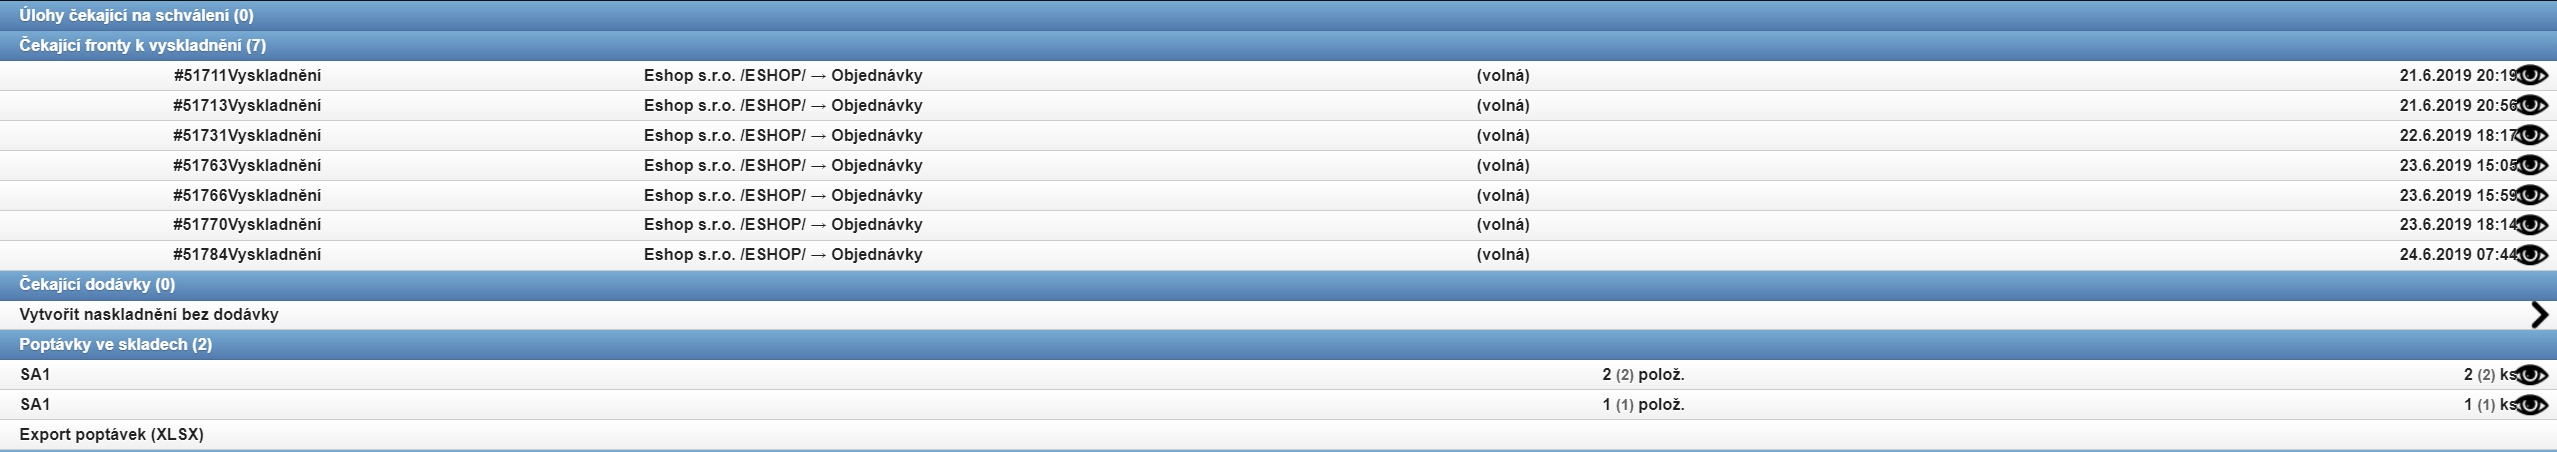
\includegraphics[width=\textwidth]{../png/sysel/vertical.png}
\caption{Ukázka špatné práce s horizontálním místem ve starém skladovém systému} \label{picture:sysel:vertical}
\end{figure}

%%%%%%%%%%%%%%%%%%%%%%%%%%%%%%%%%%%%%%%%%%%%%%%%%%%%%%%%%%%%%%%%%%%%%%%%%%%%%%%%
%%%%%%%%%%%%%%%%%%%%%%%%%%%%%%%%%%%%%%%%%%%%%%%%%%%%%%%%%%%%%%%%%%%%%%%%%%%%%%%%
%%%%%%%%%%%%%%%%%%%%%%%%%%%%%%%%%%%%%%%%%%%%%%%%%%%%%%%%%%%%%%%%%%%%%%%%%%%%%%%%
%%%%%%%%%%%%%%%%%%%%%%%%%%%%%%%%%%%%%%%%%%%%%%%%%%%%%%%%%%%%%%%%%%%%%%%%%%%%%%%%

\section{Analýza konkurence}

Před započetím tvorby nových návrhů UI je vhodné analyzovat existující konkurenční řešení.\\
V dnešní době existuje na trhu nespočet skladových systémů, jednak veřejně dostupných, které nabízejí buď zkušební verzi zdarma, nebo jsou placené, ale zato mají dostupný popis jejich vlastností, a pak také spousta uzavřených systémů, které si nechal někdo vytvořit na míru přesně pro své potřeby, a pro veřejnost není daný systém vůbec dostupný.\\
Z tohoto důvodu jsem se rozhodl zaměřit především na funkcinality veřejně dostupných skladových systémů, které jsou primárně určené na mobilní zařízení.\\

\subsection{Analýza mobilních aplikací pro evidenci skladu}

\subsubsection{Storage Manager: Stock Tracker}

Tuto aplikaci lze nalézt v Google Play Store a je k dispozici její varianta zdarma, kterou jsem také vyzkoušel.\\
Stejně jako Sysel umožňuje skenovat čárové kódy nejen na zboží, ale i na umístění. Má podobné možnosti manipulace se zbožím: naskladnění, vyskladnění, přesun, inventura. Navíc umožňuje pracovat i s objednávkami.\\
Synchronizace probíhá přes úložiště třetí strany (Dropbox, ...) a to vždy pouze při spuštění či ukončení a nebo na přímé vyžádání uživatelem. Jedná se tedy o systém určený především jedné osobě, neboť při použití ve více lidech současně by mohlo docházek ke kolizím v synchronizovaných verzích. Zdá se, že nejsou podporovány ani různé role.\\
Aplikace vůbec nepočítá se systémem “úkolů”. Skladník zde musí sám vědět, co má dělat - nebo informace zjišťovat z jiného systému - nebo pracovat s objednávkami, které systém narozdíl od Sysla podporuje.\\
Naskladnění, vyskladnění a i přesun zboží funguje vždy pouze s jedním typem zboží - nelze hromadně přesunout například celou paletu, na které je různé zboží. U každé položky se znovu vyplňuje celý formulář přesunu.\\

\paragraph{Zajímavé funkcionality:}
\begin{itemize}
	\item Sken čárových kódů běžným fotoaparátem zařízení.
	\item Možnost konfigurace, které prvky se zobrazují na domovské obrazovce.
	\item Možnost konfigurace, které atributy skladových položek či objednávek se mají zobrazovat.
\end{itemize}

\paragraph{Analýza UI:} Jedná se o nativní Android aplikaci, v designu Androidu Jelly Bean. 

\paragraph{Klady UI:}
\begin{itemize}
	\item U pole množství jsou vždy zobrazena \uv{+} a \uv{-} pro usnadnění rychlých změn.
	\item Přepínání aktivních polí formulářů logicky přeskakuje na další, na nových obrazovkách je většinou jako výchozí zvolena položka \emph{EAN}.
	\item Pole výběru data nabízí nativní androidí kalendář.
	\item Přehled provedených transakcí.
	\item V jakýchkoliv seznamech lze vždy hledat, řadit i filtrovat.
	\item V detailu produktu je dole vždy informační proužek zobrazující počet kusů zboží na skladě.
\end{itemize}

\paragraph{Zápory UI:}
\begin{itemize}
	\item Důležité prvky (uložení nového zboží) jsou vždy umístěny v horní liště, která někdy může být špatně dostupná.
	\item Autofocus na některých prvcích neotevírá automaticky klávesnici, je tedy stejně nutné znovu do pole tapnout.
	\item Aplikace nemá menu. Tudíž když se uživatel zanoří hlouběji, musí vícekrát použít tlačítko \emph{zpět}, aby se dostal na domovskou obrazovku.
	\item Při hromadném vyskladňování nelze pracovat \uv{z jednoho místa} - u každého produktu se vždy volí znovu umístění - nezůstává ani předvyplněné.
	\item Celkově se jedná spíše o jednoduchý seznam potřebných informací, UI aplikace není pro uživatele nápomocné ve smyslu navádění, co má být provedeno dále.
\end{itemize}

%%%%%%%%%%%%%%%%%%%%%%%%%%%%%%%%%%%
%%%%%%%%%%%%%%%%%%%%%%%%%%%%%%%%%%%

\subsubsection{Simple Stock Manager}

Tato aplikace je také dostupná na Google Play zdarma, avšak narozdíl od předchozí testované, tato nenabízí možnost zakoupení plné verze a vždy obsahuje reklamy.\\
Nabízí pouze základní funkcionalitu naskladnění a vyskladnění (neumí tedy ani evidovat umístění, zdaleka neumí role, synchronizaci, úkoly, dodací listy, faktury, ...).\\
Provedené transakce lze zpětně upravovat - pro použití této aplikace je to vhodné (je určena pro použití pouze na jednom zařízení), pro nově navrhovaný skladový systém je to funkce nevhodná, neboť je nutné mít přehled o všech pohybech ve skladu - veškerá akce by měla jít vrátit pouze vytvořením nové akce, která bude opakem té první, a obě zůstanou evidovány samostatně.

\paragraph{Zajímavé funkcionality:}
\begin{itemize}
	\item Kalkulačka u polí množství (lze tak efektivně zadat například \uv{5*50 + 7}.
	\item Možnost zobrazení přehledu produktů, kterých je na skladě málo.
\end{itemize}

\paragraph{Analýza UI:} Jedná se o jednoduchou aplikaci, která však má zajímavé funkcionality - nabízí například zajímavé grafy pohybu konkrétního zboží.

\paragraph{Klady UI:}
\begin{itemize}
	\item Při zadávání množství v naskladnění zobrazuje výsledek, kolik bude na skladě po naskladnění.
	\item Má menu, které lze vytáhnout z levého okraje. Uživatel se tak vždy jednoduše dostane tam, kam potřebuje.
	\item Nejvíce potřebné akce jsou na domovské obrazovce dostupné v řádku ve spodní části obrazovky.
	\item V horní části obrazovky je nástřel drobečkové navigace - bohužel ale aplikace nemá více než 1 zanoření a tudíž je její potenciál nevyužitý.
\end{itemize}

\paragraph{Zápory UI:}
\begin{itemize}
	\item Datum se vybírá z vlastního formuláře, který se používá hůře než vestavěný androidí.
	\item Dokončení akce zobrazí vždy potvrzovací dialog, což sice na první pohled může vypadat jako dobrý nápad, ale při přehnaném používání těchto dialogů ztrácí uživatel zájem se nad dialogem rozmýšlet a všechny automaticky potvrzuje, čímž dialog ztrácí smysl \cite{nn-dialogs}.
	\item Chybí auto focus při otevření nových stránek na důležité prvky (vyplnění EAN, hledání…).
	\item Ovládací prvky UI (potrvzení atp.) jsou často malé a špatně se na ně na dotykové obrazovce trefuje.
	\item Z přehledu zboží s nízkou skladovostí lze kliknout na \uv{add} u konkrétního výrobku. Otevře se stránka naskladnění, zvolený výrobek ale není předvyplněn.
	\item Na domovské obrazovce je plovoucí tlačítko pro přidání nového pohybu zboží. Toto tlačítko ale někdy překrývá jiné ovládací prvky, na které není možné kliknout ani při pokusu odscrollovat níže, protože tam už stránka často končí.
	\item Když je menu v levé části vytahováno gestem (posun prstu od kraje obrazovky), je nutné táhnout prst asi až do poloviny obrazovky, jinak se menu neotevře.
	\item V seznamu zboží je pro otevření detailu nutné kliknout na malou akci \uv{Show}, klik na celý řádek produktu nedělá nic.
\end{itemize}

%%%%%%%%%%%%%%%%%%%%%%%%%%%%%%%%%%%
%%%%%%%%%%%%%%%%%%%%%%%%%%%%%%%%%%%

\subsubsection{Vyhodnocení provedené analýzy konkurence.}

K bodům, které jsem v rámci analýzy konkurence sepsal, jsem se následně několikrát vrátil při návrhu a implementaci reálné aplikace, abych neopakoval zde nalezené chyby, nebo naopak zapracoval do svého řešení i nalezené kladné stránky.

\section{Analýza konkurence}

Před započetím tvorby samotných návrhů je potřeba analyzovat konkurenční řešení.\\
V dnešní době existuje na trhu nespočet skladových systémů, jednak veřejně dostupných, které nabízejí například osekanou verzi zdarma, jiné placené, ale s popisem jejich vlastností, a pak také spousta uzavřených systémů, které si nechal někdo vytvořit na míru přesně pro své potřeby, a pro veřejnost není daný systém vůbec dostupný.\\
Z tohoto důvodu jsem se rozhodl zaměřit především na funkcinality veřejně dostupných skladových systémů, které jsou primárně určené na mobilní zařízení.\\

\subsection{Analýza mobilních aplikací pro evidenci skladu}

\subsubsection{Storage Manager: Stock Tracker}

Tuto aplikaci lze nalézt v Google Play Store a je k dispozici její free varianta, kterou jsem také vyzkoušel.\\
Stejně jako Sysel umožňuje skenovat čárové kódy nejen na zboží, ale i na umístění. Má podobné možnosti manipulace se zbožím: naskladnění, vyskladnění, přesun, inventura. Navíc umožňuje pracovat i s objednávkami.\\
Synchronizace probíhá přes úložiště třetí strany (Dropbox…) a to vždy pouze při startu / ukončení a nebo na vyžádání. Jedná se tedy primárně o single-user systém. Zdá se, že nejsou podporovány ani různé role.\\
Aplikace vůbec nepočítá se systémem “úkolů”. Skladník zde musí sám vědět, co má dělat - nebo informace zjišťovat z jiného systému - nebo pracovat s objednávkami, které systém narozdíl od SYSLA podporuje.\\
Naskladnění, vyskladnění a i přesun zboží funguje vždy pouze s jedním typem zboží - nelze hromadně přesunout např celou paletu, na které je různé zboží. U každé položky se znovu vyplňuje celý formulář.\\

\paragraph{Zajímavé funkcionality}
\begin{itemize}
	\item Sken čárových kódů klasickým fotoaparátem zařázení.
	\item Možnost konfigurace, které prvky se na homepage zobrazují.
	\item Možnost konfigurace, které atributy skladových položek, objednávek atp. se zobrazují.
\end{itemize}

\paragraph{Analýza UI} Jedná se o nativní android aplikaci, v designu Androidu Jelly Bean. 

\paragraph{Klady UI}
\begin{itemize}
	\item U pole množství jsou vždy zobrazena + a - pro usnadnění rychlých změn.
	\item Focus na prvcích logicky přeskakuje na další, na nových obrazovkách je většinou jako výchozí zvolen EAN.
	\item Pole výběru data nabízí nativní Androidí kalendář.
	\item Přehled provedených transakcí.
	\item V jakýchkoliv seznamech lze vždy hledat, řadit i filtrovat.
	\item V detailu produktu je dole vždy informační proužek zobrazující, kolik kusů zboží je na skladě.
\end{itemize}

\paragraph{Zápory UI}
\begin{itemize}
	\item Důležité prvky (uložení nového zboží) jsou vždy umístěny v horní liště, která někdy může být špatně dostupná.
	\item Autofocus na některých prvcích neotevírá automaticky klávesnici, je tedy stejně nutné znovu do pole tapnout.
	\item Aplikace nemá menu. Tudíž když se zanořím někam hluboko, musím hodněkrát použít \uv{back}, abych se dostal na domovskou obrazovku.
	\item Při hromadném vyskladňování nelze pracovat \uv{z jednoho místa} - u každého produktu se vždy volí znovu umístění - nezůstává ani nepředvyplněné.
	\item Celkově se jedná spíše o jednoduchý seznam potřebných informací, UI není nějak extra nápomocné.
\end{itemize}

%%%%%%%%%%%%%%%%%%%%%%%%%%%%%%%%%%%

\subsubsection{Simple Stock Manager}

Tato aplikace je také dostupná na Google Play zdarma, avšak narozdíl od předchozí testované, tato nemá plnou verzi za peníze, ale obsahuje reklamy.\\
Nabízí pouze základní funkcionalitu naskladnění a vyskladnění (neumí tedy ani řešit umístění, zdaleka neumí role, synchronizaci, úkoly, dodací listy, faktury...)\\
Provedené transakce lze zpětně upravovat - pro použití této aplikace je to vhodné (je určena pro single-user použití), pro Sysla je to funkce nevhodná z důvodu kontroly nad stock flow.

\paragraph{Zajímavé funkcionality}
\begin{itemize}
	\item Kalkulačka u polí množství (lze tak efektivně zadat například \uv{5*50 + 7}.
	\item Možnost zobrazení přehledu produktů, kterých je na skladě málo.
\end{itemize}

\paragraph{Analýza UI}
Jedná se o jednoduchou aplikaci, která má ale některé zajímavé funkcionality.\\
Nabízí například zajímavé grafy pohybu konkrétního zboží.

\paragraph{Klady UI}
\begin{itemize}
	\item Při zadávání množství v naskladnění zobrazuje výsledek, kolik bude na skladě po naskladnění.
	\item Má menu, které lze vytáhnout z levého okraje. Jednoduše se tak vždy rychle dostanu tak, kam potřebuji.
	\item Nejvíce potřebné akce jsou na domovské obrazovce dostupné v řádku ve spodní části obrazovky.
	\item V horní části obrazovky je nástřel drobečkové navigace - bohužel ale aplikace nemá více než 1 zanoření a tudíž je nevyužita.
\end{itemize}

\paragraph{Zápory UI}
\begin{itemize}
	\item Datum se vybírá z vlastního formuláře, který se používá hůře než vestavěný androidí.
	\item Dokončení akce zobrazí vždy potvrzovací dialog, což sice na první pohled může vypadat jako dobrý nápad, ale při přehnaném použivání těchto dialogů ztrácí uživatel zájem se nad dialogem rozmýšlet, a všechny automaticky potvrzuje, čímž dialog ztrácí smysl \cite{nn-dialogs}.
	\item Chybí auto focus při otevření nových stránek na důležité prvky (vyplnění EAN, hledání…).
	\item Ovládací prvky UI (potrvzení atp.) jsou často malé a špatně se na ně na dotykové obrazovce strefuje.
	\item Z přehledu zboží s nízkou skladovostí lze kliknout na \uv{add} u konkrétního výrobku. Otevře se stránka naskladnění, zvolený výrobek ale není předvyplněn.
	\item Na domovské obrazovce je plovoucí tlačítko pro přidání nového pohybu zboží. Toto tlačátko ale někdy překrývá jiné ovládací prvky, na které není možné kliknout ani při pokusu odscrollovat níže, protože tam už stránka často končí.
	\item Když je menu v levé části vytahováno gestem (posun prstu od kraje obrazovky), je nutné táhnout prst asi až do polovny obrazovky, jinak se menu neotevře.
	\item V seznamu zboží je pro otevření detailu nutné kliknout na malou akci \uv{Show}, klik na celý řádek produktu nedělá nic.
\end{itemize}

// TODO další konkurence

\chapter{Návrh}

\section{Návrh uživatelského rozhraní}

TODO

%%%%%%%%%%%%%%%%%%%%%%%%%%%%%%%%%%%%%%%%
%%%%%%%%%%%%%%%%%%%%%%%%%%%%%%%%%%%%%%%%

\section{Návrh funkčností aplikace}

TODO

\subsection{Undo}

Undo, neboli možnost vrácení akce, tlačítko \emph{zpět}, \emph{vrátit} či \emph{stornovat}. Tím vším je myšlena možnost odvrátit poslední akci, kterou uživatel v systému provedl. Undo je svým způsobem alternativa potvrzovacím dialogům, u kterých bych se chtěl ještě na chvilku zastavit.

\paragraph{Potvrzovací dialogy} Všichni je známe - modální okna, typicky s otázkou a dvěma akcemi: \emph{opravdu smazat/odeslat/\ldots} a \emph{storno}. Jsou používány tam, kde jejích potvrzení je většinou nevratné a dojde k provedení něčeho důležitého. Co když je ale provádění důležitých akcí stěžejní funkčností systému? V příkladu skladového systému jsou veškeré přesuny zboží, naskladnění, vyskladnění atp. důležité akce, u kterých by si měl skladník zkontrolovat, že realita odpovídá stavu v systému. Potvrzovací dialogy na všech těchto akcích ale mohou uživatele i zdržovat - akce, která je v systému vykonávána s vysokou frekvencí, by neměla stále dokola vyžadovat dvojité potvrzení. Nejen že to bude uživatele zdržovat, ale i samotná četnost zapříčiní, že potvrzovací dialog ztratí svůj účel - uživatel bude zvyklý jej \emph{ihned odkliknout}, aniž by se zamyslel nad tím, zda akci chce opravdu provést. (TODO zdroj?)

\paragraph{Undo} Možnost vrátit akci zpět je svým způsobem volnější než potvrzovací dialog - nezdržuje dvojitým potvrzením, ale v případě nutnosti umožňuje špatné rozhodnutí vrátit. Většinou ale nedává moc času na rozmyšlenou - možnost vrátit akci se typicky zobrazuje pouze několik sekund. Také implementace je často mnohem složitější a vyžaduje řádný návrh a spolupráci prezenční a modelové či datové vrstvy.

Při návrhu \emph{undo tlačítka} pro skladový systém jsme společně s Pavlem Kovářem\footnote{spoluautor celého řešení - zabývá se backendovou částí aplikace} zanalyzovali několik možností:
\begin{enumerate}
	\item \textbf{Fronta ve frontendu:} Frontendu by při provedení akce, která by podporovala undo, požadavek reálně neodeslal, ale uložil by jej k pozdějšímu odeslání - například za 5 sekund. Při kliku na undo by se odložené odeslání akce stornovalo, v opačném případě by se požadavek odeslal buďto po uplynutí stanového doby, nebo před provedením jiné další akce.\\\\
	\emph{Zhodnocení řešení:} Jedná se o nejsnadnější implementaci - nevyžaduje žádné úpravy backendu a vše se řeší pouze na klientských zařízeních. S tím ale přichází i hlavní nedostatky tohoto řešení: Když klient ukončí či ztratí spojení se serverem, požadavek se reálně neodešle, přestože systém hlásí, že je odeslaný. Dále když jiný klient provede stejnou akci, dorazí pak na server obě a druhá nemůže být provedena - je potřeba o tom uživatele informovat a problém řešit. Oba problémy jsou poměrně zásadní, a tak byla tato varianta provedení zavržena.
	\item \textbf{Fronta jako middleware:} Frontend by odesílal požadavky ihned, avšak mezi ním a backendem by existoval ještě prostředník: fronta ke zpracování. Ta by požadavky zachytávala a čekala s jejich reálným odesláním backendu. Chování by bylo podobné, jako kdyby s odesláním čekal frontend v předchozí variantě.\\\\
	\emph{Zhodnocení řešení:} Jedná se o řešením, jak předcházet problémům s potenciální ztrátou připojení. Middleware by sloužil jako fronta pro všechny klienty serveru. Když pak klient ztratí či ukončí připojení, požadavek se provede, neboť middleware jej na backend odešle sám. Při ztrátě připojení by se uživateli, který by chtěl použít undo zobrazí informace o ztrátě připojení a informace, že požadavek již byl proveden a bohužel nemůže být stornován.\\
	I zde ale přetrvává problém se synchronizací mezi více klienty - frontend by musel pro každý požadavek, který šel přes frontu, zpětně kontrolovat, že byl nakonec vykonán bezchybně a případně informovat uživatele. To je nepohodlné, ale na druhou stranu ne zcela nereálné řešení.
	\item \textbf{Fronta v backendu:} Požadavky by se odesílaly na backend ihned, a ten by si sám držel frontu obdržených požadavků, ke kterým ještě může přijít požadavek na undo. Opět po uplynutí doby, nebo přijetí požadavku na potvrzení by se změny reálně provedly a potvrdily.\\\\
	\emph{Zhodnocení řešení:} Třetí řešení je velmi podobné tomu druhému, změnou je, že když si bude frontu udržovat přímo backend, může ten s čekajícími požadavky již počítat při vracení dat jiným klientům (soft lock) - a tím předcházet nekonzistencím v datech: Když uživatel A vyskladní poslední kus výrobku, ale tento požadavek ještě čeká ve frontě, uživateli B se již bude zobrazovat, že je na skladě 0 kusů tohoto výrobků a nemůže ho tak vyskladnit duplicitně.\\
	Problémem tohoto řešení je velmi velká náročnost na zpracování těchto zámků a poměrně vysoká šance na neúmyslné chyby v kódu. Z toho důvodu jsme nakonec tuto variantu také zavrhli.
	\item \textbf{Změnové vektory v backendu:} Frontend by vše odesílal hned, backend by vše ihned zpracovával. Kromě zpracování by ale ukládal i změnové vektory, které by bylo možné zpětně odvolat - provést \emph{rollback}. Změnové vektory jsou technikou často používanou například v databázových strojích - veškeré změny jsou zaznamenávány a posléze je možné vše zpětně přehrát a vrátit tak předchozí stav (TODO zdroj?).\\\\
	\emph{Zhodnocení řešení:} V běžné implementaci tato technika umožňuje navrátit stav \emph{celé databáze}, nikoliv pouze jednoho uživatele. Pokud by tedy chtěl undo použít pouze jeden klient, vrátil by se stav i ostatním uživatelům, které si undo vůbec nepřejí. Pro potřeby undo jednoho klienta by tak musely být provedeny mnohé úpravy, a ty by byly neúměrně náročné vůči výsledku. Z důvodu robustnosti tedy tuto variantu taktéž zavrhujeme.
	\item \textbf{Přímá podpora undo v API:} Backendové metody by nativně podporovaly možnost zavolat na určité akce undo: u vybraných funkcí by byla příbuzná metoda, která by jako parametr přijímala identifikátor zaslaný jako výsledek předchozí akce. Jednotlivé požadavky by tak nebyly nijak zdržovány a vše by se provádělo ihned, a požadavek na vrácení změn by byl zpracován jako zcela nová akce.\\\\
	\emph{Zhodnocení řešení:} Mezi výhody posledního z návrhů patří zejména to, že při něm není potřeba řešit konzistenci dat mezi více klienty, vše je ihned potvrzeno a změny se řeší nezávisle na předchozím požadavku. Nevýhodou je, že to není obecné řešení - je potřeba tyto metody implementovat pro všechny akce, které mají undo podporovat. Opět se ale jedná o reálně použitelné řešení, které bude implementováno pouze tam, kde to dává smysl.
\end{enumerate}

Po zhodnocení všech variant jsem se rozhodli jít prozatím cestou pátého návrhu - přímé podpory pouze u vybraných akcí. Důvodem je i fakt, že ve většině akcí by v systému ani chybu jít udělat \emph{nemělo} - tím jsme se posunuli od potvrzovacího dialogu, přes undo, až po \emph{prevenci chyb}. Například u vyskladnění vidí skladník jasný seznam položek, které má vyskladnit, a pokud nemá vše \emph{napípáno}, systému mu ani úkol dokončit nedovolí. U některých vybraných akcí půjde undo provést, a u zbylých, které vyhodnotím jako důležité a málo časté, kde nepůjde realizovat ani prevence chyb, ani undo, skončím u běžných potvrzovacích dialogů.

%%%%%%%%%%%%%%%%%%%%%%%%%%%%%%%%%%%%%%%%
%%%%%%%%%%%%%%%%%%%%%%%%%%%%%%%%%%%%%%%%

\section{Volba technologie}\label{technology}

Jelikož bude aplikace rozdělena na backend, kterým se zabývá můj kolega Bc.~Pavel Kovář, a frontend, který je předmětem této práce, je žádoucí věnovat jistou část textu volbě vhodné technologie.

\paragraph{Cílová platforma} Aplikace je navrhována s ohledem na hardwarové vybavení skladu, ve kterém bude poprvé nasazována: zdejší skladníci jsou vybaveni mobilními telefony \emph{Zebra TC25BJ}, které disponují OS Android 7.1 a vestavěnou čtečkou čárových kódů. Kromě skladníků by měla být aplikace použitelná také z tabletu či stolního počítače pro účely vedoucích pracovníků. Z důvodu jednoduchosti vývoje,  testování, možností aktualizací a obecně dobré zkušenosti z jiných projektů bylo hned při úvodním návrhu určeno, že aplikace bude tvořena formou webové služby, která bude na klientských zařízeních zobrazována ve WebView v jednoduchém kontejneru chovajícím se jako nativní aplikace. Řídící pracovníci budou naopak moci využít přístupu odkudkoliv, kde budou připojeni k internetu pouze pomocí běžného webového prohlížeče.\\
Z tohoto důvodu jsou v následující rešerši zhodnocovány frameworky či knihovny, které usnadňují vývoj \emph{webových aplikací}.

\paragraph{Frameworky a knihovny} V době psaní této práce patří mezi nejpopulárnější \cite{frameworks-github} \cite{frameworks-hackr} front-endové frameworky či knihovny Angular \cite{angular}, React \cite{react}, Vue.js \cite{vue}, Ember.js \cite{ember} a Backbone.js \cite{backbone}.

\paragraph{Názvosloví} Pro účely tohoto textu budu na následujících řádcích používat slovo \emph{framework}, kterým budu označovat jak frameworky, tak knihovny, z důvodu snížení opakování textu.\\

%%%%%%%%%%%%%%%%%%%%%%%%%%%%%%%%%%%%%%%%
%%%%%%%%%%%%%%%%%%%%%%%%%%%%%%%%%%%%%%%%

\subsection{Datum vydání}

Zatímco v současnosti nejčastěji porovnávanými frameworky jsou první dva zmíněné, Vue.js je z této pětice vybraných nejmladší, nabírá ale velké obliby. Ember.js a Backbone.js jsou poté lehce upozaděny z důvodu jejich stáří. Přehled prvního vydání jednotlivých frameworků je v tabulce \ref{table:compare:release}

\begin{table}[h]
\caption{Volba frameworku: Datum vydání}
\label{table:compare:release}
\begin{tabular}{lrrrrr}
\hline
                                         & Angular                     & React                     & Vue.js                     & Ember.js                     & Backbone.js               \\ \hline
Vydání první verze                       & 2010/2016\footnote{V roce 2010 byl vydán AngularJS, který byl v roce 2016 kompletně přepsán do TypeScriptu a vydán jako Angular 2, či jednoduše \emph{Angular}.}                                                                       & 2013                      & 2014                       & 2011                         & 2010                      \\
\end{tabular}
\end{table}

Datum vydání ovšem nelze objektivně ohodnotit bodovým ziskem. Na jedné straně stojí fakt, že starší framework může být vyspělejší a tudíž stabilnější atp., na straně druhé nové frameworky se často učí z chyb provedených jejich předchůdci a vyberou z nich pouze to nejlepší. Tato tabulka tedy zůstane čistě přehledová.

%%%%%%%%%%%%%%%%%%%%%%%%%%%%%%%%%%%%%%%%
%%%%%%%%%%%%%%%%%%%%%%%%%%%%%%%%%%%%%%%%

\subsection{Zázemí}

Zatímco Angular a React jsou vyvíjeny velkými společnostmi: Googlem, respektive Facebookem, které zná každý, Ember.js je vyvíjen společností Tilde Inc. \cite{tilde}, která také není žádným startupem. Vue.js a Backbone.js by se naopak daly nazvat \emph{komunitními projekty}, neboť jsou vytvořeny převážně jedním autorem (Evan You, respektive Jeremy Ashkenas) a rozvíjeny a udržovány komunitou vývojářů. 
\\
Na první pohled by se mohlo zdát, že z tohoto hodnocení budou vycházet lépe ty frameworky, které mají za sebou stabilní firmy, neboť je tím zajištěn jejich kontinuální vývoj. Ve skutečnosti ale velké firmy \emph{zabíjejí} své projekty poměrně často, stačí se podívat například na seznam projektů, které ukončil Google \cite{killed_by_google}. Oproti tomu komunitní projekty mohou žít dále i v případě, že jejich hlavní autor už na projektu nechce, nebo nemůže pracovat. Z toho důvodu nelze jednoznačně určit, které zázemí je pro budoucnost frameworku výhodnější, a u tabulky \ref{table:compare:background} se tedy opět zdržuji udělování bodů.

\begin{table}[h]
\caption{Volba frameworku: Zázemí}
\label{table:compare:background}
\begin{tabular}{lrrrrr}
\hline
                                         & Angular                     & React                     & Vue.js                     & Ember.js                     & Backbone.js               \\ \hline
Zázemí velké\\společnosti                & ano                         & ano                       & ne                         & částečně                     & ne                        \\
\end{tabular}
\end{table}

%%%%%%%%%%%%%%%%%%%%%%%%%%%%%%%%%%%%%%%%
%%%%%%%%%%%%%%%%%%%%%%%%%%%%%%%%%%%%%%%%

\subsection{Licence}

Licence k použití frameworku je důležitá položka při rozhodování. Naštěstí všech 5 porovnávaných frameworků je v době psaní této licencováno pod MIT licencí, která povoluje jakékoliv použití i v komerční sféře, úpravy, distribuce i použití v ne-opensource projektech. Nevýhodou této licence je nulová záruka funkčnosti či zodpovědnost autorů za potenciální spáchané škody tímto softwarem.
\\
\paragraph{Licencování Reactu} Facebook původně vydal svůj React pod BSD licencí spolu s dalšími patenty, avšak 24. září 2017 byl React převeden pod MIT licenci \cite{react-license-commit, react-license}.
\\
Jelikož jsou všechny frameworky licencovány stejně, neprobíhá v tabulce \ref{table:compare:license} žádné bodování.

\begin{table}[h]
\caption{Volba frameworku: Licence}
\label{table:compare:license}
\begin{tabular}{lrrrrr}
\hline
                                         & Angular                     & React                     & Vue.js                     & Ember.js                     & Backbone.js               \\ \hline
Licence                                  & MIT                         & MIT                       & MIT                        & MIT                          & MIT                       \\
\end{tabular}
\end{table}

%%%%%%%%%%%%%%%%%%%%%%%%%%%%%%%%%%%%%%%%
%%%%%%%%%%%%%%%%%%%%%%%%%%%%%%%%%%%%%%%%

\subsection{Křivka učení}

Složitost frameworku je důležitá metrika, neboť má dopady zejména na ekonomickou stránku projektu. Jednoduché prvotní vniknutí do problematiky frameworku ovšem také nemusí být nutně výhodou, pokud v něm je později problémové provést některé pokročilé věci, nebo i v pokročilém stádiu zdržuje svým nízkoúrovňovým přístupem k problémům, které jiné frameworky řeší automaticky.

\paragraph{Angular, React a Vue.js} Přehled obtížnosti tří v současnosti nejčastěji skloňovaných frameworků přehledně shrnul Rajdeep Chandra ve své prezentaci \emph{My experience with Angular 2 , React and Vue} \cite{frameworks-3compare}, ze které vychází hodnocení v tabulce \ref{table:compare:difficulty}.

\paragraph{Ember.js} Tento framework je dle V. Lascika \cite{ember-diffuculty} vhodný spíše pro projekty, na kterých pracuje velké množství vývojářů, a to z důvodu své komplexnosti. Proto jej pro použití v mé vznikající aplikaci hodnotím nula body.

\paragraph{Backbone.js} U této knihovny je důležité zmínit, že umožňuje vývojáři vytvořit si strukturu aplikace kompletně dle svého uvážení \cite{frameworks-rubygarage}. To ssebou může nést jak výhody pro zkušeného, tak nevýhody pro nezkušeného vývojáře, který v pokročilém stádiu vývoje může zjistit, že některou ze základních struktur navrhl špatně. Samotná obtížnost práce s touto knihovnou je ale poměrně nízká.

\begin{table}[h]
\caption{Volba frameworku: Obtížnost}
\label{table:compare:difficulty}
\begin{tabular}{lrrrrr}
\hline
                                         & Angular                     & React                     & Vue.js                     & Ember.js                     & Backbone.js               \\ \hline
Obtížnost                                & vysoká                      & vyšší                     & nízká                      & velmi vysoká\footnote{za předpokladu, že na projektu bude pracovat pouze velmi malé množství vývojářů}                                                                                                                                  & nízká                     \\
\makecell[r]{\textit{bodový zisk}}       & \textit{1}                  & \textit{2}                & \textit{4}                 & \textit{1}                   & \textit{4}                  
\end{tabular}
\end{table}

%%%%%%%%%%%%%%%%%%%%%%%%%%%%%%%%%%%%%%%%
%%%%%%%%%%%%%%%%%%%%%%%%%%%%%%%%%%%%%%%%

\subsection{Oficiální dokumentace}

Hlavním zdrojem ke studiu frameworku by měla být jeho oficiální dokumentace, v této sekci tedy budu hodnotit kvalitu a obsáhlost oficiálního manuálu k jednotlivým frameworkům.

\paragraph{Angular} Jedná se o velmi obsáhlou a dobře rozdělenou dokumentaci \cite{angular-doc}, která obsahuje i řadu příkladů a ve srozumitelné stromové struktuře vývojář jednoduše najde, co potřebuje.

\paragraph{React} Dokumentace Reactu \cite{react-doc} je o poznání jednodušší než ta Angularu, avšak to je způsobeno tím, že React je pouze knihovna, kdežto Angular je plnohodnotný framework. Dokumentace je rozdělena na jednodušší úvod a pokročilejší techniky, je tedy snadné s ní pracovat.

\paragraph{Vue.js} Nejmladší z frameworků má také velmi přátelskou dokumentaci \cite{vue-doc}, která je podobně jako u Angularu velmi bohatá a stromově strukturovaná.

\paragraph{Ember.js} Oficiální manuál Ember.js \cite{ember-doc} je taktéž poměrně obsáhlý a strukturou připomíná dokumentaci Angularu a Vue.js. Obsahuje velké množství ukázek kódu a je logicky strukturován.

\paragraph{Backbone.js} Poslední ze zkoumaných frameworků má oficiální dokumentaci \cite{backbone-doc} na první pohled méně atraktivní a pro nováčka může být matoucí. Oproti ostatním dokumentacím chybí například barevné zvýraznění důležitých bodů a další grafické strukturování textu.

\begin{table}[h]
\caption{Volba frameworku: Dokumentace}
\label{table:compare:docs}
\begin{tabular}{lrrrrr}
\hline
                                         & Angular                     & React                     & Vue.js                     & Ember.js                     & Backbone.js               \\ \hline
\makecell{Kvalita oficiální\\dokumentace} & \makecell{velmi\\vysoká}   & vysoká                    & \makecell{velmi\\vysoká}   & \makecell{velmi\\vysoká}     & střední                   \\
\makecell[r]{\textit{bodový zisk}}       & \textit{3}                  & \textit{2}                & \textit{3}                 & \textit{3}                   & \textit{1}                  
\end{tabular}
\end{table}

%%%%%%%%%%%%%%%%%%%%%%%%%%%%%%%%%%%%%%%%
%%%%%%%%%%%%%%%%%%%%%%%%%%%%%%%%%%%%%%%%

\subsection{Testování}

Testování je při vývoji softwaru velkým tématem. Mnoho vývojářů nerado testuje, jiní se naopak specializují pouze na testování. V moderních aplikacích je testování z větší části řešeno automatizovanými testy, které se spouští v rámci CI. Přestože se tato práce zabývá pouze frontendem, i ten je možné testovat již od úrovně Unit testů, vyvíjej jej pomocí TDD a nakonec samozřejmě vše zkontrolovat pomocí E2E testů.

\paragraph{Angular} Nejkomplexější z frameworků nabízí přehlednou dokumentaci \cite{angular-test}, jak by měl být testován. Popisuje jak používat Unit testy i E2E testy a pro druhý zmíněný typ nabízí i samotný testovací framework: Protractor \cite{protractor}. Jeho testovatelnost tedy hodnotím jako velmi dobrou.

\paragraph{React} Tato knihovna ve své dokumentaci na první pohled testování příliš neprosazuje, avšak stránku dedikovanou této kratochvíli \cite{react-test} lze nakonec také nalézt. Narozdíl od Angularu zde není poskytován dedikovaný framework určený přímo pro testování této knihovny. Stránka popisuje testovací frameworky, které používají různé společnosti: autoři Reactu - Facebook - zmiňují svůj Jest \cite{jest}, také je ale zmiňován Enzyme \cite{enzyme} od Airbnb. Konkrétní příklady použití bychom tedy dále hledali v dokumentacích těchto frameworků. Celkově je pro React k dispozici více různých testovacích frameworků, které opět pokrývají jak Unit, tak E2E testování.

\paragraph{Vue.js} Ani Vue.js se neztratí co se Unit a E2E testů týká. Přímo ve své dokumentaci \cite{vue-test} popisuje spouštění Unit testů pomoci vestavěných příkazů, které interně používají buďto již zmiňovaný Jest nebo Mocha \cite{mocha}, a dále odkazuje na vlastní kompletní testovací knihovnu \cite{vue-test-utils}. Také je možné použít velké množství různých testových frameworků a aplikace ve Vue.js lze vyvíjet i pomocí TDD \cite{vue-tdd}.

\paragraph{Ember.js} Tento framework se ve své dokumentaci věnuje testování poměrně intenzivně a zasvětil mu rovnou několik stránek \cite{ember-test}. Jako výchozí testovací framework představuje vlastní QUnit, avšak informuje, že je možné použít i frameworky třetích stran. Testování přehledně rozděluje na \emph{Unit}, \emph{Container}, \emph{Render}, a \emph{Application} testy a také popisuje jak testovat jednotlivé komponenty. Testování Ember.js tedy také hodnotím jako velmi dobré.

\paragraph{Backbone.js} U posledního zkoumaného frameworku na první pohled není testování moc jasné. Oficiální stránka odkazuje na \emph{test suite} \cite{backbone-test}, což je ovšem stránka, která testy \emph{spouští} a ne popisuje. Zdá se, že na této stránce je možné otestovat svůj prohlížeč, zda podporuje veškeré funkcionality Backbone.js. Co se psaní testů týká, rozumněji již vypadá externí stránka \emph{Backbone.js Testing} \cite{backbone-testing}, která již zmiňuje i zde dříve probírané frameworky jako \emph{Mocha}. Ve výsledku tak bude pravděpodobně testování Backbone vypadat obdobně jako u ostatních frameworků, avšak přístup oficiální dokumentace snižuje jeho pochopení.

\begin{table}[h]
\caption{Volba frameworku: Testování}
\label{table:compare:tests}
\begin{tabular}{lrrrrr}
\hline
                                         & Angular                     & React                     & Vue.js                     & Ember.js                     & Backbone.js               \\ \hline
\makecell[l]{Možnosti testování\\a jejich popis\\v dokumentaci} &\makecell[l]{velmi\\kvalitní} &\makecell[l]{velmi\\kvalitní} &\makecell[l]{velmi\\kvalitní} &\makecell[l]{velmi\\kvalitní} &matoucí \\
\makecell[r]{\textit{bodový zisk}}       & \textit{2}                  & \textit{2}                & \textit{2}                 & \textit{2}                   & \textit{1}                  
\end{tabular}
\end{table}

%%%%%%%%%%%%%%%%%%%%%%%%%%%%%%%%%%%%%%%%
%%%%%%%%%%%%%%%%%%%%%%%%%%%%%%%%%%%%%%%%

\subsection{Vývojářské nástroje}

Dalším důležitým nástrojem při práci s frameworkem je možnost jeho debuggování. Framework by měl nabízet vlastní řešení, které vývojáři usnadní nalézt chybu, zjistit, jak se jeho kód chová či odladil rychlostní problémy.
\\
Všechny ze zde porovnávaných frameworků nabízejí tyto nástroje formou doplňku do prohlížeče, konkrétně se dále budeme bavit o doplňcích pro Google Chrome.

\begin{table}[h]
\caption{Volba frameworku: Devtools}
\label{table:compare:devtools}
\begin{tabular}{lrrrrr}
\hline
                                         & Angular                     & React                     & Vue.js                     & Ember.js                     & Backbone.js               \\ \hline
Název                                    & Augury    & \makecell[r]{React\\Developer\\Tools} & \makecell[r]{Vue.js\\devtools} & \makecell[r]{Ember\\inspector} & \makecell[r]{Backbone\\Debugger} \\
Počet stažení\footnote{Stav k 24. 12. 2018}  & 230k                    & 1.351k                    & 706k                       & 57k                          & 9,5k                      \\
\makecell[r]{\textit{bodový zisk}}       & \textit{2}                  & \textit{4}                & \textit{3}                 & \textit{1}                   & \textit{0}                \\
Hodnocení (z 5)                          & 3.9                         & 4.2                       & 4.7                        & 4.8                          & 4,5                       \\
\makecell[r]{\textit{bodový zisk}}       & \textit{2}                  & \textit{1}                & \textit{3}                 & \textit{4}                   & \textit{2}                  
\end{tabular}
\end{table}

%%%%%%%%%%%%%%%%%%%%%%%%%%%%%%%%%%%%%%%%
%%%%%%%%%%%%%%%%%%%%%%%%%%%%%%%%%%%%%%%%

\subsection{Počet hvězdiček na GitHubu}

Počet hvězdiček na GitHubu lze velmi volně interpretovat jako oblíbenost frameworku mezi vývojáři. Z tohoto důvodu již v tabulce \ref{table:compare:github_stars} hodnotím frameworky dle počtu získaných hvězdiček.

\begin{table}[H]
\caption{Volba frameworku: Počet hvězdiček na GitHubu}
\label{table:compare:github_stars}
\begin{tabular}{lrrrrr}
\hline
                                         & Angular                     & React                     & Vue.js                     & Ember.js                     & Backbone.js               \\ \hline
Počet hvězdiček\\na GitHubu\footnote{Stav k 17. 12. 2018} &   43,6k    & 117,7k                    & 122,3k                     & 20,3k                        & 27,3k                     \\
\makecell[r]{\textit{bodový zisk}\footnote{Hodnocení přeskakuje bodový zisk 3, aby bylo zhodnoceno i absolutní množství hvězdiček, nejen pořadí.}}
                                         & \textit{2}                  & \textit{4}                & \textit{5}                 & \textit{0}                   & \textit{1}                  
\end{tabular}
\end{table}

%%%%%%%%%%%%%%%%%%%%%%%%%%%%%%%%%%%%%%%%
%%%%%%%%%%%%%%%%%%%%%%%%%%%%%%%%%%%%%%%%

\subsection{Počet npm balíků}

Npm \cite{npm} je repozitář javascriptových komponent, na kterém jsou sdíleny jednak kompletní řešení (jako například Angular, Rect, Vue.js a další), ale především různé rozšiřující pluginy do těchto frameworků. Z toho důvodu budu v následující metrice hodnotit, kolik balíků npm nabízí pro jednotlivé porovnávané frameworky.
\\
Bodové zisky hrubě odpovídají relativnímu počtu nalezených balíků.

\begin{table}[h]
\caption{Volba frameworku: Počet npm balíků}
\label{table:compare:npm}
\begin{tabular}{lrrrrr}
\hline
                                         & Angular                     & React                     & Vue.js                     & Ember.js                     & Backbone.js               \\ \hline
Počet npm balíků                         & 26,6k                       & 73,4k                     & 20,6k                      & 6,4k                         & 1,5k                      \\
\makecell[r]{\textit{bodový zisk}}       & \textit{2}                  & \textit{3}                & \textit{2}                 & \textit{1}                   & \textit{0}                 
\end{tabular}
\end{table}

%%%%%%%%%%%%%%%%%%%%%%%%%%%%%%%%%%%%%%%%
%%%%%%%%%%%%%%%%%%%%%%%%%%%%%%%%%%%%%%%%

\subsection{Otázky na Stack Overflow}

Stack Overflow je jedním z portálů sítě Stack Exchange, který zná prakticky každý vývojář. Kdokoliv zde může položit otázku a komunita poté odpovídá, zatímco hlasuje o kvalitě odpovědí, aby byla vybrána ta nejlepší.\\
Z pohledu volby frameworku může být na jednu stranu vhodné, aby bylo na této stránce hodně otázek týkajících se dané technologie, na druhou stranu to ale může znamenat i nekvalitní dokumentaci. Jelikož ale v předchozí sekci nebyla žádná dokumentace vyhodnocena jako vysloveně špatná, budu dále usuzovat, že větší množství otázek je lepší.

\begin{table}[h]
\caption{Volba frameworku: Otázky na Stack Overflow}
\label{table:compare:stackoverflow}
\begin{tabular}{lrrrrr}
\hline
                                         & Angular                     & React                     & Vue.js                     & Ember.js                     & Backbone.js               \\ \hline
\makecell[l]{Počet otázek\\na Stack Overflow} & 146k                   & 118k                      & 28k                        & 23k                          & 21k                       \\
\makecell[l]{Počet \emph{zodpovězených}\\otázek} & 86k                 & 72k                       & 18k                        & 17k                          & 16k                       \\
\makecell[r]{\textit{bodový zisk}}       & \textit{3}                  & \textit{3}                & \textit{1}                 & \textit{1}                   & \textit{1}                  
\end{tabular}
\end{table}

%%%%%%%%%%%%%%%%%%%%%%%%%%%%%%%%%%%%%%%%
%%%%%%%%%%%%%%%%%%%%%%%%%%%%%%%%%%%%%%%%

\subsection{Firemní stack}

Další zvolenou metrikou je, jak daná technologie zapadá do firemní stacku firmy Jagu s.r.o., ve které bude tento nový projekt realizován. Firma se specializuje především na webové aplikace a middlewary na zakázku \cite{jaguweb}, a mezi nejpoužívanější technologie patří PHP (Nette, Laravel, Symfony), dále provozuje jeden informační systém postavený na Angularu a nově také menší aplikaci ve Vue.js. Tabulka \ref{table:compare:stack} shrnuje, jak jsou jednotlivé frameworky blízko k tomuto stacku.

\begin{table}[h]
\caption{Volba frameworku: Shoda s firemním stackem}
\label{table:compare:stack}
\begin{tabular}{lrrrrr}
\hline
                                          & Angular                     & React                     & Vue.js                     & Ember.js                     & Backbone.js               \\ \hline
Shoda s\\firemním stackem                 & ano                         & ne                        & ano                        & ne                           & ne                        \\
\makecell[r]{\textit{bodový zisk}}        & \textit{2}                  & \textit{0}                & \textit{2}                 & \textit{0}                   & \textit{0}                  
\end{tabular}
\end{table}

%%%%%%%%%%%%%%%%%%%%%%%%%%%%%%%%%%%%%%%%
%%%%%%%%%%%%%%%%%%%%%%%%%%%%%%%%%%%%%%%%

\subsection{Dostupnost vývojářů}

Metrikou, kterou z hlediska udržitelnosti projektu a jeho ekonomických nákladů nelze opomenout, je dostupnost a cena vývojářů se zájmem o danou technologii.
\\
Tato data se ale obtížněji získávají, většina statistik hovoří o nabídkách práce v dané technologii, nikoliv o počtu lidí, kteří s ní pracují. Z toho důvodu jsem se rozhodl založit tuto metriku na výsledcích vyhledávání osob v profesní síti LinkedIn - tak dokážeme zjistit alespoň hrubý počet lidí, kteří o sobě sami tvrdí, že jsou vývojáři v daném frameworku.
\\
Bodové zisky zde hrubě reflektují relativní počet nalezených profilů.

\begin{table}[h]
\caption{Volba frameworku: Počet vývojářů na LinkedIn}
\label{table:compare:developers}
\begin{tabular}{lrrrrr}
\hline
                                          & Angular                     & React                     & Vue.js                     & Ember.js                     & Backbone.js               \\ \hline
Počet výsledků\\na dotaz\\"<název> developer"              & 344k       & 333k                      & 78k                        & 21k                          & 76k                       \\
\makecell[r]{\textit{bodový zisk}}        & \textit{4}                  & \textit{4}                & \textit{2}                 & \textit{1}                   & \textit{2}                  
\end{tabular}
\end{table}

%%%%%%%%%%%%%%%%%%%%%%%%%%%%%%%%%%%%%%%%
%%%%%%%%%%%%%%%%%%%%%%%%%%%%%%%%%%%%%%%%

\subsection{Integrace se Sentry}

Sentry \cite{sentry} je nástroj sloužící k automatickému i manuálnímu záznamu chyb v aplikacích. Ve firmě Jagu s.r.o. je využíván v řadě projektů a jeho nasazení bude vhodné i pro aplikaci řešenou v rámci této práce. Z toho důvodu je vhodné se podívat, jak hlubokou integraci je možné mezi jednotlivými frameworky a Sentry realizovat.\\
Při pohledu na přehled toho, jaké technologie Sentry podporuje v JavaScriptu \cite{sentry-js} rychle zjišťujeme, že všech pět zde zkoumaných frameworků je oficiálně podporováno, včetně rychlého návodu na zprovoznění. Z toho důvodu neprobíhá v tabulce \ref{table:compare:sentry} žádné bodování.

\begin{table}[h]
\caption{Volba frameworku: Integrace se Sentry}
\label{table:compare:sentry}
\begin{tabular}{lrrrrr}
\hline
                                         & Angular                     & React                     & Vue.js                     & Ember.js                     & Backbone.js               \\ \hline
\makecell[l]{Oficiální integrace\\se Sentry} & ano                     & ano                       & ano                        & ano                          & ano                       \\
\end{tabular}
\end{table}

%%%%%%%%%%%%%%%%%%%%%%%%%%%%%%%%%%%%%%%%
%%%%%%%%%%%%%%%%%%%%%%%%%%%%%%%%%%%%%%%%

% \subsection{Vybavenost frameworku TODO}

% V poslední části se zaměříme na to, jaké funkce jednotlivé frameworky nabízí, a zda je vhodné jejich použití pro frontend skladového systému, který je předmětem této práce. Jelikož systém bude vždy napojen na backend, který bude poskytovat data i bussiness logiku, je vhodné se zamyslet i nad tím, aby framework zbytečně neobsahoval nepotřebné součásti, které by v tomto případě byly spíše na obtíž a zanášely jednoduchou aplikaci zbytečnými složitostmi.

% \paragraph{Angular} Ze všech zde porovnávaných frameworků se jedná o ten nejkomplexnější. Nabízí Dependency Injection, Services, Router, TODO

% \paragraph{React} Tím, že je React pouze knihovna a nikoliv framework, nenabízí tolik součástí jako Angular: neexistuje zde Dependency Injection\footnote{DI je do Reactu možné doplnit pomocí knihoven třetích stran}, Services, Router\footnote{Router je možné doplnit knihovnou}, vše je komponenta.TODO

% \paragraph{Vue.js} Co se nabízených komponent týká, Vue.js stojí mezi Angularem a Reactem. Vue.js je považováno za framework, a samo o sobě říká, že obsahuje \emph{to nejlepší z Angularu}. Například Router je možné použít jak oficiální vestavěný, tak jiný router třetí strany \cite{vue-routers}. Dependency injection je také dostupné jako knihovna třetí strany.TODO

% \paragraph{Ember.js} 

% \paragraph{Backbone.js} Backbone.js je z pěti porovnávaných 

%%%%%%%%%%%%%%%%%%%%%%%%%%%%%%%%%%%%%%%%
%%%%%%%%%%%%%%%%%%%%%%%%%%%%%%%%%%%%%%%%

\subsection{Souhrn průzkumu}

V tabulce \ref{table:compare:results} jsou sečteny body z předchozích dílčích hodnocení.

\begin{table}[h]
\caption{Volba frameworku: Výsledky}
\label{table:compare:results}
\begin{tabular}{lrrrrr}
\hline
                                          & Angular                     & React                     & Vue.js                     & Ember.js                     & Backbone.js               \\ \hline
\makecell[r]{bodový zisk celkem}          & 23                          & 25                        & 27                         & 14                           & 12                  
\end{tabular}
\end{table}

Výsledky rozdělují frameworky na dvě skupiny. V té vedoucí je trojice Angular, React a Vue.js, v pozadí poté zůstávají Ember.js a Backbone.js. Na tomto místě je také vhodné znovu zmínit, že hodnocení frameworků probíhalo ve vztahu ke konkrétnímu projektu, který je cílem této práce, a také ve vztahu k firmě Jagu~s.r.o., která vývoj této aplikace zaštiťuje.\\
První tři frameworky jsou seřazeny poměrně těsně za sebou, avšak nejlépe vyšel ze srovnání nejmladší Vue.js, který tímto volím jako framework, ve kterém budu na práci dále pracovat.


\chapter{Implementace}\label{implementation}

V této kapitole se budu věnovat převážně některým obecným součástem aplikace a jak jsem došel k jejich výsledné podobě. Obsahem \emph{není} popis realizace funkčních požadavků aplikace, přestože jsem jejich implementaci strávil nezanedbatelné množství času. Tento popis je již totiž dostupný ve formě analýzy a návrhu, kterým odpovídá.\\

%%%%%%%%%%%%%%%%%%%%%%%%%%%%%%%%%%%%%%%%%%%%%%%%%%%%%%%%%%%%%%%%%%%%%%%%%%%%%%%%
%%%%%%%%%%%%%%%%%%%%%%%%%%%%%%%%%%%%%%%%%%%%%%%%%%%%%%%%%%%%%%%%%%%%%%%%%%%%%%%%
%%%%%%%%%%%%%%%%%%%%%%%%%%%%%%%%%%%%%%%%%%%%%%%%%%%%%%%%%%%%%%%%%%%%%%%%%%%%%%%%
%%%%%%%%%%%%%%%%%%%%%%%%%%%%%%%%%%%%%%%%%%%%%%%%%%%%%%%%%%%%%%%%%%%%%%%%%%%%%%%%

\section{Podpůrné nástroje vývoje}

\subsection{Webpack}

Webpack \cite{webpack} je software, který zpracovává součásti webových aplikací a tvoří z nich balíčky vhodné pro webové prohlížeče. Primárně je zaměřen na Javascript, ale dokáže zpracovávat i řadu dalších formátů, přes styly v css, sass či stylus, obrázky v png, jpg, svg, ale také konfigurace v json, yaml a dalších.\\
Hlavním důvodem, proč používat Webpack, je možnost rozdělování kódu do jednotlivých souborů. Při programování je pohodlné mít oddělené ucelené komponenty, různé konfigurační soubory apod. Výstupem webpacku jsou poté typicky pouze čtyři soubory: dva obsahující logiku aplikace (.js) a dva pro stylování (.css), přičemž logika i styly jsou rozděleny na samotnou aplikaci - kód programátora, a kód třetích stran - tzv. \code{vendor}.

\paragraph{Použití loaderů.} Další příležitost k použití webpacku přichází ve chvíli, kdy chceme v projektu mít kód, který není v cílovém prohlížeči podporován. Tím může být například SASS, nebo třeba i moderní syntaxe Javascriptu řídící se standardem ES6 či novějším. S pomocí Webpacku lze nastavit, aby se při zpracování některých souborů použil \emph{loader}, který například převede SASS na CSS, konstrukce ES6 na ES5 apod. \cite{webpack-ackee}.

\paragraph{Webpack ve spolupráci s Vue.js.} Konfigurace webpacku může být pro neznalého uživatele až příliš obsáhlá a může být jednoduché v ní udělat chybu, kvůli které bude například výsledný build aplikace neoptimalizovaný a tudíž pomalý. Vývojáři Vue tento problém mitigovali tak, že celá optimalizovaná konfigurace webpacku je součástí \code{vue-cli}, což znamená, že stačí mít v projektu jako závislosti právě tento npm modul, a pokud nejsou vyžadovány žádné pokročilé funkce, funguje vše \emph{automagicky}\footnote{Nejedná se o překlep, jde o spojení slov automaticky a magicky}. Pro účely porovnání jsem se podíval, jak dlouhá je konfigurace webpacku, kterou má Vue automaticky v sobě - jedná se o \emph{1490 řádků kódu}.

%%%%%%%%%%%%%%%%%%%%%%%%%%%%%%%%%%%%%%%%
%%%%%%%%%%%%%%%%%%%%%%%%%%%%%%%%%%%%%%%%

\subsection{Vue-UI}

V předchozím paragrafu jsem popisoval výhodu použití Vue-CLI, ke kterému je ale vhodné říci i několik dalších slov, jelikož se jedná o velmi prakticky nástroj, usnadňující mnoho běžných požadavků na správu projektu.\\
Zaměřit bych se chtěl především na možnost spuštění grafického prostředí, pomocí \code{vue ui} z terminálu, což si vytvoří vlastní webový server a na adrese \code{localhost:8000} spustí grafickou správu projektu. Ta obsahuje následující možnosti:
\begin{itemize}
    \item \emph{přehled projektů}, který nabízí rychlou kontrolu dostupných aktualizací použitých balíčků, kontrolu bezpečnostních mezer nebo RSS čtečku novinek od Vue komunity,
    \item \emph{instalované pluginy}, což jsou běžné npm balíčky, ke kterým je ale možné přidat další konfiguraci. Jedný se například o pluginy pro samotné \code{vue-cli}, \code{eslint} nebo třeba knihovnu \code{vuetify}, která poskytuje grafické komponenty, a pomocí tohoto pluginu vkládá do výsledného buildu pouze ty, které jsou skutečně v aplikaci používány.
    \item \emph{instalované závislosti}, u kterých je možné jednoduše hromadně aktualizovat na nové verze, zobrazovat, jakou verzi používáme a jaká je nejnovější, nebo přes jednotné hledání instalovat nové závislosti,
    \item \emph{úlohy spouštěné nad kódem aplikace}, asi nejpraktičtější součást Vue-UI, ze které je možné spouštět lokální dev-server ale také build pro produkci. Největší výhodou spouštění těchto úloh z UI je ta, že po skončení úlohy jsou zde dostupné bohaté informace o velikosti výsledných souborů a přehled, jak velká je která závislost. Jako příklad uvedu dále optimalizaci velikosti překladů.
\end{itemize}

\paragraph{Optimalizace velikosti aplikace odebráním zbytečných překladů.} Jednou ze závislostí, kterou v projektu používám, je knihovna \emph{moment} \cite{momentjs}, která se stará o parsování a zobrazování datumů a časů, a jejíž součástí jsou i překlady do 127 jazyků. Jeden soubor s jazykem má sice \uv{pouze} 172 řádků kódu, ale při vzájemném pronásobení to už je \emph{21844 řádků}. Není tak divu, že při analýze velikostu výsledných souborů pomocí Vue-UI jsem odhalil, že tyto překlady zabírají téměř \emph{15\% celé velikosti} souboru s kódem třetích stran (\code{vendor}), jak je znázorněno na obrázku \ref{picture:cli:analyze}.

\begin{figure}[]
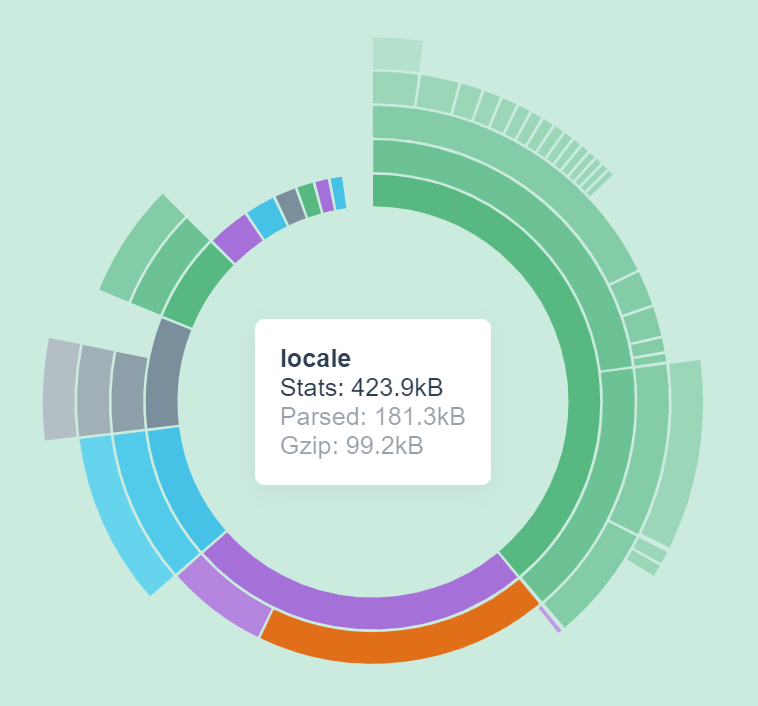
\includegraphics[width=0.7\textwidth]{../png/cli/analyze-moment.png}
\caption[Analýza velikosti výsledné aplikace: překlady moment.js]{Analýza velikosti výsledné aplikace: překlady moment.js (na obrázku popsáno jako locale a označeno oranžově) zabírají velké procento z celkové velikosti souboru.} \label{picture:cli:analyze}
\end{figure}

Našel jsem si tedy řešení spočívající v přidání jednoho řádku konfigurace \cite{momentjs-ignore-locale}, jehož cílem je nezahrnovat do výsledného buildu ty jazyky, které nepoužívám (což jsou všechny, kromě češtiny a angličtiny). Výsledek je takový, že nyní překlady nezabírají \emph{ani jedno celé procento}.

%%%%%%%%%%%%%%%%%%%%%%%%%%%%%%%%%%%%%%%%%%%%%%%%%%%%%%%%%%%%%%%%%%%%%%%%%%%%%%%%
%%%%%%%%%%%%%%%%%%%%%%%%%%%%%%%%%%%%%%%%%%%%%%%%%%%%%%%%%%%%%%%%%%%%%%%%%%%%%%%%
%%%%%%%%%%%%%%%%%%%%%%%%%%%%%%%%%%%%%%%%%%%%%%%%%%%%%%%%%%%%%%%%%%%%%%%%%%%%%%%%
%%%%%%%%%%%%%%%%%%%%%%%%%%%%%%%%%%%%%%%%%%%%%%%%%%%%%%%%%%%%%%%%%%%%%%%%%%%%%%%%

\section{Router}

Jednou z prvních komponent, kterou jsem k čistému Vue.js přidal, byl oficiální Vue Router \cite{vue-router}. Koncept routeru je dobře znám z jakékoliv jiné aplikace, která nějak pracuje s prohlížečem uživatele.\\
Rozdíl Vue.js routeru oproti tomu, který je používán třeba v PHP, spočívá v dynamičnosti celého Javascriptového frameworku: oproti standardním webovým stránkám, kde přesměrování na novou adresu skutečně vyvolá požadavek na server, který odpoví obsahem stránky na dané URL (diagram \ref{picture:route:http}), zde se vše děje dynamicky přímo na klientském zařízení, obsah je vyměněn pomocí Javascriptu a hodnota adresního řádku se změní pouze \uv{pro efekt} - tj. aby uživatel věděl, kde se nachází, a aby mohl adresu zkopírovat a sdílet. Samozřejmě i zde většinou dochází k načítání dat nově otevřené stránky, ale vše je typicky asynchronní - stránka se změní ihned a teprve poté jsou do ní doplněna data - viz diagram \ref{picture:route:vue}.

\begin{figure}[]
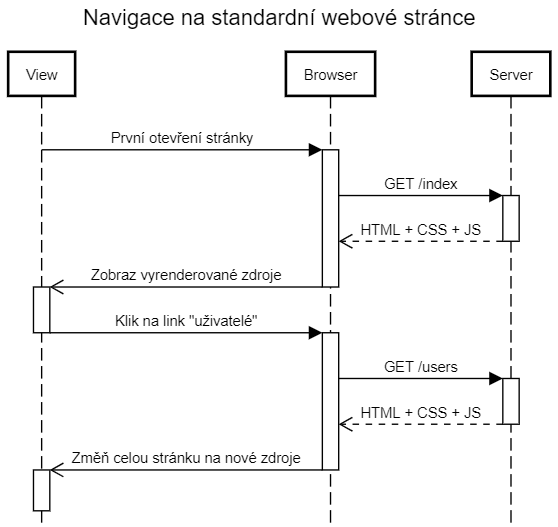
\includegraphics[width=0.7\textwidth]{../png/diagrams/sequence-http-navigate.png}
\caption[Navigace na standardní webové stránce]{Navigace na standardní webové stránce: Pro každý link existuje cesta na serveru, který odpovídá kompletním obsahem této stránky.} \label{picture:route:http}
\end{figure}

\begin{figure}[]
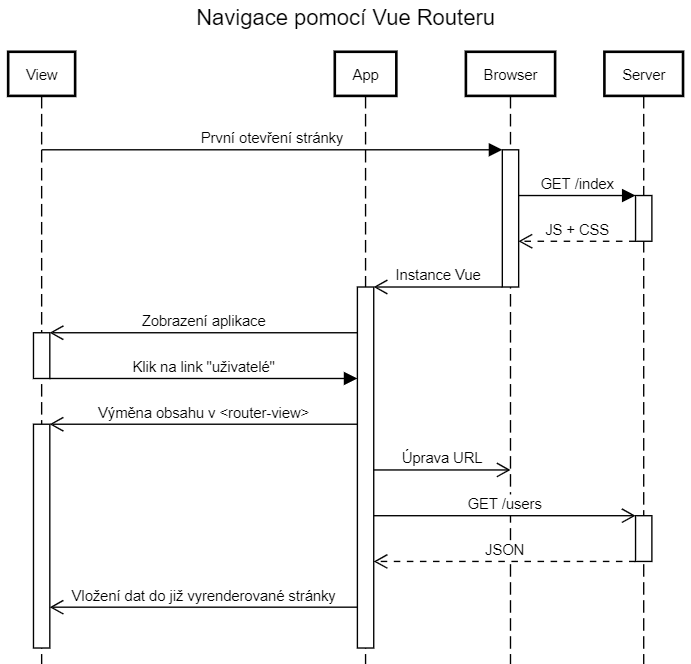
\includegraphics[width=0.9\textwidth]{../png/diagrams/sequence-vue-router.png}
\caption[Navigace v aplikaci pomocí Vue Router]{Navigace v aplikaci pomocí Vue Router: Kompletní obsah aplikace se ze serveru stáhne pouze při prvním přístupu, navigaci v aplikaci řeší Vue Router přímo na klientu a od serveru či jiného API vyžaduje pouze konkrétní data, která v aplikaci zobrazuje.} \label{picture:route:vue}
\end{figure}

% title Navigace na standardní webové stránce

% View->Browser:První otevření stránky
% activate Browser
% Browser->Server:GET /index
% activate Server
% Server-->>Browser:HTML + CSS + JS
% deactivate Server
% Browser->>View:Zobraz vyrenderované zdroje
% deactivate Browser
% activate View


% View->Browser:Klik na link "uživatelé"
% deactivate View
% activate Browser
% Browser->Server:GET /users
% activate Server
% Server-->>Browser:HTML + CSS + JS
% deactivate Server
% Browser->>View:Změň celou stránku na nové zdroje
% deactivate Browser
% activate View


% title Navigace pomocí Vue Routeru
% 
% participant View
% participant App
% participant Browser
% participant Server
% 
% View->Browser:První otevření stránky
% activate Browser
% Browser->Server:GET /index
% activate Server
% Server-->>Browser:JS + CSS
% deactivate Server
% Browser->>App:Instance Vue
% deactivate Browser
% activate App
% App->>View:Zobrazení aplikace
% activate View
% 
% 
% View->App:Klik na link "uživatelé"
% deactivate View
% App->>View:Výměna obsahu v <router-view>
% activate View
% App->>Browser:Úprava URL
% App->>Server:GET /users
% activate Server
% Server-->>App:JSON
% deactivate Server
% App->>View:Vložení dat do již vyrenderované stránky
% 

\paragraph{Titulky stránek.} Lehce matoucí může u tohoto \emph{frontendového routování} být nastavování titulků stránek, tedy \code{<title>} tagů v HTML. Celá aplikace má totiž stále pouze jeden \code{<title>} zapsaný v souboru \code{index.html}, který se sám o sobě při navigaci za pomocí routeru vůbec nemění. K vyřešení tohoto problému sice ve Vue Routeru neexistuje nativní podpora, ale řešení je opravdu snadné - je popsáno v jednom z \emph{issues} v repozitáři na GitHubu \cite{vue-router-title} a spočívá v doplnění titulků do \code{meta} atributů cest, viz ukázka kódu \ref{code:vue-router-title1}, a dále úpravě samotné instance routeru, viz ukázka kódu \ref{code:vue-router-title2}.

\begin{listing}[]
\begin{minted}[linenos,frame=lines]{javascript}
{
    path: '/',
    component: Homepage,
    meta: {
        title: 'Swordfish'
    }
}
\end{minted}
\caption{Nastavování titulků stránek pomocí Vue routeru - úprava definic} \label{code:vue-router-title1}
\end{listing}

\begin{listing}[]
    \begin{minted}[linenos,frame=lines]{javascript}
router.beforeEach((to, from, next) => {
    document.title = to.meta.title;
    next();
})
\end{minted}
\caption{Nastavování titulků stránek pomocí Vue routeru - úprava instance routeru} \label{code:vue-router-title2}
\end{listing}

Toto nastavování titulků stránek jsem nakonec ještě více upravil po svém, jelikož jsem chtěl mít v titulcích i konkrétní hodnoty, které se zobrazují na dané stránce - například při úpravě skladu \emph{Centrální sklad Praha} nechci mít v titulku \uv{Úprava skladu}, ale \uv{Úprava skladu 'Centrální sklad Praha'}. Jelikož jsou ale tyto informace načítány dynamicky až po vstupu na danou stránku (URL stránky může být například \code{/stocks/12/edit} - z té to tedy vyčíst nelze), je nutné i titulek nastavovat dynamicky. Zachoval jsem tedy jako výchozí hodnotu titulku stránky ten, který je nastaven přímo v definici cesty v routeru (ukázka kódu \ref{code:vue-router-title1}), avšak zevnitř komponenty je možné pomocí jednotné funkce titulek obohatit dalšími informacemi - jako například názvem upravované položky.

\paragraph{Drobečková navigace.} Další úpravou routeru, kterou jsem do jisté míry realizoval po svém, je generování drobečkové navigace. Vue Router ve spojení s Vuetify nemají nativní podporu pro zjišťování rodičovských stránek, a tak jsem si lehkou úpravou a vlastní komponentou pro vykreslování \emph{Breadcrumbs} toto zautomatizoval:\\
Každá definovaná routa má nastaveného rodiče, ke kterému poskytuje \emph{getter}. Ve vykreslování drobečkové navigace se poté na aktuální routě zjišťují rekurzivně její rodiče, a včetně jejich parametrů se z nich zpětně tvoří celý strom navigace.\\
Co se na první pohled může zdát jednoduché, se zkomplikuje ve chvíli, kdy chceme mít v cestě parametrizovanou stránku.\\
Například v URL \code{/stocks/1/locations/12/update} je potřeba v definici routy nahradit všechny identifikátory jejich reálnými hodnotami, které ale naštěstí Vue Router poskytuje i během runtime. Funkce pro vytvoření jednoho odkazu, ze kterých se skládá drobečková navigace, je znázorněna v ukázce kódu \ref{code:router:buildPath} - jejími argumenty jsou definice cesty v routě a objekt s aktuálními hodnotami parametrů.

\begin{listing}[H]
    \begin{minted}[linenos,frame=lines]{javascript}
function buildPath(pathWithPlaceholders, parameters) {
    let routePath = pathWithPlaceholders.replace(/\([^/]+\)/g, '');
    const matches = routePath.match(/(:[a-zA-Z]+\/)|(:[a-zA-Z]+$)/g);
    if (matches !== null) {
        for (const match of matches) {
            const matchParam = match.replace(/\//, '').replace(/:/, '');
            routePath = routePath
                        .replace(match, parameters[matchParam] + '/');
        }
    }
    return routePath;
}
\end{minted}
\caption[Automatické generování drobečkové navigace]{Automatické generování drobečkové navigace z definic Vue Routeru, včetně podpory parametrizovaných zanořených cest} \label{code:router:buildPath}
\end{listing}

%%%%%%%%%%%%%%%%%%%%%%%%%%%%%%%%%%%%%%%%%%%%%%%%%%%%%%%%%%%%%%%%%%%%%%%%%%%%%%%%
%%%%%%%%%%%%%%%%%%%%%%%%%%%%%%%%%%%%%%%%%%%%%%%%%%%%%%%%%%%%%%%%%%%%%%%%%%%%%%%%
%%%%%%%%%%%%%%%%%%%%%%%%%%%%%%%%%%%%%%%%%%%%%%%%%%%%%%%%%%%%%%%%%%%%%%%%%%%%%%%%
%%%%%%%%%%%%%%%%%%%%%%%%%%%%%%%%%%%%%%%%%%%%%%%%%%%%%%%%%%%%%%%%%%%%%%%%%%%%%%%%

\section{Moderní webová aplikace}

V kapitole \ref{technology} jsem zmiňoval, že skladník bude aplikaci používat z nativní Android aplikace, která bude obalovat WebView, a vedoucí skladu si aplikaci otevře v běžném browseru - pro obě použití by níže popisovaná konfigurace nebyla potřeba, avšak pokud by někdo nepotřeboval čtečku čárových kódu - což je jediný důvod, proč skladníci používají jako základ nativní Android aplikaci, je možné si otevřít na mobilu běžnou stránku a použít volbu \uv{Přidat na plochu}. Tím vznikne zástupce, který zobrazuje \emph{favicon} webové stránky a po jehož otevření se opět otevře běžný webový prohlížeč.\\
Pokud je však na stránce definovaný \code{manifest.json} pro webové aplikace, může se po otevření tohoto zástupce otevřít stránka v režimu celé obrazovky, a to případně i se skrytými ovládacími prvky - vše tak vypadá, jako kdyby se jednalo o nativní nainstalovanou aplikaci. Základní konfigurace tohoto manifestu je vidět v ukázce kódu \ref{code:webapp-manifest}.

\begin{listing}[H]
\begin{minted}[linenos,frame=lines]{json}
{
  "name": "Swordfish",
  "icons": [
    {
      "src": "favicon/swordfish-192x192.png",
      "sizes": "192x192",
      "type": "image/png"
    },
    {
      "src": "favicon/swordfish-512x512.png",
      "sizes": "512x512",
      "type": "image/png"
    }
  ],
  "start_url": "/",
  "display": "standalone",
  "orientation": "portrait",
  "background_color": "#009688"
}

\end{minted}
\caption{Manifest pro webové aplikace} \label{code:webapp-manifest}
\end{listing}

Tento soubor je vlastně také první krok k vytvoření PWA - Progresivní webové aplikace, což znamená takové webové aplikace, která do jisté míry může fungovat i bez připojení k internetu. Využívá k tomu Service Worker API \cite{service-worker-api}, jehož specifikace je v době psaní tohoto textu stále ve stavu návrhu, přestože vzniká již od května roku 2014 \cite{service-worker-first}.\\
I přes nedokončenou speficikaci se již PWA běžně používají a i ve skladové aplikaci by bylo vhodné toto API využít, to již ale není předmětém této práce a proto jej v tuto chvíli dále nerozvádím.

%%%%%%%%%%%%%%%%%%%%%%%%%%%%%%%%%%%%%%%%%%%%%%%%%%%%%%%%%%%%%%%%%%%%%%%%%%%%%%%%
%%%%%%%%%%%%%%%%%%%%%%%%%%%%%%%%%%%%%%%%%%%%%%%%%%%%%%%%%%%%%%%%%%%%%%%%%%%%%%%%
%%%%%%%%%%%%%%%%%%%%%%%%%%%%%%%%%%%%%%%%%%%%%%%%%%%%%%%%%%%%%%%%%%%%%%%%%%%%%%%%
%%%%%%%%%%%%%%%%%%%%%%%%%%%%%%%%%%%%%%%%%%%%%%%%%%%%%%%%%%%%%%%%%%%%%%%%%%%%%%%%

\section{Překlady}

Novou aplikaci je dnes vhodné hned od počátku psát jako \emph{multijazyčnou} - jako základ tedy například v češtině a angličtině.\\
Pro překlady Vue.js aplikací je vhodné použít knihovnu \code{vue-i18n}\footnote{název je zkratka slova \emph{internationalization} - číslovka 18 značí počet přeskočených znaků} \cite{vue-i18n}, jejíž použití je obdobné, jako známe z jiných jazyků. Zatímco například v PHP se často překlady zapisují do \code{.yaml} nebo \code{.neon}, což jsou formáty, které sice umožňují například zanořování, ale s dalšími funkcemi už si často neporadí, zde se texty zapisují do běžného \code{.js} souboru (ukázka kódu \ref{code:i18n-def}), jehož výstupem je JSON. To znamená, že můžeme používat libovolné konstrukce Javascriptu, od standarního zápisu (klíč \code{close} ve zmiňované ukázce), přes spojování řetězců a používání konstant (podklíče \code{user}), po proměnné klíče (podklíče \code{orderState}), jejichž definice se doplní z číselníku načteného klidně i z jiného souboru. Kreativní autor překladů by jistě našel i prostor pro použití cyklů nebo funkcí, mně ale pro potřeby skladové aplikace stačily znázorněné možností.

\begin{listing}[h]
\begin{minted}[linenos,frame=lines]{js}
const user = "uživatele";

{
    close: "Zavřít",
    user: {
        create: "Vytvořit " + user,
        update: "Upravit " + user
    },
    orderState: {
        [OrderStateEnum.CREATED]: 'Vytvořená',
        [OrderStateEnum.SENT]: 'Odeslaná',
    }
}
\end{minted}
\caption[Definice překladů pro i18n]{Definice překladů pro i18n, včetně pokročilých funkcí jako například spojování řetězců nebo využítí číselníků.} \label{code:i18n-def}
\end{listing}

\paragraph{Překlady a uživatelská nápověda.} Jelikož výsledná aplikace obsahuje i stručnou nápovědu, která má zatím pouze textový obsah, využil jsem pro zápis jejího obsahu také formát, který používá \code{i18n} pro překlady. Tyto texty jsem ale neintegroval do seznamu obecných překladů v aplikaci, ale pracuji s nimi odděleně - pomocí vlastního řešení pro zobrazování nápovědy. Tím mohu všechny texty této \uv{sekce} načíst hromadně a umožnit v nich například vyhledávání, nebo je vkládám přímo k formulářovým atributům, které dokumentují.

%%%%%%%%%%%%%%%%%%%%%%%%%%%%%%%%%%%%%%%%%%%%%%%%%%%%%%%%%%%%%%%%%%%%%%%%%%%%%%%%
%%%%%%%%%%%%%%%%%%%%%%%%%%%%%%%%%%%%%%%%%%%%%%%%%%%%%%%%%%%%%%%%%%%%%%%%%%%%%%%%
%%%%%%%%%%%%%%%%%%%%%%%%%%%%%%%%%%%%%%%%%%%%%%%%%%%%%%%%%%%%%%%%%%%%%%%%%%%%%%%%
%%%%%%%%%%%%%%%%%%%%%%%%%%%%%%%%%%%%%%%%%%%%%%%%%%%%%%%%%%%%%%%%%%%%%%%%%%%%%%%%

\section{State management pattern} \label{impl:vuex}

Jako první se zde sluší říci, co to vlastně \emph{State management pattern} je. Ve Vue.js aplikaci máme typicky velké množství komponent, které mezi sebou často potřebují sdílet nějaký \emph{stav}. Nabízí se tedy vytvoření centrálního bodu, který bude stav udržovat, a umožní jej měnit. Na změny by v ideálním případě měly dotčené komponenty reagovat automaticky, a tyto změny by také měly být nějak řízeny, aby nebylo možné nastavit nevalidní hodnoty. Přesně toto nabízí knihovna \emph{Vuex} \cite{vuex}, jejíž interní cyklus popisuje diagram \ref{picture:vuex}.

\begin{figure}[]
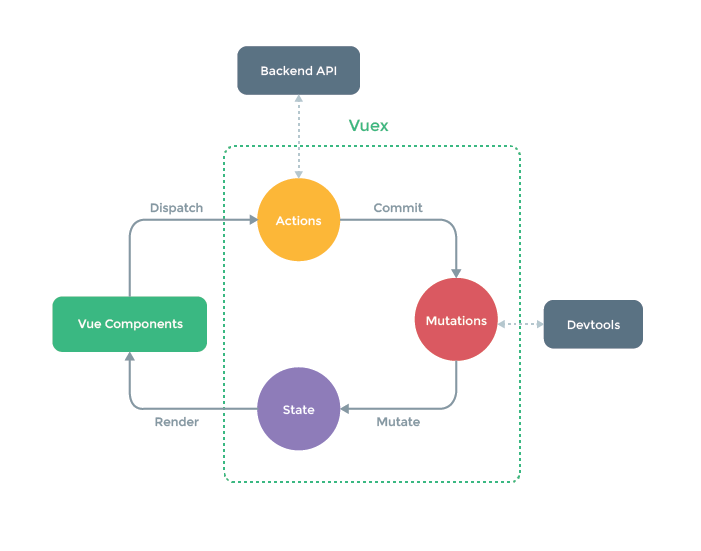
\includegraphics[width=\textwidth]{../png/diagrams/vuex.png}
\caption{Diagram použití Vuex}\label{picture:vuex}
\end{figure}

Nebudu zde rozepisovat detaily jejího použití, ty jsou dostupné kdykoliv online v její kvalitní dokumentaci. Popíšu ale mé vlastní zkušenosti s touto knihovnou, a jak jsem implementoval některá vylepšení. Začněme však od kraje - jako první jsem Vuex použil pro zobrazování snack message - tedy krátkých informačních zpráv, které se zobrazují uživateli ve spodní části obrazovky, především jako potvrzení jeho akce. K tomu jsem použil Vuex do jehož stavu jsem ukládat obsah zprávy a případně její trvání. Ukázku zaslání takové zprávy znázorňuje ukázka kódu \ref{code:vuex-snack-use}.

\begin{listing}[h]
\begin{minted}[linenos,frame=lines]{js}
this.$store.dispatch('snackbar/setSnack', '<message to display>');
\end{minted}
\caption{Vuex pro snackbar-message: použití z jiné komponenty} \label{code:vuex-snack-use}
\end{listing}

Výše uvedený kód se mi ovšem v průběhu psaní aplikace přestal líbit, neboť zobrazování těchto zpráv je velmi častá operace, a její vyvolání není v ukázce příliš jednoduché. Proto jsem si nastudoval Mixiny ve Vue.js \cite{vue-mixin} a vytvořil mixin\footnote{Mixin je možné použít pro definici dat a metod, kterými má komponenta disponovat, a které se do ní vloží při jejím vytvoření. Výhodou je, že mixin je znovupoužitelný a může být vložen do libovolného počtu komponent.}, který zjednodušuje zasílání zpráv do Snackbaru. Použití v komponentě vybavené takovým mixinem je znázorněné na ukázce kódu \ref{code:snack-mixin}.

\begin{listing}[h]
\begin{minted}[linenos,frame=lines]{js}
this.snack('<message to display>');
\end{minted}
\caption{Použití mixinu pro zjednodušení zasílání zpráv do Snackbaru} \label{code:snack-mixin}
\end{listing}

\paragraph{Persistentní úložiště.} Když už máme efektivně vyřešené, jak data ukládáme, a aby se neměnila \emph{jen tak}, ale vždy řízeně, může být v některých případech škoda, že v Javascriptovém frameworku stačí jedno obnovení stránky pomocí \code{F5}, \code{ctrl-r} či chcete li tlačítkem v prohlížeči, a všechna tato data se ztratí, neboť bylo vše uloženo pouze v paměti stránky, která se touto akcí celá přepíše. I v aplikaci pro správu skladu jsem se dostal k tomu, že některé věci bych potřeboval uložit tak, aby se nepřemazaly. Projdu nyní jednotlivé moduly, které ve Vuex v době psaní tohoto textu používám, a okomentuji jejich možnosti persistence:

\begin{itemize}
    \item \emph{Stav připojení k API:} modul udržující informaci, zda je dostupné API backendové části aplikace.
        \begin{itemize}
            \item Ukládání tohoto modulu persistentně nemá příliš smysl, protože drží vždy pouze aktuální informaci.
        \end{itemize}
    \item \emph{Loader:} tedy ukazatel, že se něco stahuje. V aplikaci rozlišuji dva typy loaderů: jeden nenápadný ve spodní části obrazovky, a druhý znemožňující provádět jakékoliv akce, dokud se obsah nenačte. U prvního zmiňovaného je navyšován počet požadavků, které běží, a teprve při doběhnutí všech se loader skryje.
        \begin{itemize}
            \item Vzhledem k možnému vyššímu počtu běžících požadavků se nabízí, že by tato data mohla být persistentní, ale ve výsledku je to také nevhodné, protože při obnovení stránky se všechny běžící požadavky zahodí, a jejich potenciální výsledek je ignorován.
        \end{itemize}
    \item \emph{Cache:} místní úložiště dat z API
        \begin{itemize}
            \item Tato část úložiště je detailněji popsána v sekci \ref{impl:cache} níže.
        \end{itemize}
    \item \emph{Autorizace:} Jelikož se uživatelé do aplikace přihlašují, a backendové API je samozřejmě zabezpečené proti neoprávněnému přístupu, je potřeba na klientském zařízení udržovat informace o přihlášení. Aplikace implementuje protokol OAuth2 \cite{oauth2rfc}, který na klientském zařízení pracuje s dočasnými identifikátory \code{access\_token} a \code{refresh\_token} plus některými dalšími položkami, tyto dvě jsou ale nejkritičtější. Ukládání těchto tokenů by se teoreticky mohlo hodit, aby se uživatel nemusel při obnovení stránky znovu přihlašovat.
        \begin{itemize}
            \item Jelikož znalost tokenu prakticky opravňuje kohokoliv vystupovat pod jménem uživatele, který token při přihlášení získal, nesmí být ani jeden z nich ukládán kamkoliv jinam než do aplikace samotné. Z toho důvodu není doporučováno ukládat tokeny persistentně, avšak existuje zde jedna výjimka. Během vývojového procesu, pokud se pracuje s API, které je zabezpečené, používáme tyto tokeny také. V takovém případě je možné tokeny ukládat persistentně, protože s nimi pracuje pouze vývojář, který používá testovací uživatele a testovací data - nehrozí tedy žádný únik či poškození dat reálných uživatelů.
        \end{itemize}
    \item \emph{Snackbar:} modul pro zobrazování krátných zpráv uživateli.
        \begin{itemize}
            \item Z logiky věci zde vyplývá, že nemá smysl po přenačtení stránky zobrazovat stále stejnou jednorázovou zprávu, modul tedy není nastaven jako persistentní.
        \end{itemize}
    \item \emph{Záznam stráveného času:} tento modul úkládá, kdy bylo spuštěno měření času stráveného v úkolu a další spjaté informace.
        \begin{itemize}
            \item Tuto informaci je naopak velmi důležité ukládat persistentně, neboť při přenačtení stránky je důležité, aby čas nebyl resetován.
        \end{itemize}
    \item \emph{Uživatelská konfigurace aplikace:} zde jsou uloženy informace jako například jazyk, tmavý režim, povolení záznamu času apod.
        \begin{itemize}
            \item Tyto informace bych rád ukládal na API, avšak to zatím takové položky nepodporuje. Proto je také ukládám lokálně a modul je tedy persistentní.
        \end{itemize}
\end{itemize}

%%%%%%%%%%%%%%%%%%%%%%%%%%%%%%%%%%%%%%%%%%%%%%%%%%%%%%%%%%%%%%%%%%%%%%%%%%%%%%%%
%%%%%%%%%%%%%%%%%%%%%%%%%%%%%%%%%%%%%%%%%%%%%%%%%%%%%%%%%%%%%%%%%%%%%%%%%%%%%%%%
%%%%%%%%%%%%%%%%%%%%%%%%%%%%%%%%%%%%%%%%%%%%%%%%%%%%%%%%%%%%%%%%%%%%%%%%%%%%%%%%
%%%%%%%%%%%%%%%%%%%%%%%%%%%%%%%%%%%%%%%%%%%%%%%%%%%%%%%%%%%%%%%%%%%%%%%%%%%%%%%%

\section{Hlídání konektivity}

V moderních aplikacích, které veškerá data ukládají na API, je vhodné hlídat dostupnost tohoto API.\\
Prvním krokem k realizaci této funkčnosti bylo zjišťovat aktuální stav připojení - tedy zda je aplikace online, nebo offline. Jako první jsem našel vlastnost prohlížeče \code{window.navigator.onLine} \cite{online}, která by přesně o tomto měla informovat a navíc poskytuje i možnosti poslouchat její změny pomocí běžných JS eventů.\\
Po hlubším prozkoumání jsem ale zjistil, že tento stav odpovídá pouze dostupnosti \emph{místní sítě}, tj. například dostupnost nejbližšího routeru. Pokud bude fungovat spojení mezi prohlížečem a routerem, ale router samotný nebude mít přístup k internetu, bude tento stav mít hodnotu \code{true}, což ale už pro mé potřeby není vhodné - potřebuji znát dostupnost backendového API.\\
Po tomto zjištění jsem tedy připravil vlastní řešení, které periodicky zasílá dotazy na výchozí endpoint API, ve kterém kontroluje pouze návratový kód. Kontrola probíhá v minutových intervalech, a při odpojení od sítě častěji. Při zaimplementování tohoto řešení mě napadlo, zda nebude problém s tím, že by funkce využívala zbytečně moc dat, provedl jsem proto zběžné výpočty: Velikost jednoho požadavku pro zjištění konektivity je 280 B. Při jednom požadavku za minutu to dělá 16.8 kB za hodinu, což je za osmihodinovou směnu 134,4 kB - tedy zcela zanedbatelná velikost.

%%%%%%%%%%%%%%%%%%%%%%%%%%%%%%%%%%%%%%%%%%%%%%%%%%%%%%%%%%%%%%%%%%%%%%%%%%%%%%%%
%%%%%%%%%%%%%%%%%%%%%%%%%%%%%%%%%%%%%%%%%%%%%%%%%%%%%%%%%%%%%%%%%%%%%%%%%%%%%%%%
%%%%%%%%%%%%%%%%%%%%%%%%%%%%%%%%%%%%%%%%%%%%%%%%%%%%%%%%%%%%%%%%%%%%%%%%%%%%%%%%
%%%%%%%%%%%%%%%%%%%%%%%%%%%%%%%%%%%%%%%%%%%%%%%%%%%%%%%%%%%%%%%%%%%%%%%%%%%%%%%%

\section{Cache} \label{impl:cache}

Při psaní aplikace jsem častokrát narazil na problém, že mnohokrát za sebou potřebuji načíst stejná data. Nejprve bylo možné tento problém řešit efektivně, data jsem načetl při vytvoření komponenty, a její součásti je poté načítaly jednotně. Problém ale přišel ve chvíli, kdy jsem chtěl vytvořit obecnou komponentu, která bude s takovými daty pracovat, a nechtěl jsem, aby byla závislá na externích datech - tj. aby si je načetla sama. Příkladem je například komponenta zobrazující informace o umístění, která jako parametr přijímá jeho ID. Cílem komponenty je načíst si o umístění informace jako jméno nebo kód, a ty vypsat uživateli. Někdy se ale stává, že je na stránce potřeba vypsat i více stejných umístění, a tak je na ní několik komponent se stejným ID umístění. Každý si pak samostatně načítá zcela stejná data z API, což je neefektivní z hlediska využití sítě, ale také pomalé.\\

\paragraph{Vue keep-alive.} Jednou z prvních objevených možností je použití wrapperu \code{<keep-alive>}\cite{vue-keep-alive} která není tak zcela o cachování dat z API, ale o cachování celých Vue komponent, což při správném použití může vést na stejný výsledný efekt. Bohužel při hromadném aplikování na celý projekt začalo docházet k nežádaným vedlejším efektům - například odeslaný formulář byl při znovuotevření vyplněn starými daty, nebo na jiných stránkách byl špatně načten nový stav z API a zobrazoval se ten starý. Nakonec jsem \code{keep-alive} přestal používat, ale nechávám ho ještě jako otevřený v tipem k dalšímu vývoji aplikace.

\paragraph{Vlastní cache.} Současné použité řešení spočívá ve vlastím aktivní cachování vybraných položek, které se ukládají do persistentního Vuex store popsaného v sekci \ref{impl:vuex}. Toto řešení jsem testoval ke konci vývoje aplikace a projevilo se jako poměrně flexibilní, bez vedlejších efektů, avšak za cenu vlastní správy cachovaných položek, včetně jejich ručního zápisu apod. Náročnost na psaní kódu je tedy poměrně vysoká, což by mohlo do budoucna přinášet spíše problémy, a budu se této problematice ještě věnovat.

\paragraph{Axios cache.} Další alternativou by bylo využít cache, která by byla napojená přímo na HTTP klienta - Axios. Tuto možnost ještě musíme řádně prozkoumat a vyhodnotit, zda by byla pro projekt přínosná.

%%%%%%%%%%%%%%%%%%%%%%%%%%%%%%%%%%%%%%%%%%%%%%%%%%%%%%%%%%%%%%%%%%%%%%%%%%%%%%%%
%%%%%%%%%%%%%%%%%%%%%%%%%%%%%%%%%%%%%%%%%%%%%%%%%%%%%%%%%%%%%%%%%%%%%%%%%%%%%%%%
%%%%%%%%%%%%%%%%%%%%%%%%%%%%%%%%%%%%%%%%%%%%%%%%%%%%%%%%%%%%%%%%%%%%%%%%%%%%%%%%
%%%%%%%%%%%%%%%%%%%%%%%%%%%%%%%%%%%%%%%%%%%%%%%%%%%%%%%%%%%%%%%%%%%%%%%%%%%%%%%%

\section{Renderování formulářů} \label{implementation:formRender}

\paragraph{Anti-inspirace v jiném projektu.} Ještě před tím, než jsem začal tvořit formuláře ve své diplomové práci, jsem shodou okolností potřeboval upravit několik formulářů v jiné aplikaci, která funguje na podobných technologiích: backend je zcela oddělený a poskytuje REST API, frontend je poté napsán v Angularu. Při zjišťování, jak složitě se zde generují formuláře jsem ale zjistil, že pro svou práci chci rozhodně vymyslet lepší systém. Níže přikládám seznam, které věci je potřeba ve zmiňovaném projektu upravit, chce-li programátor přidat nový formulářový prvek:

\begin{enumerate}
    \item přidat atribut do modelové třídy,
    \item nakódovat HTML, které atribut vypisuje,
    \item přidat atribut do instance formuláře,
    \item nastavovat výchozí obsah formuláře při načtení existujících dat z API,
    \item nastavovat nový obsah modelu při ukládání nových dat na API,
    \item nakódovat HTML, které umožňuje atribut měnit - tj. formulářový vstup.
\end{enumerate}

Celkem se tedy jedná o šest míst, kam je potřeba nový atribut zanést. Zde je ovšem na místě upozornit, že se rozhodně nejedná o problém Angularu, a že ve Vue.js není vše automaticky jednodušší - postup, jak jsem tento počet redukoval, by měl být použitelný v jakémkoliv Javascriptovém frameworku, a s většími úpravami pravděpodobně i v jiných jazycích.\\

\paragraph{Nový návrh renderování formulářů.} Co se mi zejména ve výše zmiňovaném řešení nelíbilo, byl fakt, že \emph{modelová třída} a \emph{instance formuláře} měly totožné atributy, tudíž se vůbec nemusí nastavovat jedna po druhé, ale můžeme použít například \code{Object.assign()} \cite{mdn-object-assign} pro nakopírování hodnot jednoho objektu do druhého. \emph{(Tato metoda sice není podporována v Android WebView, avšak napsat její ruční alternativu je triviální záležitost)}. Tím dokážeme odbourat nutnost nastavování konkrétních klíčů mezi instancí formuláře a modelovou třídou - tedy položky 4. a 5. výše uvedeného seznamu.\\
Nutnost položky č. 2 - vykreslování v HTML - jsem tušil už od začátku. Tomuto je spíše kontraproduktivní se vyhýbat, neboť typicky každý atribut chceme vypsat nějak jinak, celá stránka je nějak strukturována apod. - tuto položku jsem tedy ponechal a smířil se s tím, že se bude u výpisu formulářů vždy kódovat ručně.\\
Stále ale ještě máme nutnost nastavit atribut v modelové třídě, v instanci formuláře a formulář nějak vykreslovat - tedy na třech různých místech: dvakrát v Typescriptu a jedenkrát v HTML. Má představa o jednoduše konfigurovatelném formuláři se ubírala směrem k vytvoření pouze jednoho konfiguračního souboru, odkud by se všechny tyto 3 věci generovaly, což se mi nakonec podařilo, a seznam jsem tedy stáhl na:

\begin{enumerate}
    \item nastavit atribut v konfiguračním souboru,
    \item nakódovat HTML, které atribut vypisuje.
\end{enumerate}

Důležité je zde zdůraznit, že jsem odebral i nutnost vytvořit HTML kód formuláře: pokud po formulářovém prvku nejsou vyžadovány žádné nestandardní požadavky, jsou všechny atributy formuláře zpracovávány a vykresleny zcela automaticky pomocí komponenty, kterou jsem pro tento účel vytvořil.\\
V tuto chvíli je na místě projít ukázku kódu (\ref{code:formfields:def}), která znázorňuje, jak může vypadat \emph{definice formuláře} pro jednoduché skladové umístění.

\begin{listing}[h]
\begin{minted}[linenos,frame=lines]{js}
const stockLocationForm = {
    name: '',
    code: null
};

const stockLocationFormRender = {
    name: {
        icon: 'label',
        max: 50,
        required: true
    },
    code: {
        icon: 'line_weight',
        max: 40,
        hint: 'stocks.locations.codehint'
    }
};

export {stockLocationForm, stockLocationFormRender};
\end{minted}
\caption{Příklad definice formuláře: jednoduché skladové umístění} \label{code:formfields:def}
\end{listing}

\paragraph{Rozdělení definice na datový a prezenční model.} Rozdělení na \code{Form} a \code{Render} je zvoleno z toho důvodu, aby se oddělila datová (modelová) (\code{Form}) a prezenční vrstva (\code{FormRender}). Datový model se takto může celý při uložení poslat na API a při načtení se naopak celý přepíše daty z API. Definice zobrazení pak obsahuje informace, jak má samotný formulářový prvek vypadat a chovat se. Někdo by mohl namítnout, že datový model by se také dal generovat automaticky z prezenčního modelu, avšak praxe ukázala, že některé formuláře jsou například rozdělené na více částí co se renderování týká, ale datově jsou společné. Díky rozdělení na data a render pak mohu mít na stránce dvě formulářové komponenty, které sdílí datový model, ale každá má svůj vlastní prezenční model. Někdy se také hodí, že v datovém modelu jsou i prvky, které renderovat nechceme, například \code{hours}, do kterého se ukládá strávený čas v úloze, který systém zaznamenává zcela automaticky (viz sekce \ref{implementation:time_tracking}). \\
Seznam konfigurovatelných možností pro každý atribut formuláře zahrnuje například:

\begin{itemize}
    \item \emph{label:} název formulářového prvku - pokud není vyplněný, hledá se definice překladu dle názvu klíče atributu,
    \item \emph{icon:} označení ikony z Material Icons, která se bude zobrazovat vlevo od formulářového prvku,
    \item \emph{hint:} cesta k překladu textu, který se bude zobrazovat pod formulářovým prvkem,
    \item \emph{help:} klíč položky nápovědy, která se zobrazí v modálním okně po kliknutí na ikonku otazníku, který se bude zobrazovat vpravo od formulářového prvku,
    \item \emph{items:} pole s hodnotami, které budou na výběr, jedná li-se o prvek typu \code{select} nebo \code{autocomplete},
    \item \emph{loading:} booleanovská hodnota, zda má mít prvek načítací stav. Typicky se nenastavuje v konfiguračním souboru, ale může být ovládáno z komponenty, která formulář vykresluje,
    \item \emph{multiple:} booleanovská hodnota, která určuje, zda prvek typu \code{select} nebo \code{autocomplete} může mít více vybraných hodnot současně,
    \item \emph{readonly:} booleanovská hodnota určující, zda má být prvek pouze pro čtení,
    \item \emph{rules:} pole pravidel pro validaci prvku (pravidla \code{max} a \code{required} je pro zjednodušení možné zadat i napřímo v konfiguraci),
    \item \emph{createNew:} co se má zobrazit a případně stát, pokud je prvek typu \code{select} nebo \code{autocomplete} a vyhledávání přípustných prvků nenalezlo žádnou shodu na uživatelův vstup,
    \item \emph{autocomplete:} struktura obsahující metody, které se mají zavolat na API, a které následná data zpracují a automaticky tak vytvoří seznam \emph{items}, které budou nabízeny ve formulářovém prvku typu \code{autocomplete}.
\end{itemize}

Jedná se tedy o poměrně flexibilní systém, který umí nejen zpracovávat různé typy vstupů, ale také je poměrně bohatě upravovat a přizpůsobovat - pro mé potřeby vykreslování především formulářů na tvorbu či úpravu entit, které se v systému nacházejí: tj. skladů, dodavatelů, produktových karet, odběratelů, umístění apod., a dále formulářů zadávání a schvalování úkolů, které na skladě probíhají, je tato komponenta a její konfigurace naprosto dostačující a do budoucna hlavně velmi snadně rozšiřitelná a konfigurovatelná. Ukázka formuláře vytvořeného přes tuto jednotnou komponentu je vložena přímo v textu jako obrázek \ref{picture:form-stock-location}.

\begin{figure}[]
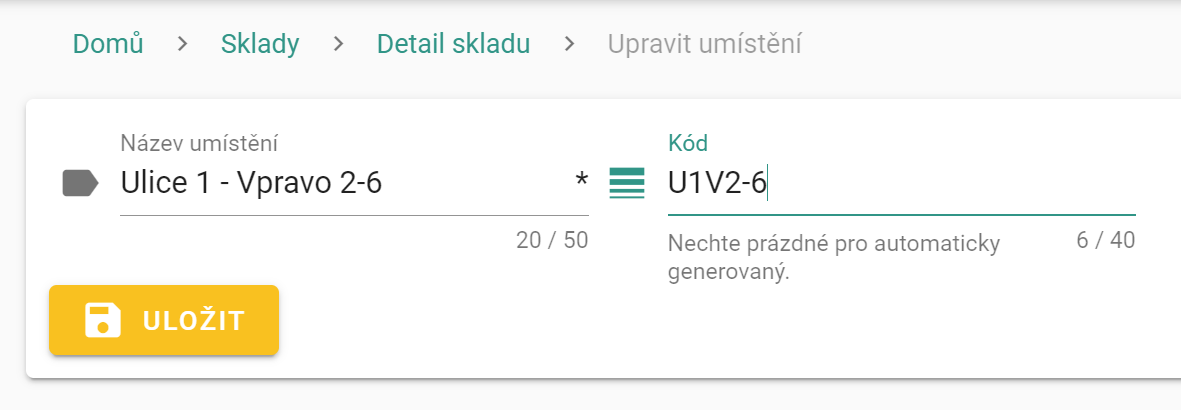
\includegraphics[width=\textwidth]{../png/app/form_stock_location.png}
\caption{Formulář vykreslený pomocí jednotné formulářové komponenty} \label{picture:form-stock-location}
\end{figure}

%%%%%%%%%%%%%%%%%%%%%%%%%%%%%%%%%%%%%%%%%%%%%%%%%%%%%%%%%%%%%%%%%%%%%%%%%%%%%%%%
%%%%%%%%%%%%%%%%%%%%%%%%%%%%%%%%%%%%%%%%%%%%%%%%%%%%%%%%%%%%%%%%%%%%%%%%%%%%%%%%
%%%%%%%%%%%%%%%%%%%%%%%%%%%%%%%%%%%%%%%%%%%%%%%%%%%%%%%%%%%%%%%%%%%%%%%%%%%%%%%%
%%%%%%%%%%%%%%%%%%%%%%%%%%%%%%%%%%%%%%%%%%%%%%%%%%%%%%%%%%%%%%%%%%%%%%%%%%%%%%%%

\section{Realizace podpory pro undo}\label{implementation:undo}

Jak jsme s Pavlem rozhodli v návrhové části (sekce \ref{draft:undo}), undo je realizováno přímou podporou u vybraných akcí.\\
Pro demonstraci celé funkčnosti byla v první fázi vybrána \emph{správa výrobců zboží}, u které je možné procházet kompletní historii změn, a tedy i provádět undo. Základní implementace rozšiřuje běžné \emph{snack messages} přidáním tlačítka \uv{vrátit} (obrázek \ref{picture:undo}). Takovýto toast message má nastavenou zvýšenou či neomezenou životnost, nezmizí tedy během pár sekund, jako ty ostatní. Po využití funkce vrácení se po úspěšném dokončení zobrazí buďto obrázek \ref{picture:undo-after}, či případně chybová hláška.

\begin{figure}[]
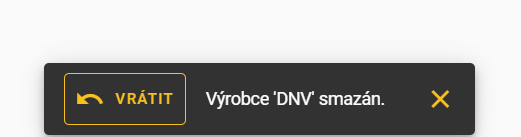
\includegraphics[width=0.6\textwidth]{../png/app/undo_snack.png}
\caption{Undo: Možnost vrácení provedených změn} \label{picture:undo}
\end{figure}

\begin{figure}[]

\includegraphics[width=0.6\textwidth]{../png/app/undo_snack_after.png}
\caption{Undo: Potvrzení vrácení provedených změn} \label{picture:undo-after}
\end{figure}

%%%%%%%%%%%%%%%%%%%%%%%%%%%%%%%%%%%%%%%%%%%%%%%%%%%%%%%%%%%%%%%%%%%%%%%%%%%%%%%%
%%%%%%%%%%%%%%%%%%%%%%%%%%%%%%%%%%%%%%%%%%%%%%%%%%%%%%%%%%%%%%%%%%%%%%%%%%%%%%%%
%%%%%%%%%%%%%%%%%%%%%%%%%%%%%%%%%%%%%%%%%%%%%%%%%%%%%%%%%%%%%%%%%%%%%%%%%%%%%%%%
%%%%%%%%%%%%%%%%%%%%%%%%%%%%%%%%%%%%%%%%%%%%%%%%%%%%%%%%%%%%%%%%%%%%%%%%%%%%%%%%

\section{Generování kódu ze specifikace OpenDoc}\label{implementation:codegen}

Ještě předtím, než jsem začal pracovat na realizaci samotných funkčnostech aplikace, jsem si připravil rozhraní, přes které budu komunikovat s API.\\
Při psaní tohoto kódu jsem se snažil co nejvíce omezit opakování kódu, a tak jsem vymyslel i několik funkcí, které kód podstatně zkracují, ale jak jsem zjistil později, tak do něj zanáší neočekávané chování.\\
Uvedu příklad na funkci pro vytvoření nového odběratele, jejíž hlavička vypadá následovně:\\
\code{create(name, ico, dic, phone, email, website, billing\_address, ...}\\
Uvnitř těla této funkce potřebuji odeslat na API objekt, který vypadá následovně:\\
\code{\{name: <hodnota\_argumentu\_name>, ico: ...\}}\\
Na jeho vytvoření samozřejmě existuje jednoduchá cesta: vytvořit objekt postupně ručně, jeden argument po druhém. To je ale zbytečná ruční práce, do které se navíc jednoduše zanese chyba.\\
Další možností je vše vytvořit v cyklu, který bude iterovat přes všechny názvy atributů - jenže to znamená že buďto musím znovu udržovat seznam těchto atributů, a nebo využít seznam, který už vlastně \emph{mám vytvořený v deklaraci funkce}.\\

\paragraph{Parsování názvů argumentů funkce.} V Javascriptu není plnohodnotná Reflexe, jak ji známe například z Javy, neboť JS je jazyk \emph{prototypový}. Z toho důvodu není tak snadné vytáhnout si v runtime názvy argumentů funkce. Nejbližší nástroj, který se k tomuto přibližuje, je možné vypsat si textový zápis definice funkce, a z jeho hlavičky argumenty vyparsovat - viz ukázka kódu \ref{code:fnArgParse}, která vychází z kódu Christophera Hermanna \cite{fn-parse}.

\begin{listing}[h]
\begin{minted}[linenos,frame=lines]{js}
function getFnArgNames(fn) {
    return fn.toString()
        .match(/[^(]*\(([^)]*)\)/)[1]
        .split(',')
        .map(element => element.split('=')[0].trim())
        .filter(element => !(element === '' 
            || element === null 
            || typeof element === 'undefined')
        );
}
\end{minted}
\caption{Parsování názvů argumentů funkce} \label{code:fnArgParse}
\end{listing}

Jak se ale ukázalo později, toto parsování není použitelné v režimu, kdy je aplikace zkompilovaná pro produkční použití, neboť takový kód je minifikovaný a tudíž neobsahuje celé názvy argumentů funkce, ale pouze jeden znak - výsledný objekt odesílaný na API tedy vůbec neodpovídá specifikaci, a požadavek logicky selže.

\paragraph{Modely datových typů.} Metody parsování argumentů funkce by vůbec nebyly potřeba, kdybych používal standardní modely objektů - tedy před-připravené struktury - které budou mít potřebné klíče v objektech definované. Tím jsem se ale otočil do kruhu, že nechci nic opisovat a duplikovat. V tu chvíli se ale objevila myšlenka, že když mám od kolegy Pavla připravené krásně zdokumentované API, že bych mohl modely automaticky generovat přímo z něj.

\paragraph{Generování modelů datových typů.} Dokumetnaci API, kterou mám dostupnou, je zpracovaná ve standardu OpenAPI 3.0 \cite{openapi-spec}, je tedy možné ji zpracovávat automatizovaně různými nástroji, které stručně popíšu:

\begin{itemize}
    \item \emph{swagger-codegen} \cite{swagger-codegen} Jedná se o velmi robustní nástroj, který dokáže generovat nejen modely, ale také umí vygenerovat kompletní třídy pro komunikace s API. Jeho detaily rozeberu níže.
    \item \emph{swagger-js-codegen} \cite{swagger-js-codegen} Tato knihovna třetí strany má podobné možnosti jako \emph{swagger-codegen}, avšak v době psaní této práce není aktualizovaná pro OpenApi specifikace třetí verze, tudíž pro mé potřeby nevhodná.
    \item \emph{swagger-js} \cite{swagger-js} Doplňující nástroj k \emph{swagger-codegen}, který umožňuje veškeré činnosti provádět přímo za běhu programu pomocí Javascriptu. Pomocí jednoduchého zápisu je například možné i metody spouštět a testovat, avšak pro mé potřeby \emph{generování modelů} je použití taktéž nevhodné.
    \item \emph{OpenAPI Generator} \cite{openapi-generator} Na rozdíl od předchozích - víceméně samostatných - nástrojů se v tomto případě jedná o plugin do WebStorm. Interně používá první zmiňovaný - \emph{swagger-codegen}, takže jejich možnosti popíšu společně na dalších řádcích.
\end{itemize}

Ze čtyř nástrojů zbyly dva padnoucí v úvahu, jeden z nich ale interně používá ten druhý, takže jejich výstupy jsou shodné.\\
Vyzkoušel jsem tedy generátor spouštět s různými parametry, avšak výsledný kód byl na můj vkus vždy zbytečně dlouhý a nezapadal do zbytku codestyle mé aplikace. Zde je nutno poznamenat, že kdybych s tímto generátorem začal, tak ho pravděpodobně použiji i včetně možnosti vygenerovat prakticky celou vrstvu, která realizuje integraci Javascriptu s API - neboť generovaný kód rozhodně není nekvalitní, je velmi robustní a ušetří spoustu času. Protože ale již mám napsanou vlastní vrstvu, která se o API stará, a zakomponovat do ní pouze část generovaného kódu je poměrně složité, a nechci ani vlastní vrstvu zahodit (řeší totiž i některé další věci, které z generátoru nevypadnou - jako například překlady, automatické zpracování chybových stavů nebo zobrazování loaderu), rozhodl jsem se nakonec tento generátor nevyužít. Budu-li ale někdy pracovat na dalším projektu, ke kterému bude dostupná dokumentace ve specifikaci OpenAPI, rozhodně tento generátor zkusím použít hned na začátku implementace.

\paragraph{Vyřešení modelových tříd pomocí formulářových modelů.} Když jsem se rozhodl nepoužívat nakonec generátor kódu z dokumentace API, musel jsem stále ještě vyřešit problém s tím, že má funkce \code{getFnArgNames} nefunguje v produkčním režimu. Řešení nakonec bylo snadnější, než se zdálo, neboť už vlastně mám připravené vlastní modely pro všechny formuláře, jak jsem popisoval v sekci \ref{implementation:formRender} - jedná se o například o konstantu \code{stockLocationForm} z ukázky kódu \ref{code:formfields:def}. Někdo by mohl namítat, že tento model nemá řádně definované typy a další náležitosti, a má zcela pravdu. Ovšem pro základní potřebu \emph{neopisovat ve funkcích zařizujících komunikaci s API} všechny atributy je to více než dostačující - ve funkcích jsem přestal řešit, jaké všechny parametry se do nich dají poslat, a přijímám jednoduše objekt \code{data} - jehož obsahem je právě například \code{stockLocationForm}. Data, která uživatel zadá do formuláře jsou tedy \emph{na přímo, bez jakéhokoliv kopírování} ve stejné formě (samozřejmě po vyřešení serializace, kódování pro URL či převod času do formátu ISO-8601) i odesílána na API - čímž získáváme i zanedbatelné zvýšení efektivity, byť na úkor bezpečnosti (protože nehlídáme typovost obsahu dat), takže to zase taková výhoda není.\\
Samozřejmě se najde i několik metod, do kterých nelze poslat takto přímo definici formuláře, protože se jedná například o pokyn k přesunu zboží mezi umístěním atp. - které se generuje z napípávání zboží, nikoliv z vyplněného formuláře. V těchto několika případech jsem ručně vypsal přiřazení (kterému jsem se snažil z počátku za každou cenu vyhnout), avšak nikdy se nejedná o více než 3 atributy, takže přehlednost by neměla trpět.
Do budoucna budu ještě zvažovat zavedení větší typovosti argumentu \code{data}, který často do API metod posílám, rád bych k tomu využil například JSdoc.

%%%%%%%%%%%%%%%%%%%%%%%%%%%%%%%%%%%%%%%%%%%%%%%%%%%%%%%%%%%%%%%%%%%%%%%%%%%%%%%%
%%%%%%%%%%%%%%%%%%%%%%%%%%%%%%%%%%%%%%%%%%%%%%%%%%%%%%%%%%%%%%%%%%%%%%%%%%%%%%%%
%%%%%%%%%%%%%%%%%%%%%%%%%%%%%%%%%%%%%%%%%%%%%%%%%%%%%%%%%%%%%%%%%%%%%%%%%%%%%%%%
%%%%%%%%%%%%%%%%%%%%%%%%%%%%%%%%%%%%%%%%%%%%%%%%%%%%%%%%%%%%%%%%%%%%%%%%%%%%%%%%

\section{Barevná paleta aplikace}\label{implementation:colors:idempotent}

Barvy použité v aplikaci mají velký vliv na to, jak ji budou její uživatelé vnímat. Když jsem začal s implementací, zvolil jsem pouze pár základních barev, protože v tu chvíli jsem potřeboval funkční kostru aplikace. Postupem času jsem ale začal více přemýšlet o volbě barevné palety a jak ji rozumně zvolit.

\paragraph{Kontrast barvy textu a barvy pozadí.} Základem pro čitelnost textu je správný kontrast barvy textu a barvy pozadí, na kterém se text nachází. Například klasický černý (\#000000) text na bílém (\#FFFFFF) pozadí má kontrastní poměr 21:1, což je nejvyšší možný. Konsorcium W3 vydalo dokument \cite{w3-access-guide}, který popisuje, jak by měl vypadat správně dostupný web - jedna sekce popisuje právě i kontrast. Uvedu úryvek z dokumentu:
\begin{itemize}
    \item \emph{Kontrast (minimum)}: Vizuální prezentace musí mít minimální kontrastní poměr 4,5:1, s následujícími výjimkami:
    \begin{itemize}
        \item \emph{Velký text}: Musí mít kontrastní poměr minimálně 3:1.
        \item \emph{Dekorativní, skryté a doprovodné prvky a logotypy}: Bez požadavků na minimální kontrastní poměr
    \end{itemize}
    \item \emph{Kontrast (pokročilý)}: Vizuální prezentace by měla mít minimální kontrastní poměr 7:1, s následujícími výjimkami:
    \begin{itemize}
        \item \emph{Velký text}: Měl by mít kontrastní poměr minimálně 4,5:1.
        \item \emph{Dekorativní, skryté a doprovodné prvky a logotypy}: Bez požadavků na minimální kontrastní poměr
    \end{itemize}
\end{itemize}

Zde samozřejmě platí, že čím více chceme text na stránce zdůraznit, tím větší kontrastní poměr mu dáme.

\paragraph{Volba barev akčních a informačních prvků.} U informačních prvků je zde poměrně klasické rozdělení: zelená jako potvrzovací, modrá - informativní, žlutá - varovná a červená - chybová. Pro akční tlačítka pak typicky zelená - vytvoření, modrá - zobrazení, žlutá - úprava a červená - smazání. V aplikaci ale většinou nechceme mít tolik barev, moderní aplikace mají čistší, jednudušší design, který když je proveden správně, může snížit zátěž uživatele tolik barvami a zvýšit přehlednost. Velmi často se dnes objevují definice barev jako \code{primary}, \code{secondary} (občas i \code{tertiary}) a \code{accent}, které se jednou zvolí a poté se napříč aplikací používají vlastně jako proměnné.

Výběrem těchto tří barev se zabývá mnoho článků a stránek, teorie, na které ale všichni staví, je pořád stejná: Když volíme tři barvy, existují tři nejčastěji používaná barevná rozložení \cite{color-scheme-pick}:

\begin{enumerate}
    \item \emph{Trojúhelníková}: Rovnoměřné rozdělení barev přes celé barevné schema. Jedná se o velmi výrazné schema, a to i v případě použití nižší barevné saturace. Ideální použití je jedna základní barva a dvě akcentní.
    \begin{figure}[H]
        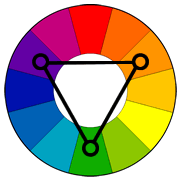
\includegraphics[width=0.2\textwidth]{../png/colors/Triad.png}
        \caption{Barevná paleta aplikace: Trojúhelníkové schema} \label{picture:colors:analog}
    \end{figure}
    \item \emph{Rozděleně-doplňková}: Toto schema vychází z doplňku dvou barev, tedy barev, které jsou v paletě naproti sobě, protější barva je ale rozdělena na dvě. Oproti trojúhelníkovému schematu je méně výrazné, díky čemuž je jednodušší barvy zvolit tak, aby nebyly pro uživatele příliš útočné. Ideální použití je opět jedna základní barva a dvě akcentní.
    \begin{figure}[H]
        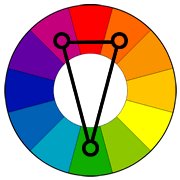
\includegraphics[width=0.2\textwidth]{../png/colors/SplitComplementary.png}
        \caption{Barevná paleta aplikace: Rozděleně-doplňkové schema} \label{picture:colors:splitCom}
    \end{figure}
    \item \emph{Analogová}: Zvolené barvy jsou v barevné paletě přímí sousedé a jedná se tak o \uv{klidné} rozložení, které vytváří jemný design jež je často vidět i v přírodě. Problémem zde může být vhodná volba kontrastu, protože barvy nejsou sami vůči sobě příloš kontrastní a je nutné je od sebe alespoň trochu rozlišit. Ideální použití je jedna dominující barva, druhá doplňková a třetí jako akcentní.
    \begin{figure}[H]
        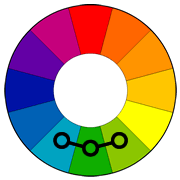
\includegraphics[width=0.2\textwidth]{../png/colors/Analogous.png}
        \caption{Barevná paleta aplikace: Analogové schema} \label{picture:colors:triad}
    \end{figure}
\end{enumerate}

\paragraph{Volba barev pro mou aplikaci.} Jelikož cílem aplikace je pomáhat při práci ve skladu a upozorňovat na důležité zprávy, vyloučil jsem hned ze začátku \emph{analogové} barevné schema, protože jeho barevné rozložení patří spíše na stránky, které jsou pasivnější, nevyžadují tolik interakce s uživatelem a spíše obsah prezentují, než aby vyžadovali jeho zadávání. Zbyly mi tedy velmi podobná rozložení \emph{trojúhelníkové} a \emph{rozděleně-doplňkové}. Podle osobního pocitu jsem vybral základní klidnou barvu: šedozelenou \#009688, a k ní doplňkově-akcentní růžovou \#E91A63 a čistě akcentní tmavě žlutou \#FFC107, jejichž rozložení na barevné paletě je vidět na obrázku \ref{picture:colors:app}. Společně tyto barvy tvoří něco mezi dvěma zvolenými schematy - trojůhelník není ani pravidelný, ani se neblíží k doplňku.\\
\begin{figure}[]
    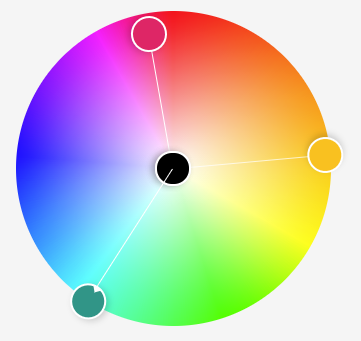
\includegraphics[width=0.4\textwidth]{../png/colors/app.png}
    \caption{Barevná paleta aplikace: Zvolené schema pro mou aplikaci} \label{picture:colors:app}
\end{figure}

\paragraph{Barvy a idempotence akce.} Jelikož mám vybrané dvě akcentní barvy, musel jsem se rohodnout, kde budu kterou z nich používat. Co se týká zobrazování, je vše poměrně jasné: k základní barvě se volně váže doplňkově-akcentní růžová, a čistě akcentní žlutá barva je ponechána pouze pro důležité položky, které je potřeba speciálně zvýraznit. Jiné je to ale u akcí - tlačítek, odkazů apod. Zde jsem se rozhodl barvu tlačítek volit dle idempotence akce, kterou vyvolávají - tedy zda vyvolaná akce způsobuje vedlejší efekty, nebo ji lze vyvolávat stále dokola. Za vedlejší efekty v aplikaci považuji následující situace:
\begin{itemize}
    \item navigace na jinou stránku,
    \item uložení či úprava dat.
\end{itemize}
Naopak akce, které nemají vedlejší efekt jsou všechny ty, které neukládají žádná data ani nemění navigaci, mohou ale měnit aktuální zobrazení stránky, tedy například něco otevřít, skrýt, přesunout, avšak vždy tak, že se jedná o akci pouze na jednom klientu a zůstávají na jedné stránce. Na obrázcích \ref{picture:colors:time_tracker} a \ref{picture:colors:task_fab} je vidět použití jak idempotentních, tak non-idempotentních akcí: tlačítka \emph{storno} a hlavní akční tlačítko pouze skrývají dialog, respektive rozevírají menu, kdežto ostatních tlačítka a volby vždy buďto odesílají data nebo přecházejí na novou stránku.

\begin{figure}[]
    
\includegraphics[width=0.7\textwidth]{../png/app/colors_time_tracker.png}
    \caption{Barvy znázorňující idempotenci akcí: Dialog běžícího času} \label{picture:colors:time_tracker}
\end{figure}
\begin{figure}[]
    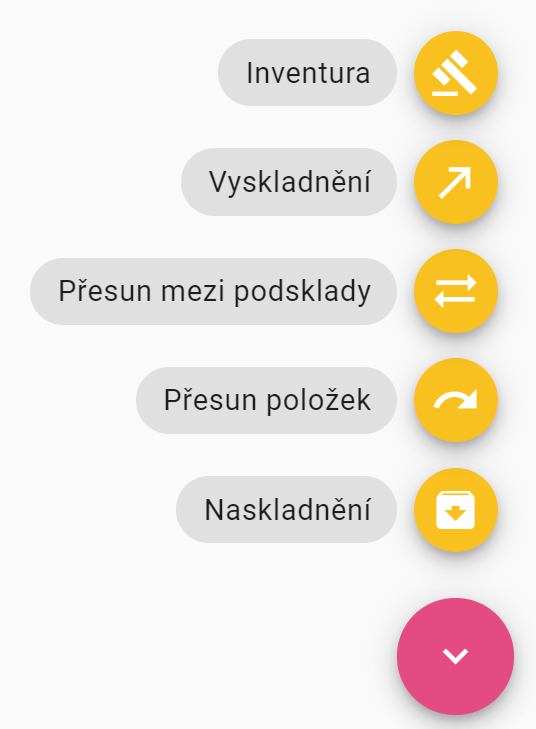
\includegraphics[width=0.3\textwidth]{../png/app/colors_tasks.png}
    \caption{Barvy znázorňující idempotenci akcí: Tlačítko tvorby úkolu} \label{picture:colors:task_fab}
\end{figure}

%%%%%%%%%%%%%%%%%%%%%%%%%%%%%%%%%%%%%%%%%%%%%%%%%%%%%%%%%%%%%%%%%%%%%%%%%%%%%%%%
%%%%%%%%%%%%%%%%%%%%%%%%%%%%%%%%%%%%%%%%%%%%%%%%%%%%%%%%%%%%%%%%%%%%%%%%%%%%%%%%
%%%%%%%%%%%%%%%%%%%%%%%%%%%%%%%%%%%%%%%%%%%%%%%%%%%%%%%%%%%%%%%%%%%%%%%%%%%%%%%%
%%%%%%%%%%%%%%%%%%%%%%%%%%%%%%%%%%%%%%%%%%%%%%%%%%%%%%%%%%%%%%%%%%%%%%%%%%%%%%%%

\section{Záznam stráveného času v úkolech}\label{implementation:time_tracking}

Jedním z požadavků na nový systém byla možnost zaznamenávání stráveného času v úkolech. Jelikož často pracuji v Redmine, což je software pro evidenci požadavků a řízení projektů, kde se čas také zaznamenává, analyzoval jsem, jak se zde se záznamem času pracuje.

\paragraph{Záznam času v Redmine.} V čisté instalaci Redmine je možné čas přidávat k úkolům a nebo celkově k projektům. Zatímco záznam času k projektu se musí provést ze samostatné stránky, záznam času k úkolu je možné spojit s jeho aktualizací. Množství stráveného času ale musí vždy zadat sám uživatel - musí si tedy čas buďto pamatovat, nebo zaznamenávat v další externí aplikaci, či vlastních poznámkách. Jelikož je Redmine open-source, tak existuje hned několik pluginů, které umožňují čas strávený v úkolu stopovat a poté ho zapsat automaticky. Problém, který zde identifikuji já osobně spočívá v tom, že úkolů na Redmine mám často otevřeno i více, nebo naopak žádný, a přesto na některém pracuji například v IDE. Nelze tedy jednoznačně říct, že čas, po který byl úkol otevřen, je stejný jako čas, který byl nad úkolem reálně stráven. Hledal jsem tedy další lepší řešení, a našel vhodnou aplikaci třetí strany.

\paragraph{Záznam času v Toggl.} Toggl je webová aplikace, která nabízí i instalaci nativních agentů pro Windows, Mac a mobilní platofrmy. Díky nainstalovanému agentu je možné spouštět či zastavovat běžící čas klávesovou zkratkou ať už je aktivní browser, IDE, nebo jakýkoliv jiný program. Toto je pro práci, ve které se často přepíná kontext, nebo vznikají pauzy, velmi přínosné. Problém nastává ve chvíli, kdy mám čas uložený v Toggl, ale potřebuji ho zapsat do Redmine. K tomuto účelu jsem napsal vlastní malý doplňěk do Google Chrome, který načte časy uložené v Toggl a otevře záložky s předvyplněnými polemi, ve kterých čas pouze uložím do Redmine. Vše by šlo řešit i zcela automaticky přes API obou služeb, avšak v době psaní tohoto textu ještě není tato synchronizace na dostatečné úrovni a rád mám kontrolu nad tím, které časy vlastně do Redmine zapisuji.

V odstavcích výše jsem se zamyslel nad záznamem času v systému pro řízení obecných projektů. Aplikace pro správu skladu je však přecejen v něčem specifická - jelikož veškerá manipulace se zbožím musí nutně procházet přes ni - všechny položky musí vždy projít čtečkou / být zadány - mělo by být možné stopovat strávený čas přímo v aplikaci

\paragraph{Záznam času v novém skladovém systému.} Pro roli skladníka je poměrně jednoduché automaticky měřit, kolik času strávil v jednotlivých úkolech, a čas odesílat společně s odesláním vyřešení úkolu. U role vedoucího skladu je čas také možné záznamenávat - zde se jedná o přípravu úkolů nebo jejich kontrolou, stále je ale možné práci provádět i mimo tyto obrazovky, například objednávky se mohou zpracovávat mimo systém a pak se pouze jednorázově zadají. Proto jsem také umožnil vedoucímu skladu přidávat strávený čas i ručně.

\paragraph{Pauzování času.} U jakéhokoliv automatického stopování času je nutné mít možnost časomíru pozastavit - typicky například při pauze na oběd či jiné přestávce v práci, během které ale zůstane otevřený jeden úkol. Aplikace vždy zobrazuje, kdy je automatický záznam času spuštěn, a umožňuje ho pozastavit - přičemž u pozastaveného času není možné v úloze provádět žádné akce, až do opětovného spuštění časomíry.

Navrhované řešení automatického záznamu času je samozřejmě možné zcela vypnout v konfiguraci aplikaci, a také ještě bude před ostrým používáním otestováno uživateli. 

%%%%%%%%%%%%%%%%%%%%%%%%%%%%%%%%%%%%%%%%
%%%%%%%%%%%%%%%%%%%%%%%%%%%%%%%%%%%%%%%%

% TODO popsat nový vue.config.js a vue ui - dashboard, deps, analyzet atp.
% 
% TODO JS Flow
% 
% TODO text filtry
% 
% https://itnext.io/yes-this-is-how-to-cache-pages-by-url-with-vue-vue-router-and-keep-alive-component-697ed76896e8
% 
% TODO kontextové menu
% 
% TODO exporty do CSV a JS
% 
% TODO renderer tabulek
% 
% TODO polyfills https://cli.vuejs.org/guide/browser-compatibility.html
% 
% TODO PR do Vuetify?
% 
% TODO funkční specifikace jednotlivých úkolů?

%%%%%%%%%%%%%%%%%%%%%%%%%%%%%%%%%%%%%%%%
%%%%%%%%%%%%%%%%%%%%%%%%%%%%%%%%%%%%%%%%
%%%%%%%%%%%%%%%%%%%%%%%%%%%%%%%%%%%%%%%%
%%%%%%%%%%%%%%%%%%%%%%%%%%%%%%%%%%%%%%%%

\section{Perličky z vývoje}

\subsection{Špatně importované ikony}

Když jsem byl zhruba v polovině tvorby první použitelné verze aplikace, vyšla aktualizace knihovny \emph{Vuetify}, která z verze 1.x poskočila na verzi 2.0. To ssebou neslo poměrně hodně \emph{breaking changes} \cite{vuetify-2-upgrade}, které jsem ale postupně všechny prošel a aplikaci upravil, takže brzy opět fungovala na nové verzi Vuetify.\\
Po nějakém čase jsem si ale všiml, že u checkboxů a dalších formulářových prvků chybí některé jejich součásti - například u checkboxu to bylo hodně výrazné - tam chyběl celý zaškrtávací čtvereček a byl vidět pouze \emph{label}. Nejprve jsem problém ignoroval s tím, že se pravděpodobně jedná o chybu knihovny, a v některé z dalších verzí bude vše opraveno.\\
Když však ale ani po měsíci nebyly checkboxy stále vidět, začal jsem hledat příčinu problému. Samozřejmě jsem nejprve nahlížel do \emph{Nástrojů vývojáře} v prohlížeči, ale tam jsem nic zajímavého nezjistil - pouze to, že z nějakého důvodu se v mé aplikaci narozdíl od oficiální dokumentace Vuetify \cite{vuetify-doc-checkbox} (kde checkboxy samozřejmě fungovaly), nerenderuje kus HTML, který je má na starost. Založil jsem si tedy nový lokální projekt s Vue.js + Vuetify, kde checkboxy samozřejmě také fungovaly. Postupně jsem tedy začal odebírat různé závislosti z npm, abych přišel na to, která knihovna tento problém způsobuje. Při tomto procesu jsem rovnou zauditoval, zda opravdu potřebuji všechny dříve používané závislosti, a upravil i některé kusy kódu tak, aby závislosti již nebyly potřebné, a tedy jsem kód vlastně zefektivnil a zmenšil velikost výsledné aplikace. Stále jsem ale nemohl přijít na to, proč nefungují checkboxy.\\
Teprve asi po 6 hodinách a asi 40x přeinstalovanými všemi závislostmi, jsem se dostal k importu \emph{Material Design Icons} \cite{mdi}. Vuetify ve verzi 2.0 přidalo do možností své konfigurace klíč, který určuje, který ikonový font se má použit. Při migraci na novou verzi jsem použil ukázkové nastavení této hodnoty, tedy \uv{mdi}. V žádném případě mě totiž nenapadlo, že \emph{Material Design Icons (mdi)} a \emph{Material Icons (md)} není to samé!\\
Po chvilce dalšího ladění s importem ikonek vyšlo najevo, že nastavení \uv{mdi} není kompatibilní s načítáním ikon z CDN Googlu, ale musí se použít balíček z npm. V případě, že chcete načítat ikonky z CDN, musí být hodnota \emph{iconfont} nastavena pouze na \uv{md}. Celý problém, na kterém jsem strávil tolik hodin a nechápavých výrazů šel tedy opravit diffem z ukázky kódu \ref{code:mdi:diff}.

\begin{listing}[h]
\begin{minted}[linenos,frame=lines]{js}
-    iconfont: 'mdi',
+    iconfont: 'md',
\end{minted}
\caption{Diff nastavení fontu ikonek ve Vuetify} \label{code:mdi:diff}
\end{listing}

\chapter{Testování}\label{testing}

\section{První testování - během vývoje s odbornou osobou}

První uživatelské testování výsledné aplikace proběhelo při jejím vývoji - 19. 9. 2019 - v době testu byly připravené základní možnost vkládání a úprav většiny entit v systému (skladové položky, dodavatelé atp.) a necelé čtyři ze stěženích úloh - příjem dodávky, naskladnění, inventura a část přesunu zboží.\\
Aplikaci testovala osoba, která mimo jiné činnosti pracuje také se starým skladovým systémem Sysel v roli vedoucího skladu.\\
Testování proběhlo při neformálním setkání v běžné kanceláři, testera jsem instruoval k tomu, aby použil svůj notebook pro zobrazení režimu správce skladu, a mobilní telefon pro roli skladníka. Zatímco na počítači bylo vše v pořádku, neboť byl použit Google Chrome, ve kterém aplikaci spouštím i při vývoji, na mobilním zařízení nejprve nastal malý problém, a to z důvodu použití prohlížeče \emph{Samsung Internet}, který nepodporuje některé moderní Javascriptové konstrukce, na které aplikace spoléhá. Ačkoliv toto nebude pro samotné použití aplikace problém, protože cílové zařízení pro skladníky je jasně dané a aplikace se tam bude otvírat ve WebView, i přesto není na škodu zachovat kompatibilitu i s jinými mobilními prohlížeči, třeba i pro potřeby vedoucích, aby taktéž mohli pracovat z mobilních zařízení. Již před testováním jsem věděl, že je potřeba zavést nějakou detekci prohlížečů a případně uživatele informovat o nekompatibilitě aplikace se zvoleným browserem, ale po této skutečnost jsem ještě zvýšil této úpravě prioritu.\\
Výstupem z tohoto testování vývojové verze aplikace je seznam postřehů, chyb a návrhů na zlepšení, které jsou k nalezení v příloze \ref{ap:testing_notes}.\\
Zde je vhodné poznamenat, že zhruba pětinu všech požadavků a chyb jsem již nějakým způsobem evidoval i před testováním - buďto formou \emph{\uv{TODO} komentářů} přímo v kódu aplikace, nebo kartami v Trellu, avšak pro kompletnost zápisu jsem je ponechal i tam.

%%%%%%%%%%%%%%%%%%%%%%%%%%%%%%%%%%%%%%%%%%%%%%%%%%%%%%%%%%%%%%%%%%%%%%%%%%%%%%%%
%%%%%%%%%%%%%%%%%%%%%%%%%%%%%%%%%%%%%%%%%%%%%%%%%%%%%%%%%%%%%%%%%%%%%%%%%%%%%%%%
%%%%%%%%%%%%%%%%%%%%%%%%%%%%%%%%%%%%%%%%%%%%%%%%%%%%%%%%%%%%%%%%%%%%%%%%%%%%%%%%
%%%%%%%%%%%%%%%%%%%%%%%%%%%%%%%%%%%%%%%%%%%%%%%%%%%%%%%%%%%%%%%%%%%%%%%%%%%%%%%%

\section{Druhé testování - alfa verze kompletní aplikace}

Dne 6. 12. 2019 proběhlo druhé uživatelské rozhraní, které bylo od prvního testování mnohem obsáhlejší. Vydal jsem se do dvou skladů menších rozměrů, ve kterých jsem otestoval celkem čtyři osoby zde pracující.\\
Průběh testování probíhal s každou testovanou osobou stejně, podle následujícího rozpisu:
\begin{enumerate}
	\item Pokud byl ve skladu používán již nějaký skladový systém, pozoroval jsem chvíli, jak se s ním pracuje a jaké jsou nejdůležitější úkony.
	\item Položil jsem testované osobě několik otázek dle \emph{Dotazníku před testováním} (viz příloha \ref{ap:testing_questions}).
	\item Provedli jsme samotné testování aplikace, dle připravených úkolů (viz příloha \ref{ap:testing_tasks}).
	\item Položil jsem testované osobě několik dalších otázek, dle \emph{Dotazníku po testování} (viz příloha) \ref{ap:testing_questions}).
	\item Jako poděkování jsem nabídl vánoční perníčky vlastní spolutvorby.
\end{enumerate}

V tomto textu budu vypisovat pouze nejdůležitější odpovědi a poznatky z testování, zápis požadavků a problémů zpracovaný do strukturovaného seznamu je dostupný v příloze \ref{ap:testing_requirements}. Také nebudu zmiňovat celá jména testovaných osob, neboť to pro výstup testu není podstatné.
\\
Během samotného testování aplikace jsme používali reální zařízení Zebra TC-25, na kterém jsem měl předinstalovanou aplikaci s podporou čtečky čárových kódů. Také jsem měl vytištěno několik čárových kódů, kterými se identifikují výrobky a dále několik kódů pro výrobky samotné. Kromě Zebry - na které jsem testoval především roli \emph{skladníka}, jsme vždy využili i notebook, který je běžně ve skladu používán - na tom se naopak testovala role \emph{vedoucího skladu}.

%%%%%%%%%%%%%%%%%%%%%%%%%%%%%%%%%%%%%%%%%%%%%%%%%%%%%%%%%%%%%%%%%%%%%%%%%%%%%%%%
%%%%%%%%%%%%%%%%%%%%%%%%%%%%%%%%%%%%%%%%%%%%%%%%%%%%%%%%%%%%%%%%%%%%%%%%%%%%%%%%

\subsection{Testování v prvním skladu}

Nejprve jsem začal ve skladu e-shopu, jehož sortimentem je převážně obuv, přípravky pro péči o tělo a zdraví, výbava domácnosti a také elektronika. Sklad se nachází v samostatné místnosti v průmyslové budově, a obsahuje odhadem kolem čtyř set umístění, přičemž \uv{umístění} je krabice polepená štítkem, kterých je na sobě mezi čtyřmi až šesti, a jsou vyskládány v řadách.\\
V tomto skladu je aktuálně používán skladový systém Sysel, ze kterého vycházela i analýza požadavků pro nově tvořený systém, takže se nabízela možnost přímého srovnání obou systémů.\\
Ještě před započetím testování jsem si zavedl do nového systému dvě reálná umístění tohoto skladu a jeden konkrétní výrobek. Bohužel kvůli povaze skladovaného zboží jsem nenašel více stejných skladových položek, a tak jsme nemohli efektivně simulovat práci s více kusy stejné položky.

%%%%%%%%%%%%%%%%%%%%%%%%%%%%%%%%%%%%%%%%%%%%%%%%%%%%%%%%%%%%%%%%%%%%%%%%%%%%%%%%

\subsubsection{Postřehy z testování s první osobou}
\emph{Žena, 42 let, dříve zdravotní sestra, nyní majitelka eshopu.}

\paragraph{Dotazník před testováním.} Z dotazníku provedeného před samotným testováním vyplynulo, že první testovaná osoba od skladového systému nejvíce očekává informace o umístění požadovaného kusu zboží během vyskladňování. Dále jí vyhovují režimy pípání při načítání kódů - krátké pípnutí jako potvrzení a dlouhé jako chyba. Také považuje za důležité mít v systému funkci průchodu historie umístění položky - pro případ, že na deklarovaném umístění se položka ve skutečnosti nenachází. Naopak jako problematické označila například nutnost posouvat se na obrazovce až na konec v případě, že něco naskladňuje, protože nejnovější položka se přidá na konec seznamu. Také jí vadí absence evidence kapacity umístění, kterou si vede v separátním souboru uloženém na notebooku, který je ve skladu.\\

\paragraph{Testování nové aplikace.} Co se týká testování nového systému, přistupovala k němu spíše s rozvahou, často tápala kudy má pokračovat, nebo co má zadávat. Toto bylo částečně způsobeno tím, že na rozdíl od Sysla, je v novém systému prohozeno pořadí napípávání kusu zboží a umístění, ze kterého je sebráno, či na které je uloženo. Největší problémy dělalo hledání přidávání nových věcí - ať už skladových položek nebo úkolů, které je řešeno pluskem ukotveném v pravém dolním rohu obrazovky. Během testování mi bohužel příliš nesdělovala své myšlenky, které by byly přínosné pro případné úpravy, největších problémů jsem si ale všiml i přesto a poznamenal jsem si je.\\
Některé úkony prováděla poprvé, neboť je nedělá ani v současném skladovém systému - jednalo se například o založení nové skladové položky. Po nalezení příslušné akce ale bez problémů vyplnila potřebná pole, bohužel ale nedokázala určit, která pole jsou povinná\footnote{Povinnost polí je ve formulářích označována hvězdičkou, a při chyb jsou pole označena červeně, viz obrázek \ref{picture:test:required_fields}. Toto označení považuji i po tomto testu za dostatečné.}.\\

\begin{figure}[h]

\includegraphics[width=\textwidth]{../png/app_testing/required_fields.png}
\caption[Označení povinných polí formuláře]{Označení povinných polí formuláře: Název je povinný, a uživatel v něm již měl kurzor, nebo se pokusil formulář odeslat. Model je povinný, ale uživatel do něj ještě neklikl. Výrobce je výběr ze seznamu, ale povinný není.} \label{picture:test:required_fields}
\end{figure}

Častokrát jsme také narazili na to, že některé úkony jsou v novém systému složitější, než ve starém - již například zmiňovaná nutnost nejprve napípnout umístění. Starý systém nabízel automatické doplnění umístění, pokud byl napípnut výrobek, který je v systému pouze na jednom místě. Tato funkce ale někdy nebyla stoprocentně spolehlivá, a tak jsem se rozhodl mechanismus předělat tak, aby se vždy nejprve volilo umístění, od čehož jsem si sliboval snížení chybovosti především ve větších skladech. Rozumím ale argumentu, že pro sklad, který víceméně celý spravuje jeden člověk, je toto zbytečné ztížení, avšak již v době psaní této práce je vypsáno nové téma, které bude na tuto práci navazovat, a jehož cílem bude právě optimalizace procesů na malých skladech - považuji tedy za korektní můj současný přístup, a to že v systému lze provést vše, kvalitně, avšak někdy zbytečně zdlouhavě, a efektivnější procesy se mohou dále optimalizovat.

\paragraph{Dotazník po testování.} Po skončení testování jsem se vyptal na několik věcí přímo se týkajících nového systému. Jako největší slabinu označila především menší písmo a pro ni nižší přehlednost, na druhé straně uvítala zobrazování fotografií skladové položky. Nejvíce jí chyběla možnost zadat přímo počet kusů položky, napípávání všech jednotlivých kusů postupně ji nevyhovovalo. Při otázce, zda by ji dávalo smysl namísto pípání, nebo jako doplněk k němu, používat vibrace zařízení, ji to přišlo jako zbytečnost, protože zvukový signál prý vnímá lépe.

%%%%%%%%%%%%%%%%%%%%%%%%%%%%%%%%%%%%%%%%%%%%%%%%%%%%%%%%%%%%%%%%%%%%%%%%%%%%%%%%

\subsubsection{Postřehy z testování s druhou osobou}
\emph{Muž, 40 let, dle svých slov \uv{majitel největšího e-shopu v ČR s mizerným skladovým systémem}\footnote{První část tvrzení není pravda, druhou nemohu objektivně posoudit.}.}

\paragraph{Dotazník před testováním.} Již z dotazníku provedeného před testování bylo zřejmé, že se jedná o člověka, který se se skladovými systémy již setkal, a to i ve větším měřítku než pouze ve skladu eshopu. Co se konkrétně aktuálně používaného systému - tedy Sysla - týká, vyhovuje mu především propojení s eshopem, rychlost a individuální řešení. Na druhé straně si ale stěžuje na některé kostrbaté funkce, jako příklad uvedl, že když přiřadí EAN k nové položce, ale ten stejný EAN už byl dříve použit, tak se ze staré položky odebere, aniž by o tom byl uživatel informován. Od skladového systému očekává především efektivní využití zaměstnanců, jedná-li se o velký sklad, a také snížení chybovosti. Za nejpalčivější procesy současného řešení označil expedici a inventuru.

\paragraph{Testování nové aplikace.} V systému se pohyboval velmi rychle, a většina záseků byla způsobena spíše tím, že si chtěl něco upřesnit, nebo mi k tomu dát zpětnou vazbu. Efektivně využíval našeptávací pole, ve kterých začal vždy psát a klávesou enter potvrzoval zvolené položky, na rozdíl od předchozí testované osoby, která více používala myš. S přidáváním nových věcí pomocí šipky či pluska v pravém dolním rohu problém neměl, pouze na domovské obrazovce, kde se tento prvek používá pro tvorbu nových úkolů, mu přijdou dva kliky zbytečné a radši by měl seznam dostupný přímo, aby úkoly tvořil jen jedním kliknutím. Při naskladňování byl lehce zmatený nutností pípat nejprve umístění, a teprve poté skladové položky, ale rychle se nový postup naučil. Při otázce, jak ze systému zjistí, kde požadovanou položku nalezne, poměrně překvapivě šel hledat do zadání, přestože tato informace se vztahuje ke konkrétní položce. Až když v zadání tuto informaci nenašel, zkusil rozkliknout skladovou položku, kde už požadovaná informace byla. Během testování zanadával pouze jedenkrát, a to ve chvíli, kdy zjistil, že při přesunu položek mezi umístěními musí nejprve všechny položky napípat při jejich zvednutí, a znovu při jejich položení na cílové umístění. Tento proces mi přišel od stolu poměrně logicky, protože pouze tak je možné zaručit, že skladník položí opravdu všechny položky, ale uživatel to vidí jinak - tento konkrétní tester při tomto zjištění aplikaci pojmenoval \uv{skladový systém buzerant}.

\paragraph{Dotazník po testování.} Po testování jsem se jako v prvním případě zeptal na několik dopřesňujících otázek. Na novém systému oceňoval nový a moderní design, přišlo mu ale že většina důležitých informací je vždy orientována až moc do levé horní části stránky. Uvítal novou možnost nastavit jednomu účtu role skladníka i vedoucího současně, u práce se skladovými položkami mu ale chyběla možnost přímo nastavit jejich množství. Co se konfigurovatelnosti domovské obrazovky týká, navrhuje i možnost zobrazovat úkoly ne ve sloupcích, ale v řádcích. Také má zkušenosti se skladováním zboží více různých majitelů, naopak šarže mu blízké nejsou, ale rád by o nich zjistil více, protože jimi označené zboží plánuje do budoucna také skladovat.

%%%%%%%%%%%%%%%%%%%%%%%%%%%%%%%%%%%%%%%%%%%%%%%%%%%%%%%%%%%%%%%%%%%%%%%%%%%%%%%%
%%%%%%%%%%%%%%%%%%%%%%%%%%%%%%%%%%%%%%%%%%%%%%%%%%%%%%%%%%%%%%%%%%%%%%%%%%%%%%%%

\subsection{Testování v druhém skladu}

Po otestování prvních dvou osob jsem se přesunul do druhého skladu, který na rozdíl od toho prvního žádný skladový systém nepoužívá, přestože počet skladovaných produktů také není nejmenší. Osoby pracující v tomto skladu si ale veškerá umístění pamatují, a umístění by zde ani nebylo zcela jednoduché zřídit, neboť se jedná víceméně o chodbu a jednu místnost v přízemí rodinného domu, kde je na první pohled vše uloženo tam, kam se to zrovna vešlo. Jelikož se ale i přesto o zavedení skladového systému do budoucna uvažuje - pravděpodobně již v nových prostorech, kam by se měl sklad přemístit, bylo testování na místě.\\
Kvůli nižším teplotám v samotném skladu jsme testování prováděli v zázemí, u notebooku, a umístění jsme simulovali mými čárovými kódy, které jsem měl předem vytištění. Jako skladové položky jsme poté využili běžné zboží, které bylo dostupné v kuchyni, a od kterého jsme měli k dispozici více než 1 kus.

%%%%%%%%%%%%%%%%%%%%%%%%%%%%%%%%%%%%%%%%%%%%%%%%%%%%%%%%%%%%%%%%%%%%%%%%%%%%%%%%

\subsubsection{Postřehy z testování s třetí osobou}
\emph{Žena, 30 let, živnostnice, administrátorka a správkyně skladu e-shopu.}

\paragraph{Dotazník před testováním.} Zkušenosti se skladovými systémy zde byla nulová, čímž odpadla i většina dalších otázek, které jsem v dotazníku před testováním pokládal. Co se očekávání od takového systému týká, tak by očekávala především časové usnadnění práce ve smyslu zlepšení orientace, případně i poskytování vhodných statistik jako například trendů ve vyskladňování zboží - doporučování k objednání apod. Během této diskuze jsme se dostali až k bodům, které se již týkají spíše systému e-shopu, jako například nabízení slev na produkty, které se dlouhodobě neprodávají, ale přesto jsem si je poznamenal.

\paragraph{Testování nové aplikace.} Během samotného testování projevila poměrně velkou komunikativnost, sdílela své pocity a myšlenkové pochody, což bylo pro účely uživatelského testování naprosto skvělé. Z jejího testování tedy mám nejdelší zápis a nejvíce návrhů na zlepšení, o kterých budu dále přemýšlet. Stejně jako se již objevilo dříve, měla poměrně problém s pluskem v pravém dolním rohu, avšak jakmile jej jednou nalezla, tak již věděla, co v něm očekávat a práce se rapidně zrychlila. Mezi nejzajímavější návrhy ke zlepšení patří možnost zasílat skladníkům přímé notifikace, že jim byl přiřazen nový úkol. Poměrně problematické pro ni bylo pochopit, že nejprve je vždy nutné naskenovat kód umístění a teprve poté kód skladové položky, i když již tento proces procházela poněkolikáté, tak skoro vždy provedla skenování v opačném pořadí, přestože systém poskytuje hlášky, jaké skenování je očekáváno. Z toho tedy vyplynulo, že se hlášky musí ještě zlepšit - prostor pro to je a hned při testování jsem si zapsal návrhy na konkrétní úpravy. Podobný problém se zobrazovanými informacemi na stránce nastal i při vyskladňování, ve kterém ji mátla informace o umístění, na které má vyskladňované zboží přemístit - místo toho si myslela, že na uvedeném umístění najde zboží k vyskladnění. I na tento bod jsem měl již při testování zapsaný návrh na zlepšení.\\
Diskuze proběhla také nad funkcí záznamu stráveného času, u kterého marně hledala funkcionalitu pauzy, kterou jsem hodlal do aplikace tak jako tak přidat. Matoucí ale byl dialog při odchodu z rozpracované úlohy, který se ptá, zda chce uživatel uložit čas - v testerce vyvolal dojem, že když čas uloží nyní, tak už nikdy později nepůjde přidat čas další. 

\paragraph{Dotazník po testování.} // TODO

%%%%%%%%%%%%%%%%%%%%%%%%%%%%%%%%%%%%%%%%%%%%%%%%%%%%%%%%%%%%%%%%%%%%%%%%%%%%%%%%

\subsubsection{Postřehy z testování s čtvrtou osobou}
\emph{Žena, 32 let, živnostnice, majitelka e-shopu.}

\paragraph{Dotazník před testováním.} Jelikož se jedná o stále stejný sklad, ani poslední testovaná nemá zkušenosti se skladovými systémy, a proto je většina otázek ze sekce \uv{před testováním} spíše přeskočena. Od skladového systému očekává, že jí řekne, kde se skladová položka nachází, další nápady jsem z ní ale pro tuto chvíli nedostal.

\paragraph{Testování nové aplikace.} Při testování aplikace se projevila jako inteligentní, ale dosti skeptická k novým věcem, největší problém bylo vždy požadovanou věc v systému nalézt, a po jejím prvním projití již druhý průchod byl velmi rychlý. Z tohoto testování také pochází některé citace, které nešlo do textu nezahrnout:
\begin{itemize}
	\item \emph{Během hledání, kudy se zakládá nová skladová karta:} \uv{Tady nikde není nový produkt... Tohle? Sorry jako ale takovýhle plus? ... Ježiš marja zase dole v pravym rohu!}
	\item \emph{Během vyskladňování typu \uv{expedice}, což vlastně znamená přemístění na jiné místo, kde se bude balit:} \uv{Já si to teda vezmu z U2\footnote{označení umístění} a přemístím to na U3 a to je uplně dementní, na tom strávíme hrozně moc času!}
\end{itemize}
Při dotazu, zda nějak naloží s informací, že daná skladová položka je někdy v krabici, která má vlastní kód, a uvnitř je deset kusů zboží, prohlásila, že namísto aby si vytvořila v systému nový kód této položky, který bude reprezentovat 10 kusů, tu krabici rozbalí a po jedné položky naskladní. Na rozdíl od předchozích testerů neměla žádné problémy s pochopením pořadí pípání umístění a položek, v tomto se zorientovala velmi rychle. U dialogu se záznamem stráveného času namítla poměrně věcný bod, že čas by se mohl ukládat vždy, protože takto by pro skladníka bylo jednodušší s časem manipulovat - načež jsem usoudil, že tuto funkcionalitu budu muset ještě znovu promyslet.

\paragraph{Dotazník po testování.} Při pokládání otázek po testování jsem byl opět svědkem odmítavého přístupu k zavedení podobného systému, a to větou \uv{Já bych to nepoužívala ani náhodou, přijde mi to hrozně zdlouhavý, že bych strávila víc času, než prostě jen vezmu, zabalim, nalepim štítek.}. Systém jako takový ale špatně nedopadl, veškeré potřebné informace zobrazoval, dokonce jí přišlo jako dobrý nápad umožnit i vibrace zařízení jako doplněk k pípání, a stejně tak jí dával smysl spouštění rychlých akcí za pomoci načtení kódu odkudkoliv z aplikace.

%%%%%%%%%%%%%%%%%%%%%%%%%%%%%%%%%%%%%%%%%%%%%%%%%%%%%%%%%%%%%%%%%%%%%%%%%%%%%%%%
%%%%%%%%%%%%%%%%%%%%%%%%%%%%%%%%%%%%%%%%%%%%%%%%%%%%%%%%%%%%%%%%%%%%%%%%%%%%%%%%

\subsection{Shrnutí testování a největší problémy}

Uživatelské testování jako takové považuji za velmi úspěšné. Aplikace byla použitelná, všechny potřebné věci v ní testeři byli schopni nakonec provést, byť v některých případech k tomu vedla trnitá cesta.\\
Při testování se vyskytlo pouze několik aplikačních chyb, které jsme byli schopni obejít a pokračovat v testu, žádná z chyb nebyla zcela kritická.\\

Jelikož nejpalčivější problémy uživatelského rozhraní se často opakovaly u více testerů, popíšu je nyní hromadně:

\paragraph{Tvorba nových věcí pomocí pluska v pravém dolním rohu.} Na obrázku \ref{picture:test:add_before} je vidět detail seznamu skladových položek, odkud jsem po testerech chtěl vložit založit novou skladovou položku. Většina z nich měla problém s nalezením žlutého \uv{plus} v pravém dolním rohu, přes které se nová položka přidává. Při dalším použití tohoto plus již sice vše našli rychle, ale i přesto jsem se rozhodl v reakci na tento problém přidat možnost vkládání položek i na konec tabulky, jak je vidět na obrázku \ref{picture:test:add_after}. Tato volba se zobrazuje pouze na tabletech a větších zařízeních, na mobilních zařízeních je plusko dostatečně v zorném úhlu, a navíc se na zařízeních s Androidem jedná o standardní komponentu, na kterou jsou uživatelé zvyklí.

\begin{figure}[h]
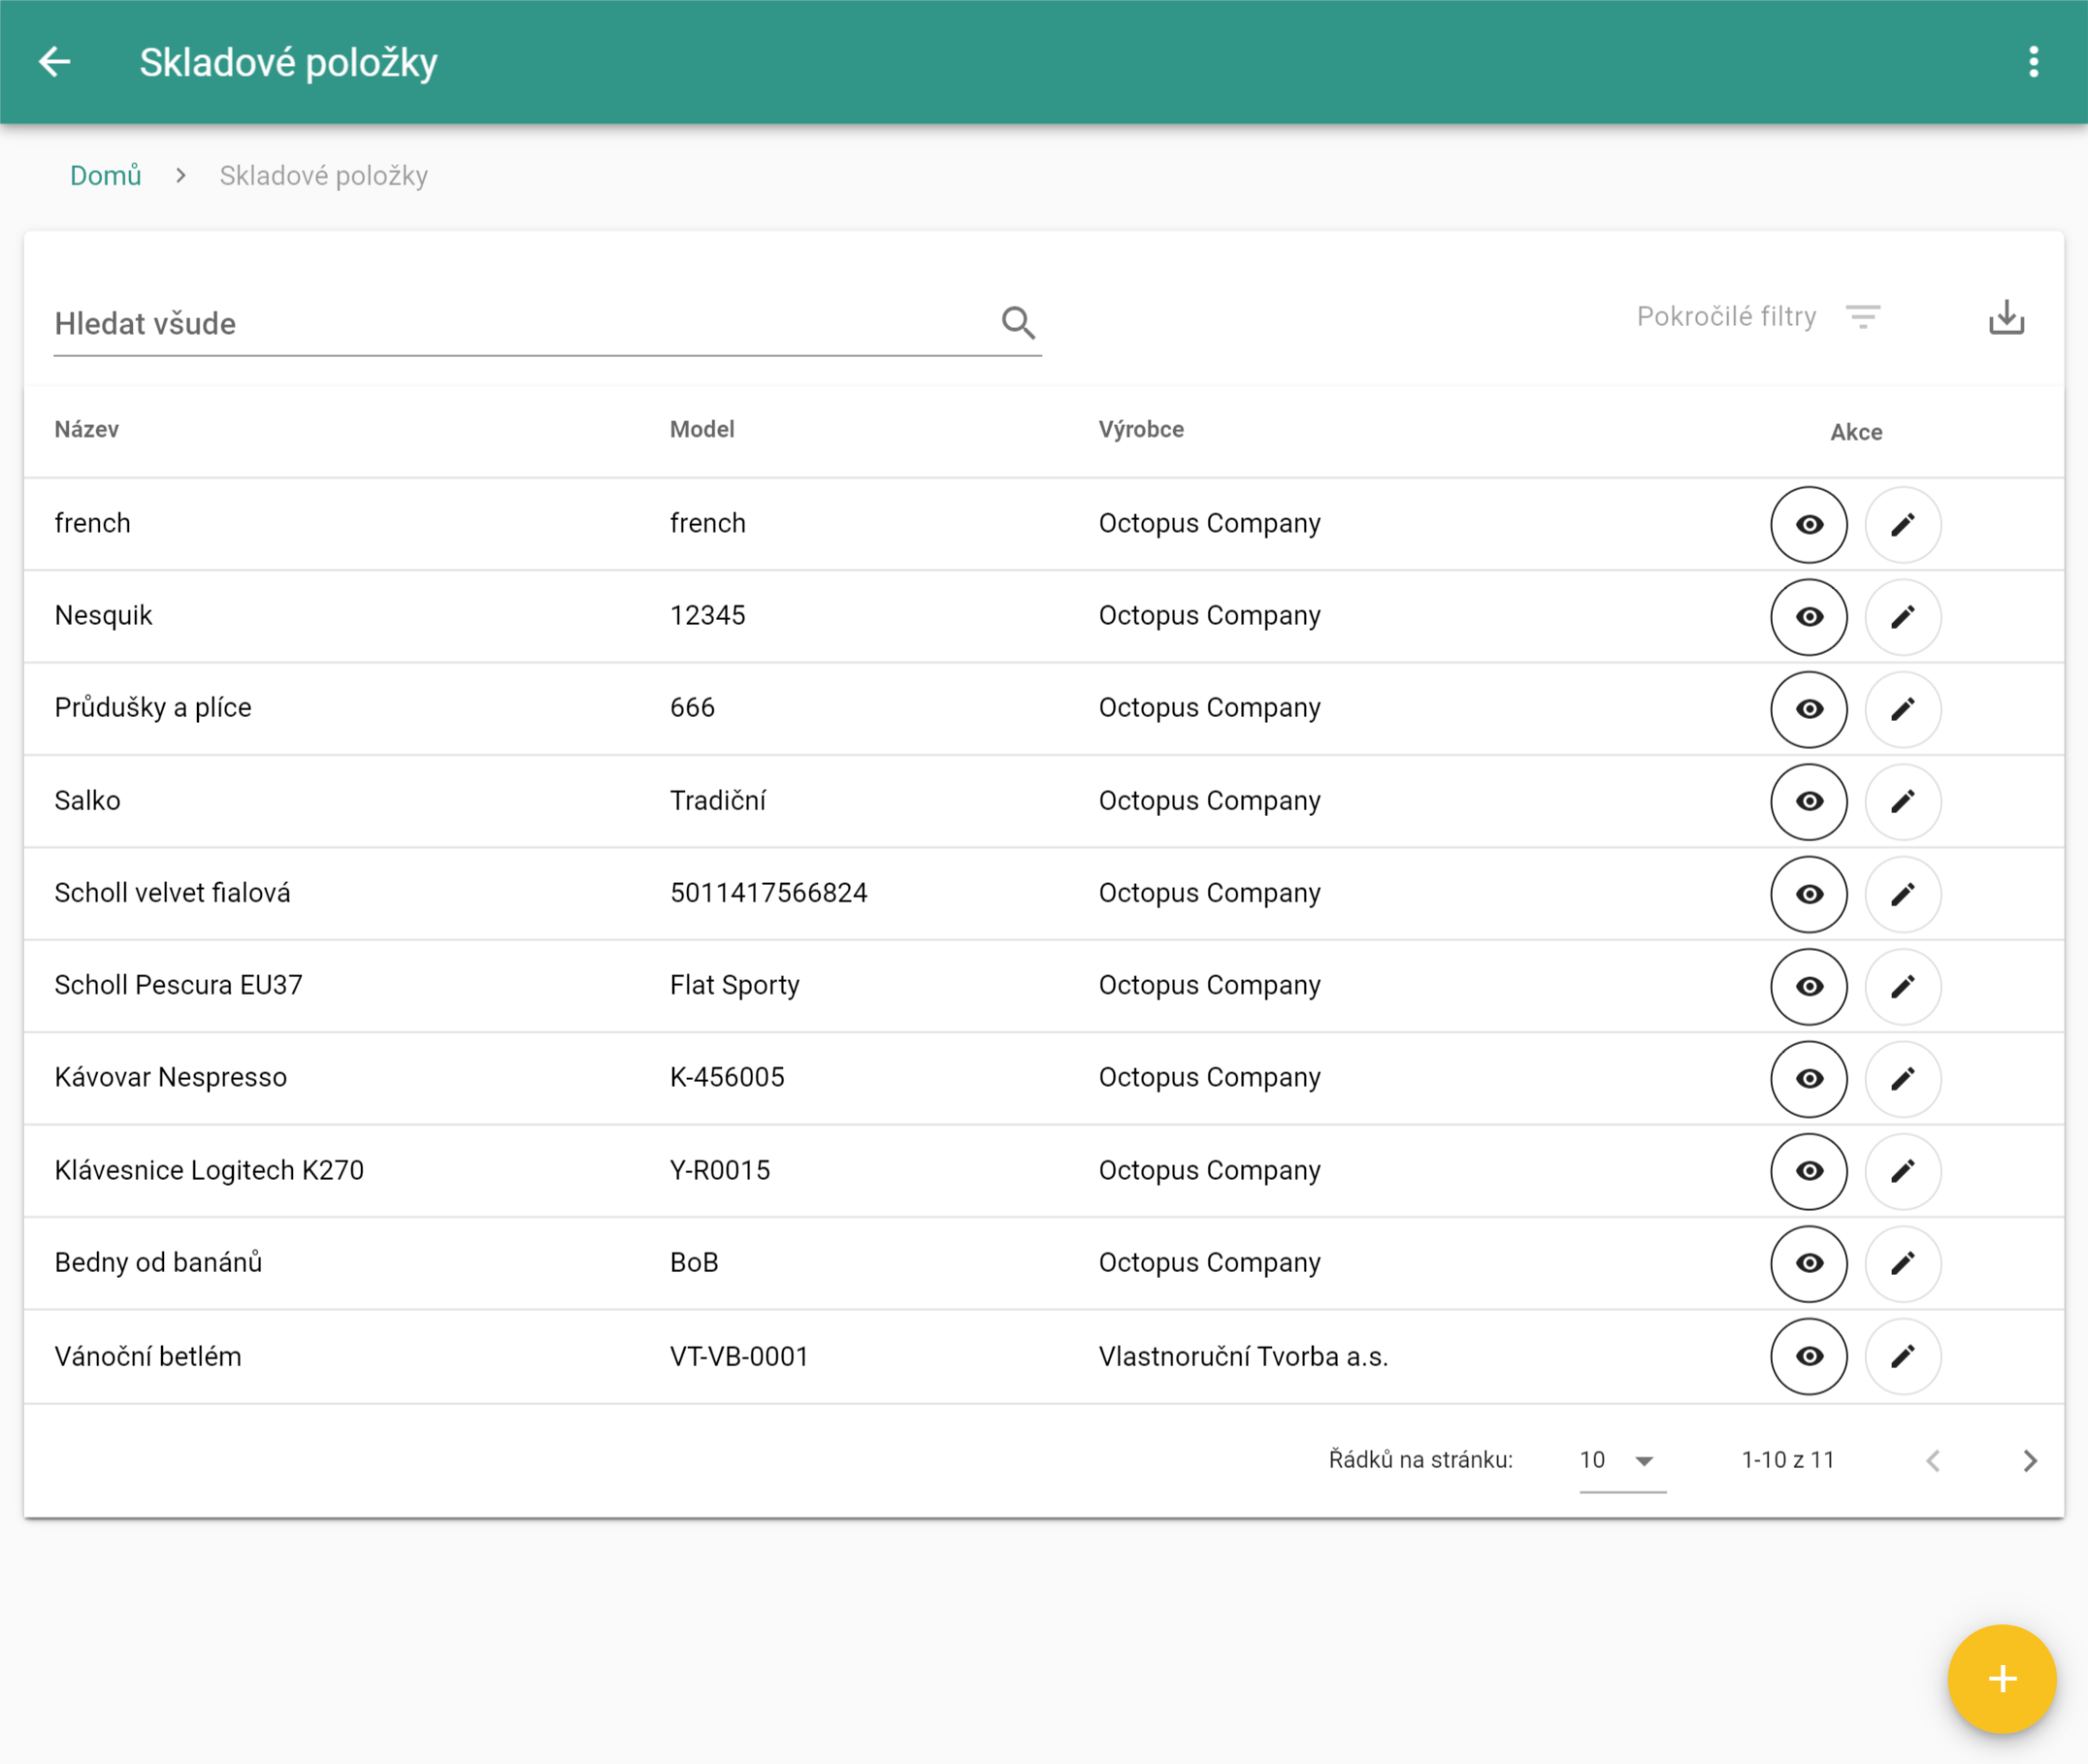
\includegraphics[width=\textwidth]{../png/app_testing/plus_before.png}
\caption{Tvorba nové skladové položky: stav před uživatelským testováním} \label{picture:test:add_before}
\end{figure}

\begin{figure}[h]
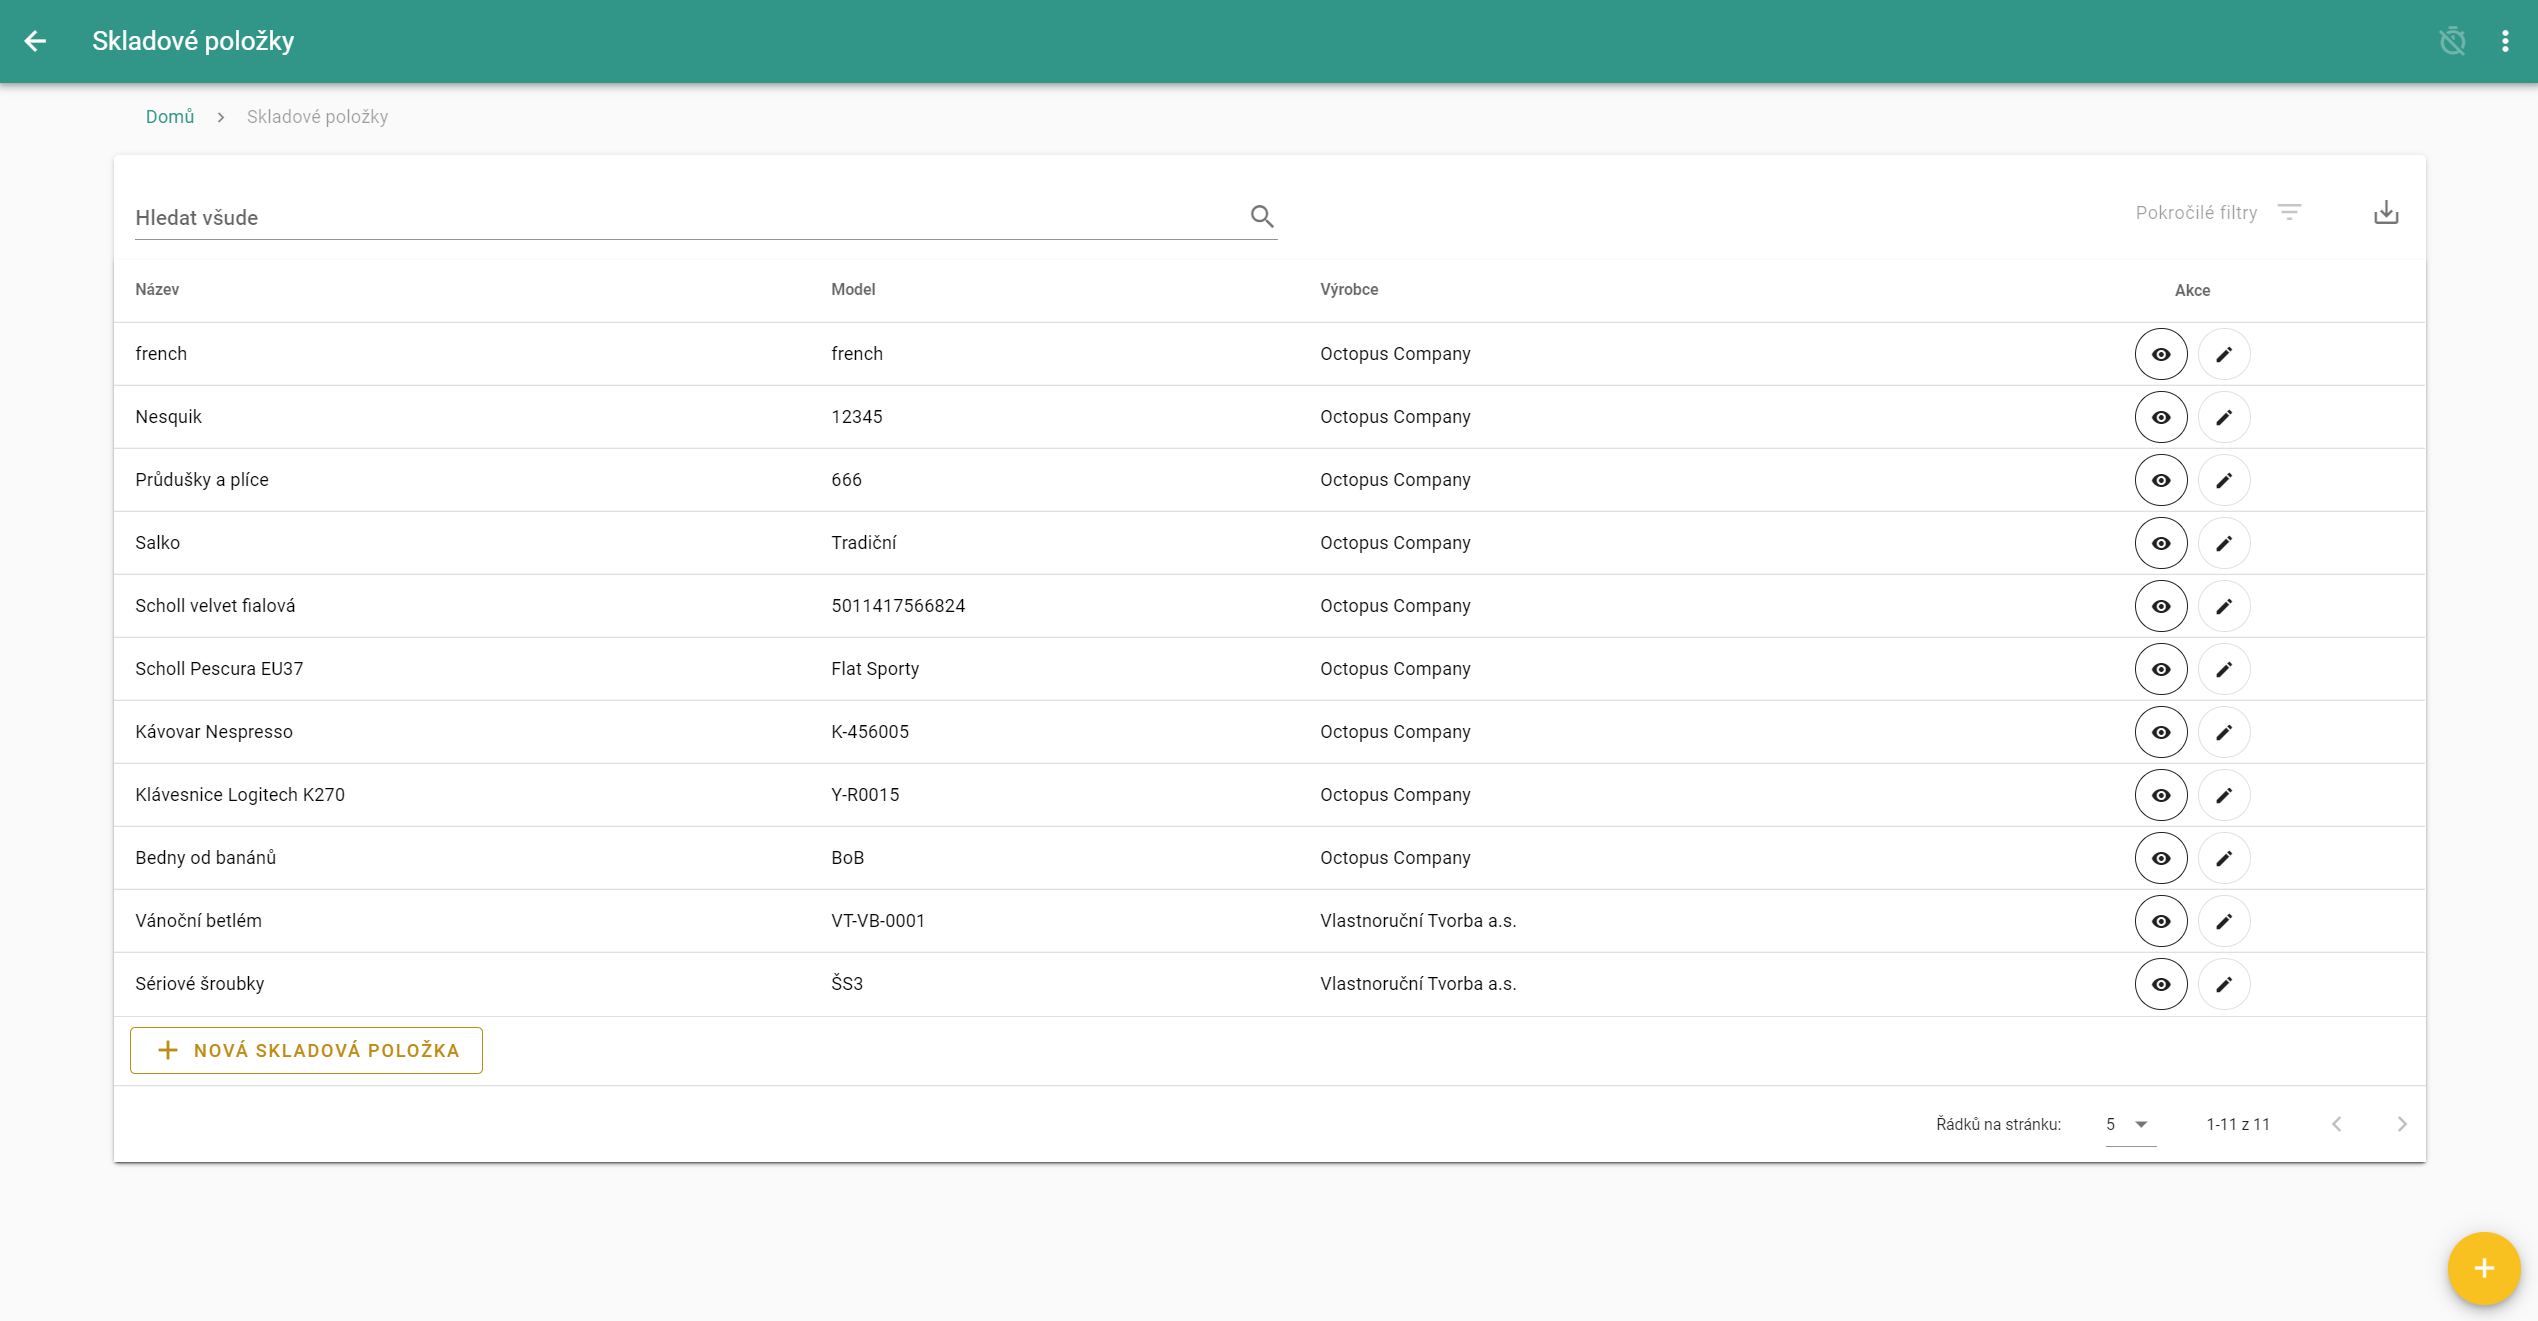
\includegraphics[width=\textwidth]{../png/app_testing/plus_after.png}
\caption{Tvorba nové skladové položky: úprava po testování} \label{picture:test:add_after}
\end{figure}


\paragraph{Přesun mezi umístěními a dvojité pípání položek.} Dalším velmi palčivým problémem, na který si uživatelé stěžovali, byla nutnost znovu zvolit všechny položky, které se chystají přesunout na cílové umístění při přesunu položek, či při vyskladňování typu \uv{expedice}. Při těchto úkolech je potřeba nejprve napípat zboží, které skladník \emph{sbírá}, a poté jej napípat znovu, při \emph{pokládání} na cílové umístění. Při přesunech, které mají pevně dané cílové umístění může být ale druhé pípání velmi otravné, a tak jsem do aplikace přidal \emph{volitelnou} možnost po označení cílového umístění, na něj přesunout vše, co má skladník aktuálně \uv{u sebe}. 
TODO


\paragraph{Ruční nastavení počtu kusů zboží.} Funkce, kterou všichni testeři shodně žádali, je umožnění ruční manipulace s počtem načteného zboží, což umožní jednodušeji zadat větší množství položek, avšak může to také zvýšit chybovost. Přesto jsem se rozhodl nastavení přímé kusovosti uživatelům umožnit, a v případě, že by to nějakému provozovateli skladu vadilo, může být tato komponenta zobrazována na základě nastavení konkrétní instance skladového systému.

// TODO screen?

\paragraph{Zavření detailu skladové položky.} Detaily o skladové položce se během práce na úkolu zobrazují v komponentě nazývané \uv{bottom sheet}, což je vlastně modální okno, které vyjíždí ze spodní části obrazovky a zabírá celou její šířku. Uživatelské testování ukázalo, že uživatelé mají často problém tento pohled zavřít, což se provádí dotykem (či kliknutím) kamkoliv mimo. Po zvážení těchto nejasností jsem se ale rozhodl přidat do jeho pravého horního okraje i tlačítko na jeho zavření, viz obrázek \ref{picture:test:close_bottom_sheet}.

\begin{figure}[h]
\frame{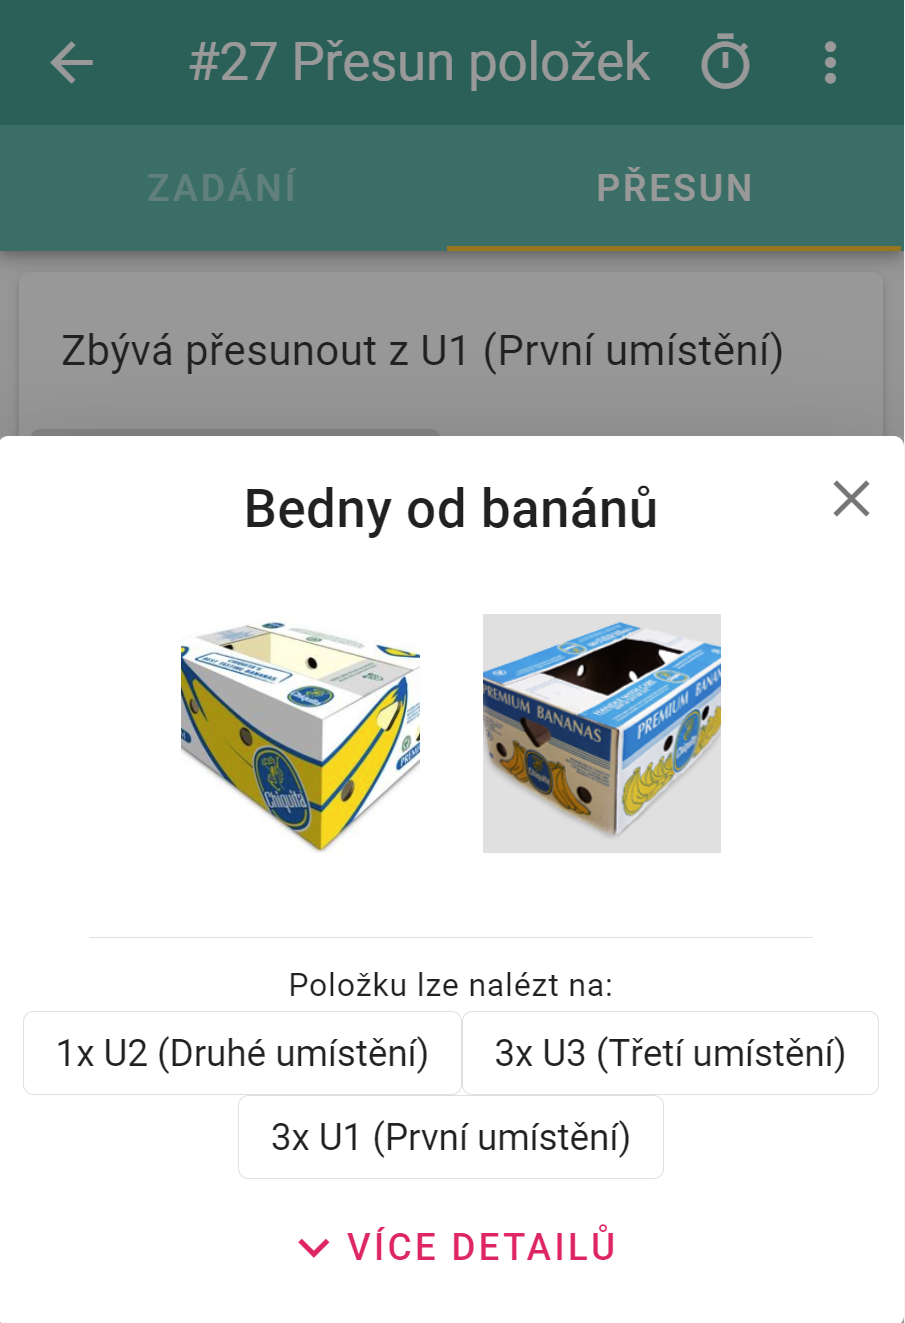
\includegraphics[width=0.4\textwidth]{../png/app_testing/close_bottom_sheet.png}}
\caption[Zavření přehledu skladové položky]{Zavření přehledu skladové položky: křížek v pravém horním rohu byl přidán po uživatelském testování.} \label{picture:test:close_bottom_sheet}
\end{figure}


\begin{conclusion} \label{conclusion}

Závěrem lze říci, že vytvořená aplikace má před sebou ještě dlouhou cestu svého vývoje, avšak její základ je vytvořen na stabilním podkladu, ze kterého bude možné ji dále efektivně rozvíjet. Návrhy na další funkce, které buďto nebyly zcela dokončeny v rámci této práce, nebo které byly objeveny až při jejím uživatelském testování, jsou evidovány v systému Trello.\\
Během realizace jsem se naučil alespoň na určité úrovni používat framework Vue.js, který se mi během tohoto procesu velmi zalíbil, a jistě jej použiji i v jiných projektech. Kromě této technologie jsem také více pronikl do architektury moderních frontendových aplikací, u kterých může být výzvou řešení konektivity, rychlosti načítání obsahu nebo jejich kompatibilita se zastaralými prohlížeči.\\
Výsledná aplikace, tak jak je k dispozici při dokončování tohoto textu, je reálně použitelná - obsahuje nezbytná zabezpečení jako například OAuth2 přihlašování nebo podporu čtečky kódů. Přesto ještě před jejím reálným nasazením doporučuji vylepšit některé klíčové funkce, u kterých z uživatelského testování vzešly podněty ke zlepšení.
V průběhu celé práce jsem si zaznamenával čas strávený realizací tohoto projektu, který nyní jako měsíční souhrny přikládám v grafu \ref{picture:time:spent}.

\begin{figure}[H]
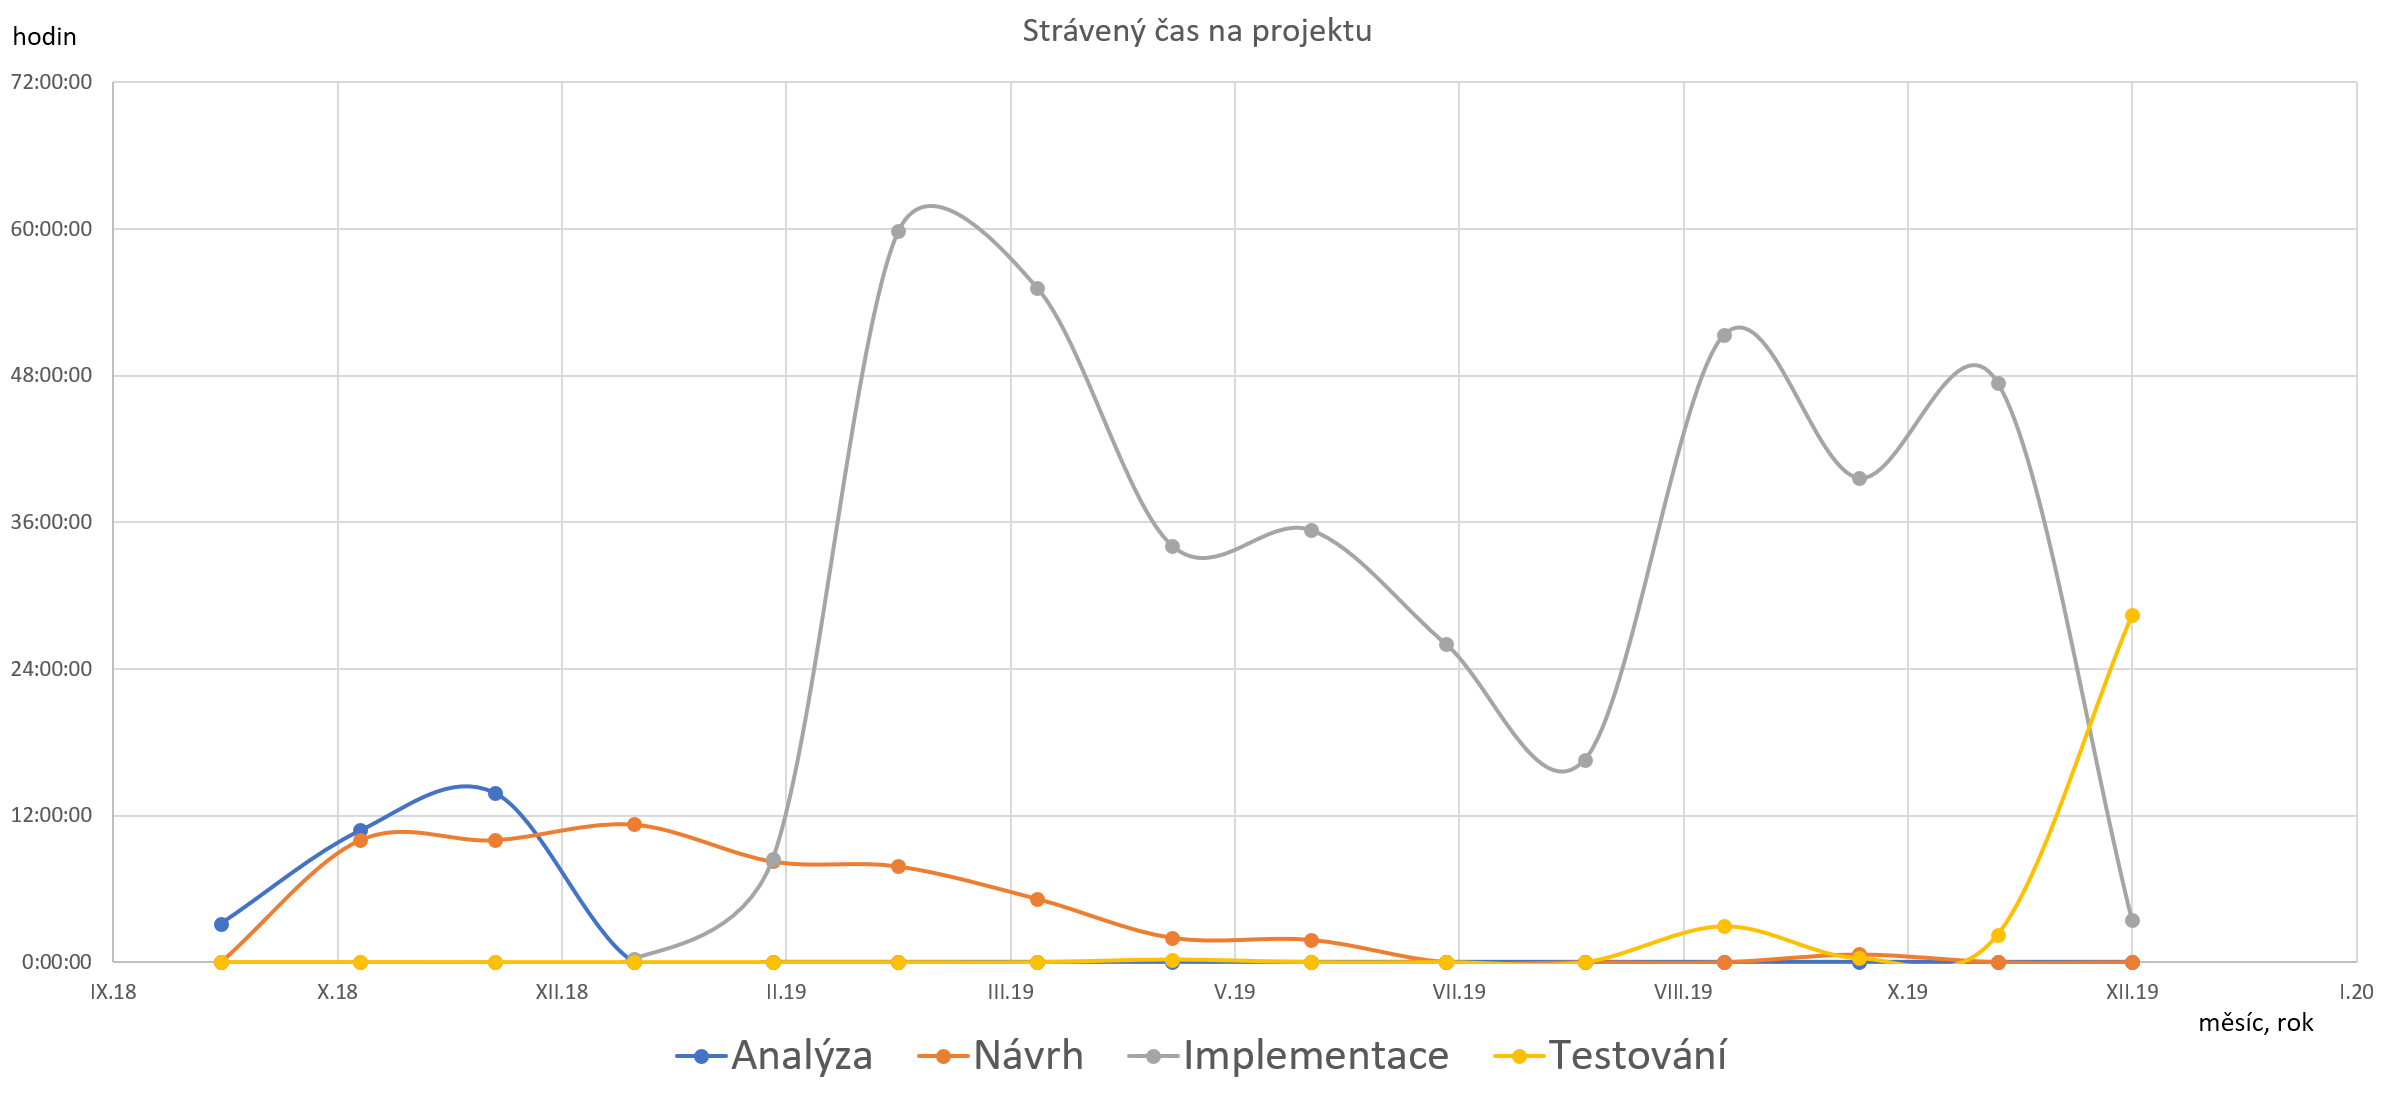
\includegraphics[width=0.9\textwidth]{../png/time/time_spent.png}
\caption[Měsíční čas strávený realizací projektu]{Čas strávený realizací projektu, rozdělený dle typu aktivity.} \label{picture:time:spent}
\end{figure}

Při zpětném ohlédnutí na tento graf vidím poměrně velkou převahu implementační části, která je způsobena tím, že analýzu jsme prováděli ještě ve dvou - společně s Pavlem Kovářem, a její efektivita byla poměrně vysoká. Naopak zejména počátky implementace, které spočívaly převážně v učení se pro mě zcela nové technologie, přinesly pochopitelnou neefektivitu samotného vývoje a tudíž nárůst stráveného času.\\
Testování eviduje rapidní nárůst až v závěru, což je způsobenou velkou časovou náročností uživatelského testování ve skladech. Přesto bylo testování realizováno i průběhu vývoje, avšak oproti závěru to bylo ve velmi malé míře.\\

\end{conclusion}


\nocite{*}
\printbibliography[title={Zdroje}]

\appendix

\chapter{Seznam použitých zkratek}
\setglossarystyle{acronyms}
\printglossary[type=\acronymtype,style=acronyms]

\chapter{Slovník pojmů}
\printglossary[type=main]

\chapter{Activity diagramy průchodu systému skladníkem} \label{ap:diagram:storekeeper}

\begin{figure}[]
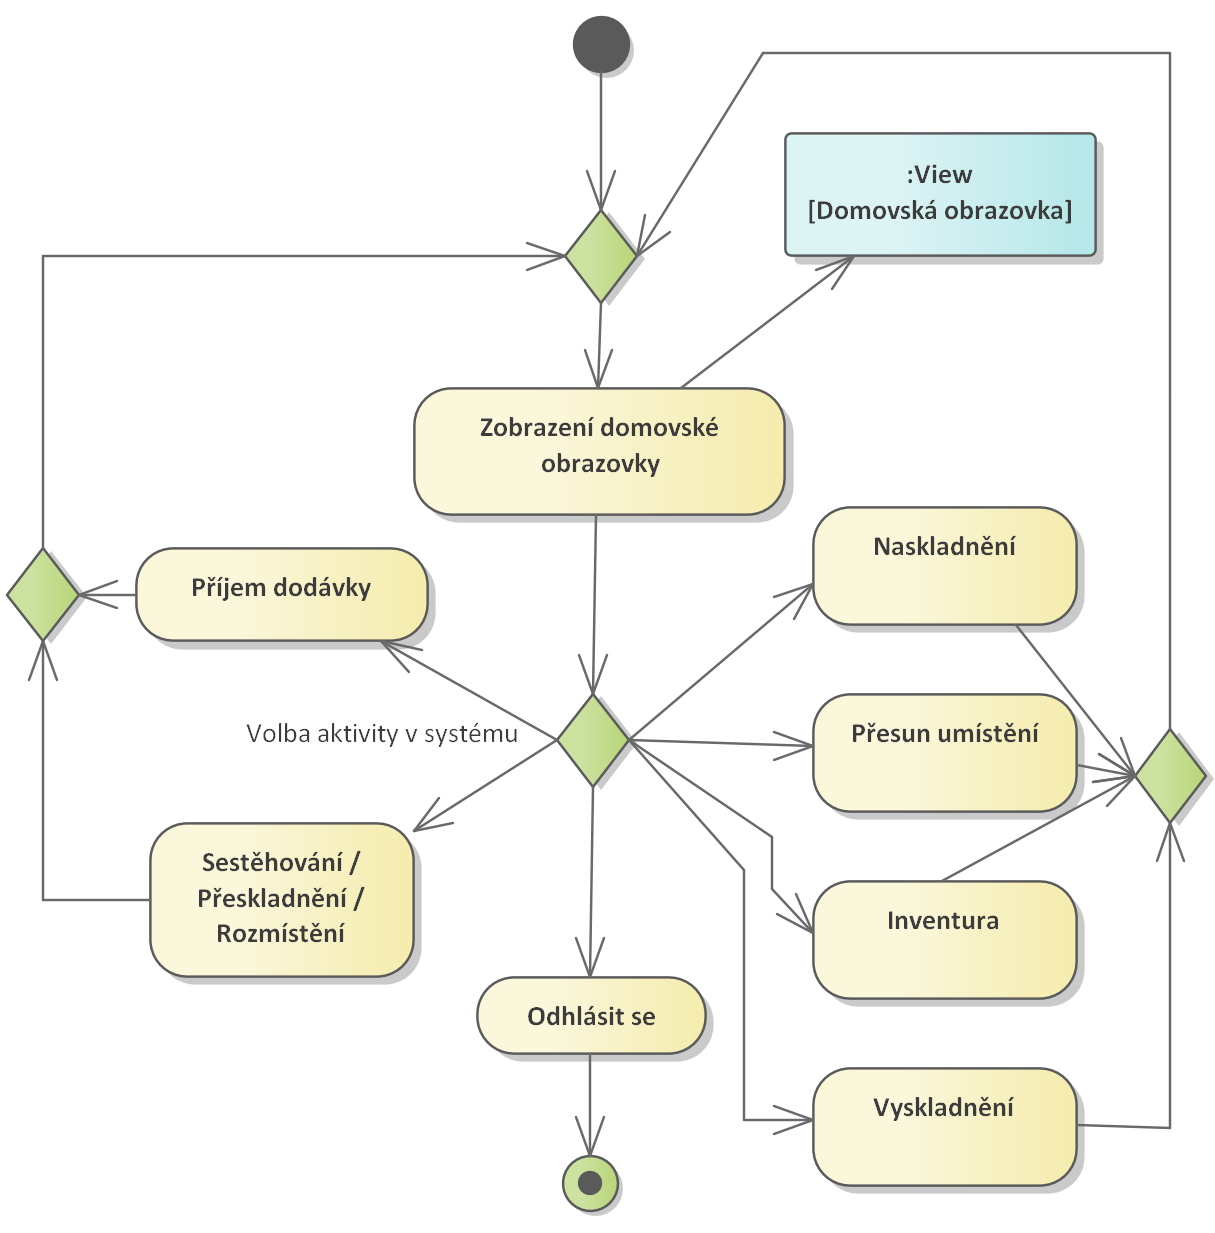
\includegraphics[width=\textwidth]{../png/diagrams/ac1.png}
\caption{Activity diagram průchodu systému skladníkem: první část} \label{picture:storekeeper1}
\end{figure}

\begin{figure}[]
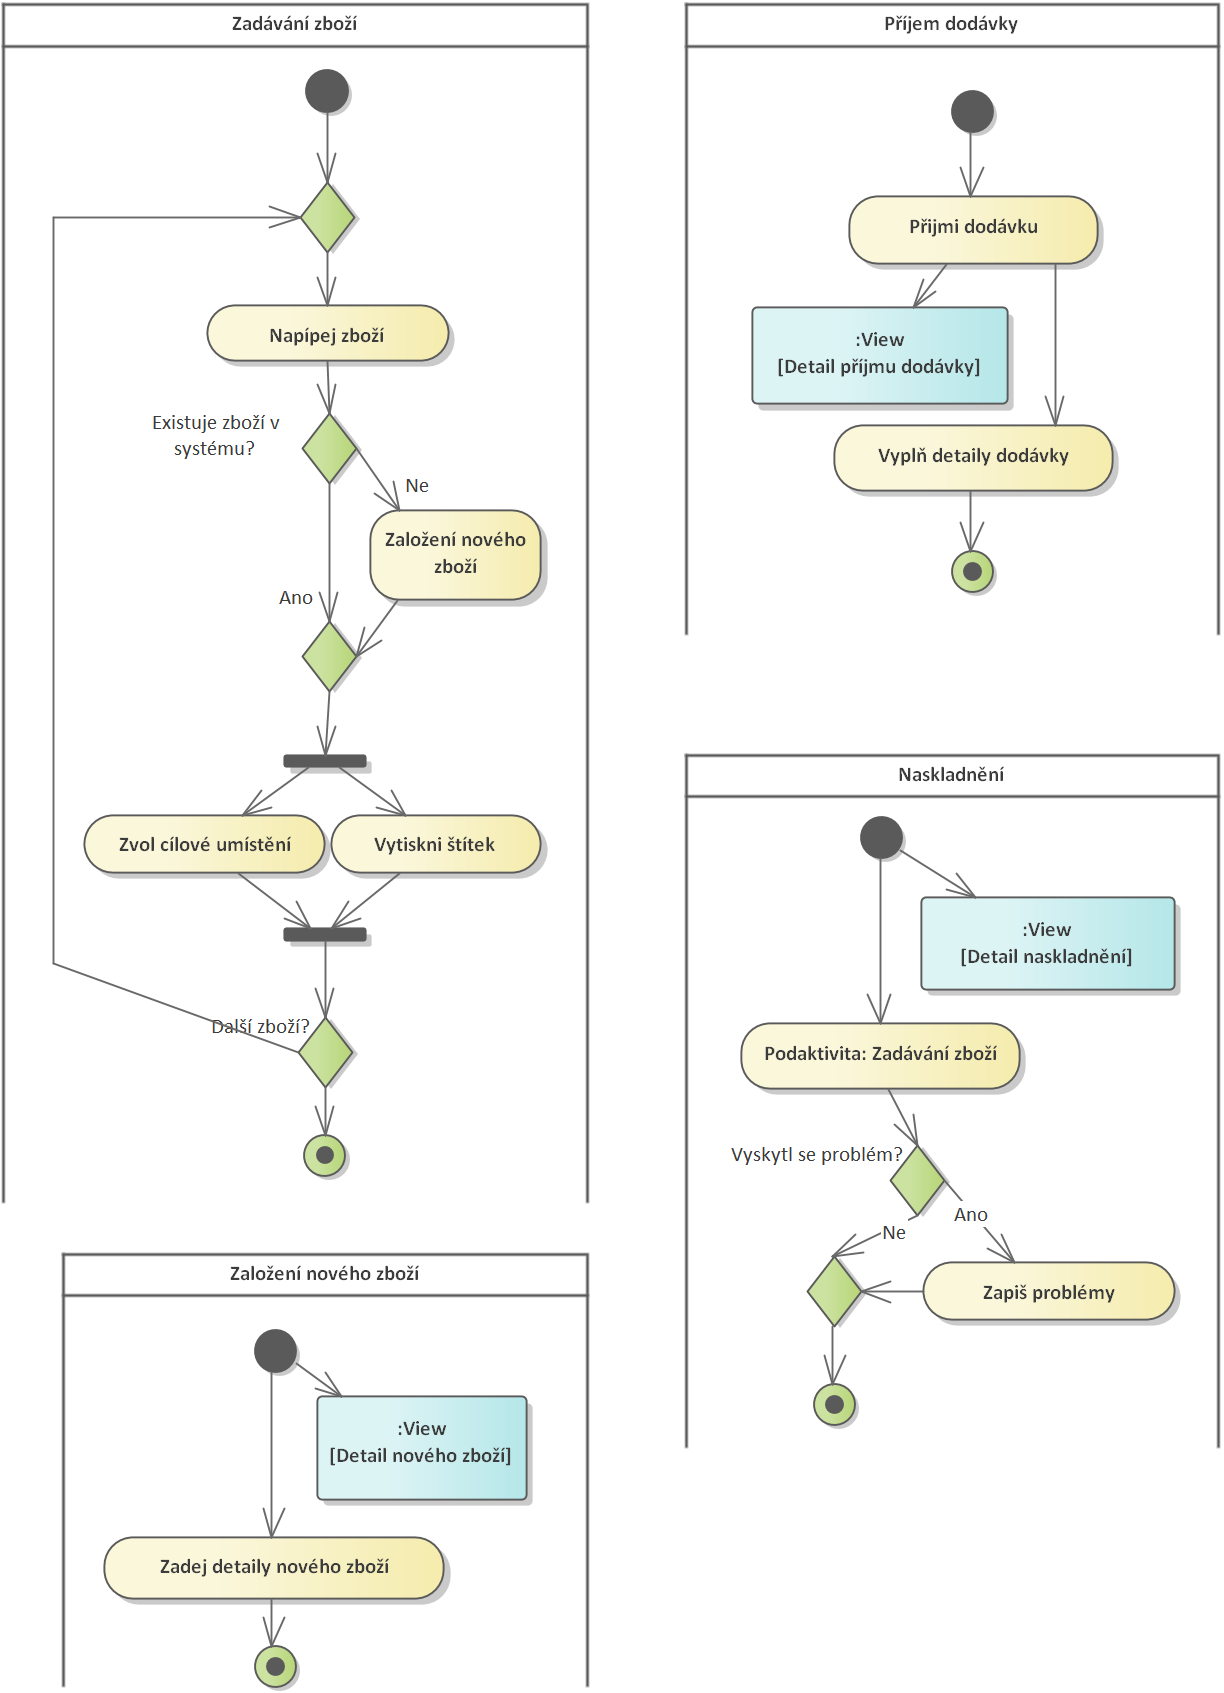
\includegraphics[width=\textwidth]{../png/diagrams/ac2.png}
\caption{Activity diagram průchodu systému skladníkem: druhá část} \label{picture:storekeeper2}
\end{figure}

\begin{figure}[]
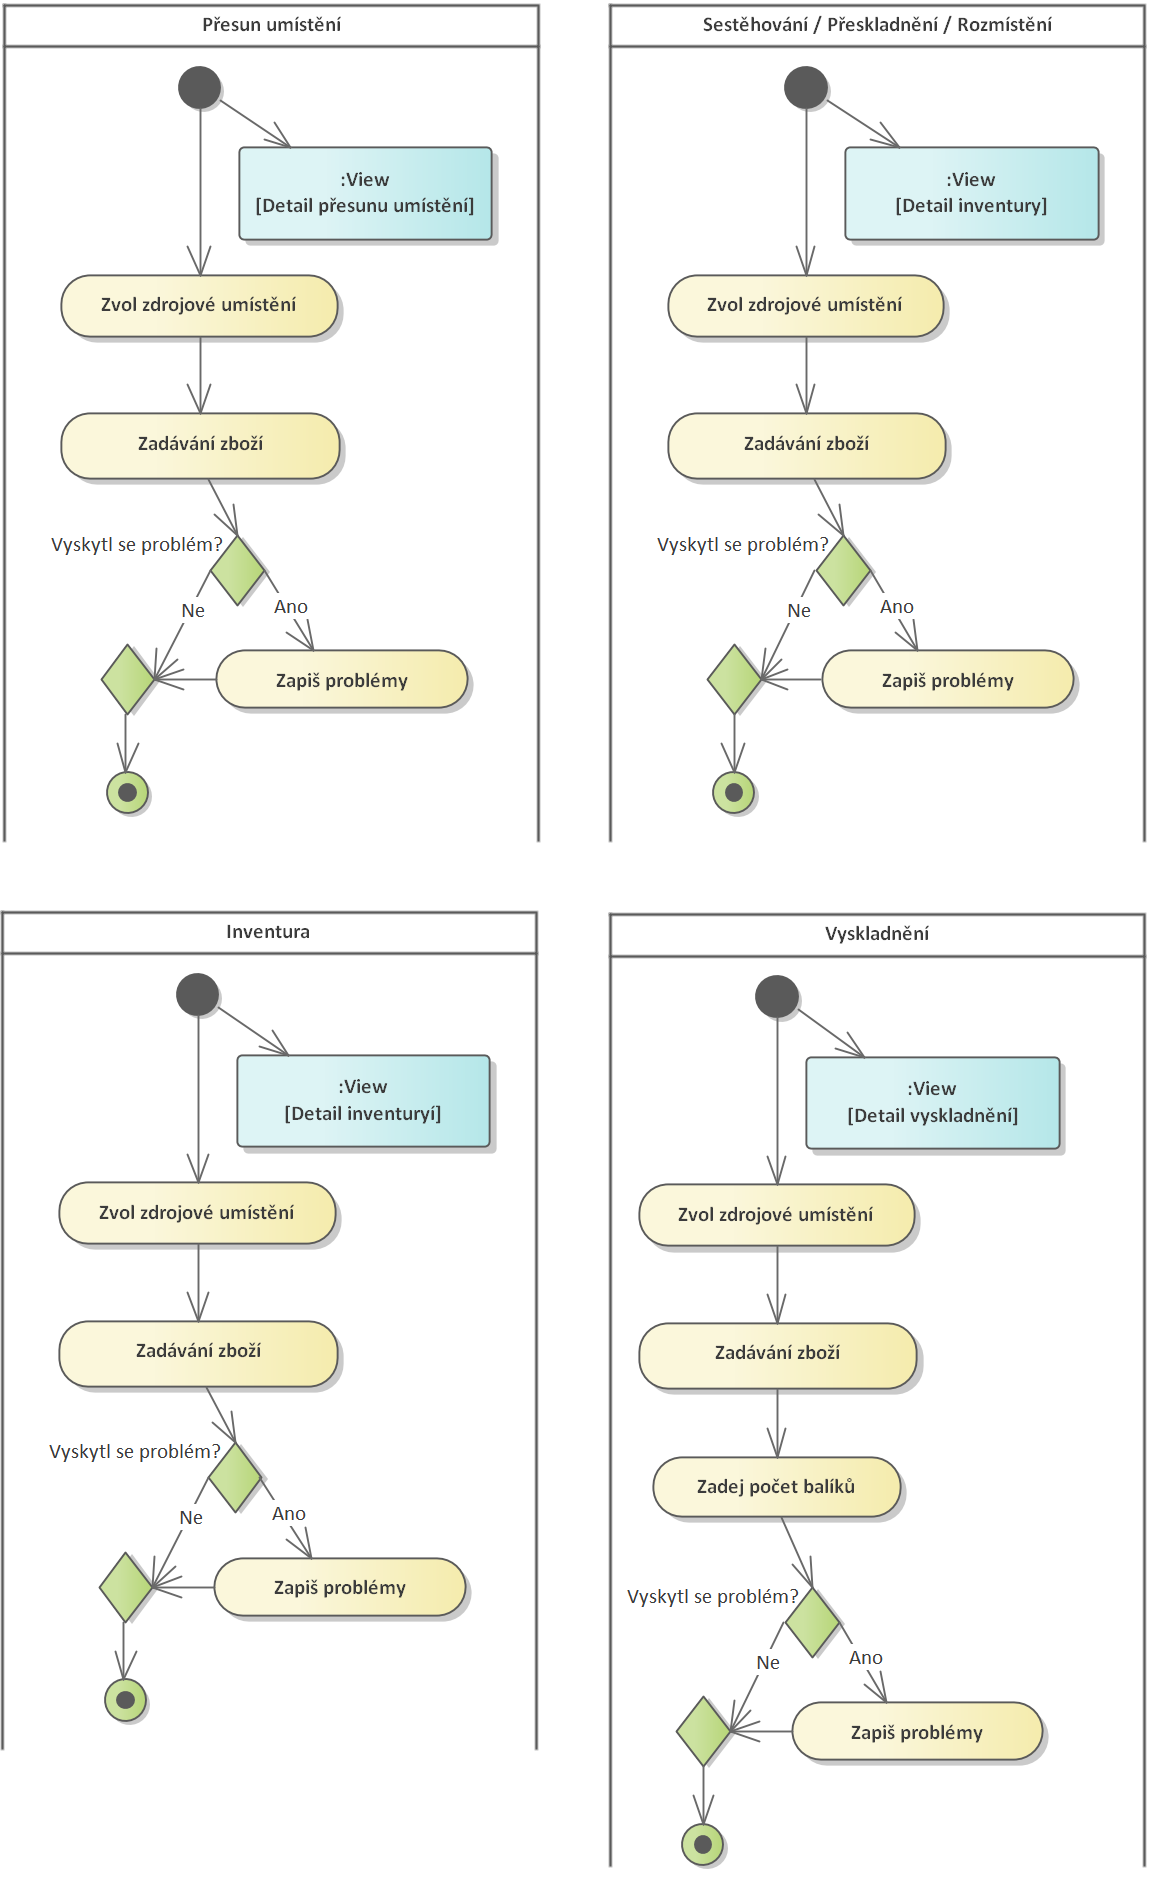
\includegraphics[height=\textheight]{../png/diagrams/ac3.png}
\caption{Activity diagram průchodu systému skladníkem: třetí část} \label{picture:storekeeper3}
\end{figure}

\chapter{Návrh procesů ve skladovém systému} \label{ap:processes}

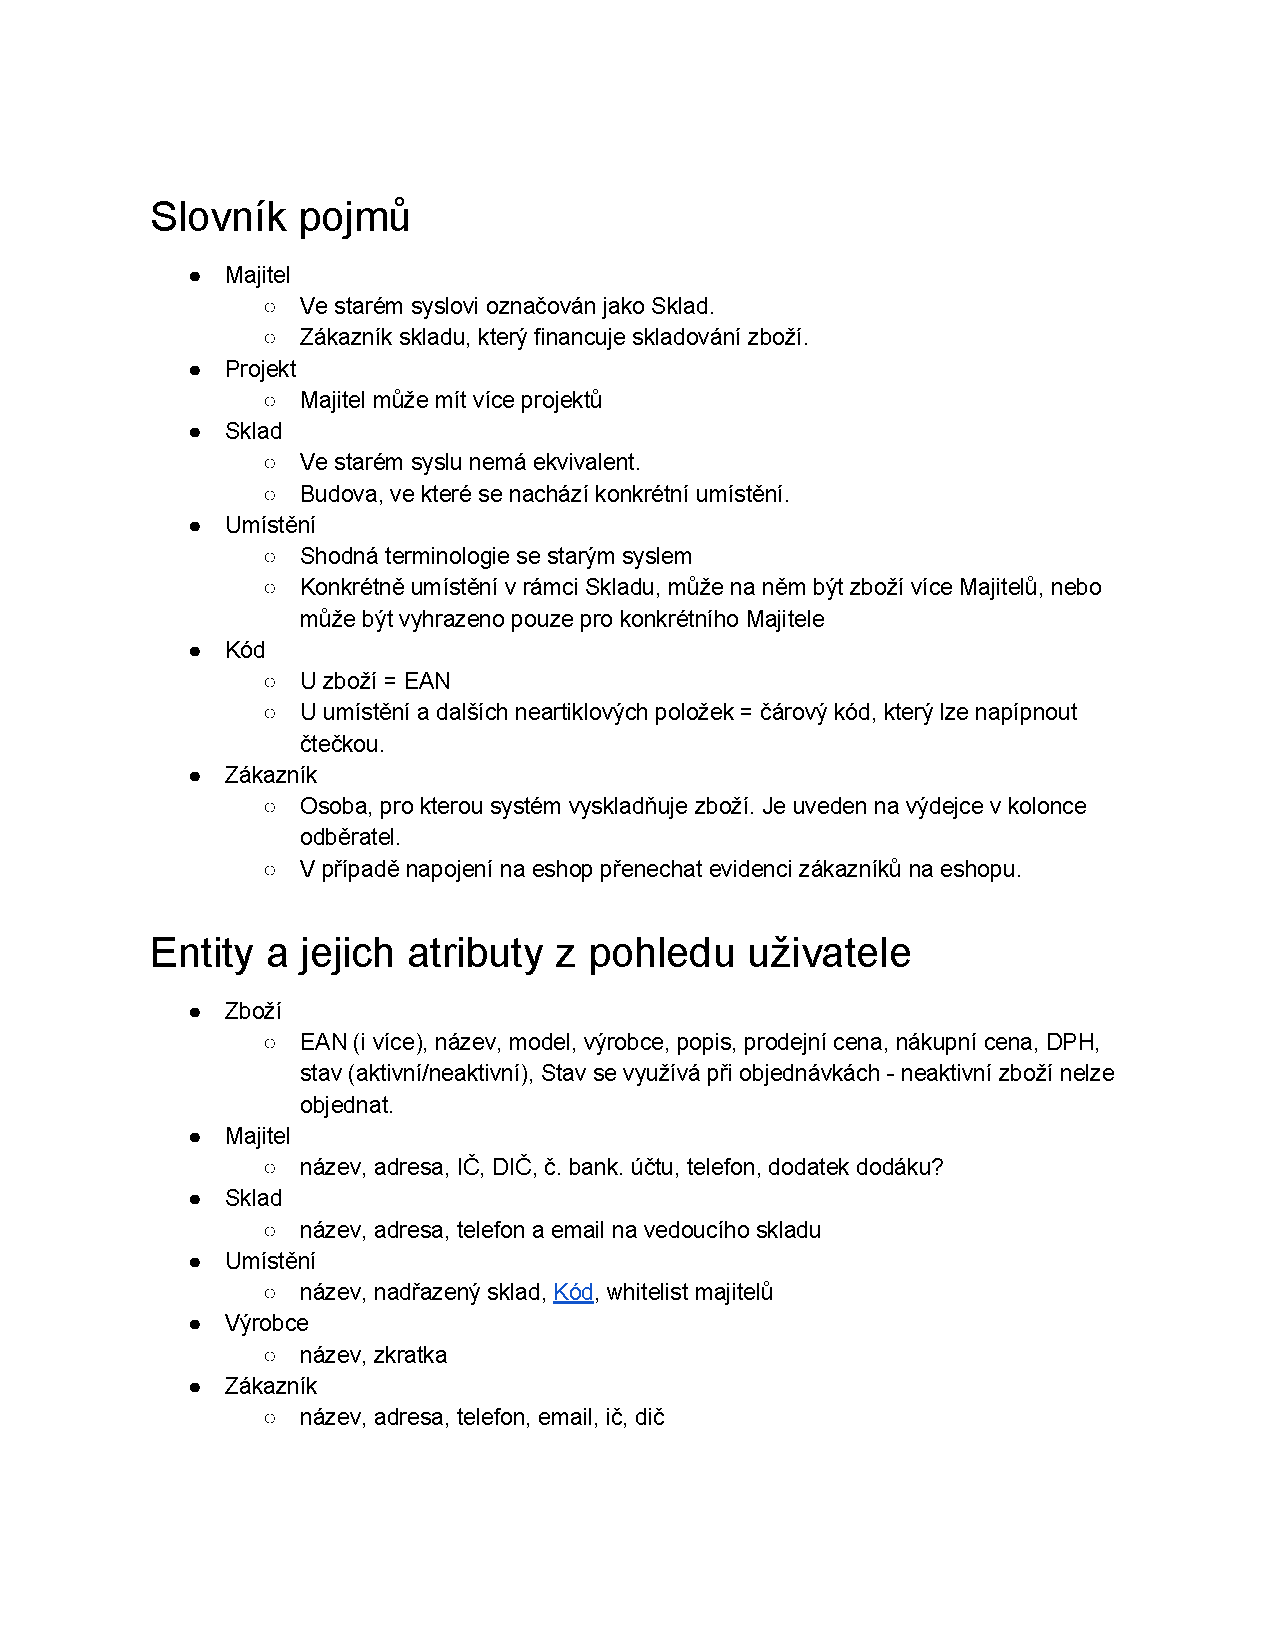
\includepdf[pages=-]{../pdf/processes.pdf}

\chapter{Zápis z uživatelského testování aplikace během vývoje} \label{ap:testing_notes}

\section{Seznam požadavků}

\begin{itemize}
	\item Na klik na šedý button formuláře ukázat, co vlastně chybí vyplnit,
	\item výchozí akce tabulky by měla být aktivní na celém řádku,
	\item karty na domovské obrazovce řadit rovnou pod sebe - jako v Google Keep,
	\item tabulky jsou moc fádní, moc splývají,
	\item přidat k úpravě skladu, co znamená volba "malý sklad",
	\item přidat ke skladu atribut "popis",
	\item v malém skladu povolit více umístění,
	\item přidat skladníkovi možnost "Rychlý přesun mezi umístěními" ,
	\item na tlačítka která pouze něco rozbalují a nepřidávají, dát jinou ikonku než "+",
	\item doplnit popisky, že umístění je fyzické a části skladu jsou virtuální,
	\item přejmenovat "první skladová položka" a "první vlastník" na reálnější údaje,
	\item přidat možnost "vytvořit nové" i přímo do tabulek, nejen v rohu obrazovky,
	\item přidat do načítání dat o subjektu nejen základní data z ARES, ale i bankovní účet, plátce DPH, nespolehlivý plátce,
	\item ve formulářích, kde se vyplňuje i IČO, ho mít na první místě, aby to uživatel vyplňoval jako první a zbytek jen načetl,
	\item k vlastníkovi skladu přidat pole "oddělení",
	\item backend by měl vypočítávat IBAN z čísla účtu,
	\item zákazník má mít možnost mít více doručovacích adres,
	\item veškeré inputy typu textarea dát jako rámeček, ne jen linku,
	\item naskladnění - skladník:
	\begin{itemize}
		\item přidat ke kusům "ks",
		\item umožnit zobrazení většího náhledu fotku,
		\item výběr počtu štítků k tisku,
		\item řešit, že je zboží s výhradou (poškozený obal atp.),
		\item skladník možnost přidávat fotky,
		\item k položkám ukládat jednotky, ty pak vypisovat v naskladnění (ks, litrů, kg, ...),
	\end{itemize}
	\item naskladnění - vedoucí (přehled hotového):
	\begin{itemize}
		\item umožnit rychlý náhled výrobku,
		\item zobrazovat fotku dodáku,
		\item hledání v přehledu naskladněných položek,
	\end{itemize}
	\item v záložkách na domovské obrazovce zobrazovat počty úkolů v jednotlivých seznamech,
	\item zvýraznit priority (možná udělat barevně i ikonky),
	\item přidat vedoucímu možnost vytvořit samotné naskladnění (bez dodávky),
	\item inventura:
	\begin{itemize}
		\item našeptávat umístění k napípání,
		\item zabalit detaily umístění, které nejsou aktivní,
		\item přidat autoscroll na napípnuté umístění,
		\item přidat fotku výrobku,
		\item položky na umístění zalamovat pod sebe,
		\item vedle názvu zobrazovat i EAN a kolikakusový EAN to je,
		\item přidat stránku přehledu inventury, která bude mít stejný obsah, jako se tiskne do PDF reportu.
	\end{itemize}
\end{itemize}

\section{Seznam chyb}

\begin{itemize}
	\item nelze změnit název atributu (PUT mění jen value),
	\item v příjmu dodávky se nevypisuje, kdo ji přijal, je tam "nikdo",
	\item nelze dokončit naskladnění,
	\item při odmítnutí řešení úkolu se špatně odesílají poznámky.
\end{itemize}

\section{Seznam otázek ke zjištění}

\begin{itemize}
	\item Mají tabákové výrobky jiný EAN pro jiné šarže? (možná mění jen kolky),
	\item zjistit, jak se dá na dodáky tisknout datová informace o položkách (QR kód s linkem na api),
	\item jak se řeší vyskladňování šaržovaných výrobků.
\end{itemize}

\section{Návrhy na pokročilé funkce}

\begin{itemize}
	\item Kategorie produktů,
	\item rozpis vytíženosti skladu: k tomu je potřeba řešit počet pozic na umístění, blokace pozic,
	\item routování trasy skladníka: nejdřív naber velké věci, pak teprve ty malé,
	\item řešit umístění u země (upozorňovat, že jsou u země výrobky, které se netočí),
	\item řešit systémově výrobky, které zabírají více palet (např. 3),
	\item hromadný aktualizátor dat z Aresu s výběrem diffu,
	\item příprava na dodávky zboží: vedoucí může zadávat skladníkům avizace dodávek = příprava následujícího úkolu naskadnění,
	\item skupiny "typů" skladníků + možnost pro vedoucího přiřazovat úkoly přímo skladníkům / skupinám skladníků,
	\item pokročilé nastavení domovské obrazovky: možnost nastavení množství informací na kartách úkolů,
	\item víceúrovňový konfigurovatelný Dashboard,
	\item nový úkol "kompletní inventura skladu": vychází z dokončené jiné inventury, nabízí k inveturizaci pouze to, co je např. jen na špatném umístění, zobrazuje, kde se chybějící zboží pohybovalo,
	\item nastavování práv skladníků:
	\begin{itemize}
		\item možnost tvořit nové položky?,
		\item možnost tvořit nová umístění?,
		\item pokud nemá právo a potřebuje to udělat, tak možnost "zavolej vedoucího".
	\end{itemize}
\end{itemize}

\chapter{Obsah přiloženého média} \label{ap:medium}

\vfill

\begin{dirfigure}
	\dirtree{%
		.1 README.md\DTcomment{stručný popis obsahu média}.
		.1 src.
			.2 thesis\DTcomment{zdrojové soubory textu práce}.
			.2 NUR-SYSEL.rpprj\DTcomment{zdrojové soubory Lo-Fi prototypu}.
			.2 mi-nur-sysel-master.zip\DTcomment{zdrojové soubory Hi-Fi prototypu}.
		.1 DIP\_Malec\_Oldrich\_2019.pdf\DTcomment{text práce ve formátu PDF}.
	}
\end{dirfigure}


\end{document}
